\documentclass[a4paper,10pt,fleqn]{ltjsarticle}

\usepackage[hiragino-pron]{luatexja-preset}

\usepackage{cite}

%括弧
\usepackage{delimseasy}

%二段組
\usepackage{multicol}
\setlength{\columnseprule}{.5pt} %中央の線

%見出しのフォント
\renewcommand{\headfont}{\sffamily\bfseries}


%数式
\usepackage{nccmath,amsmath,amssymb}
\usepackage{mathtools}
\usepackage{empheq} %数式の囲いに使う
\usepackage{physics}
\usepackage{bm}
\usepackage[bbsets]{jkmath} %\Nなどをつかえる
\usepackage{amsthm}

\usepackage{titletoc}

\AtEndPreamble{
%ハイパーリンク用
\usepackage{url}
\usepackage{hyperref}
\usepackage{xcolor}
\definecolor{BlueViolet}{RGB}{105,39,255}
\definecolor{mylightgray}{HTML}{DDDDDD}
\definecolor{mydarkgray}{HTML}{777777}
\hypersetup{
    colorlinks=true,
    citecolor=BlueViolet,
    linkcolor=blue!50!black,
    urlcolor=blue!70!black,
  }
\usepackage{bookmark}
}


%tcolorbox系
\usepackage[many]{tcolorbox}
\tcbuselibrary{breakable,skins,theorems}
\newtcolorbox{hosoibox}[1]{colframe=black,colback=white,coltitle=black,colbacktitle=white,boxrule=0.5pt,arc=0mm,enhanced,attach boxed title to top left={xshift=10mm,yshift=-3mm},boxed title style={frame hidden},title=#1}

%leftbar環境に注釈が入れられないことを解消する環境.名前は,tcolorboxの[t]とleftbarの組み合わせ
\newtcolorbox{tbleftline}{blanker,left=5mm,borderline west={1.1mm}{0pt}{mydarkgray}}
\newenvironment{tleftbar}{\begin{tbleftline}\setlength{\parindent}{1\zw}}{\end{tbleftline}}


\usepackage{framed,color}

% leftbar環境の色を変更
\makeatletter
\renewenvironment{leftbar}{%
  \def\FrameCommand{%
    {\color{mydarkgray}\vrule width 3pt}%
    \hspace{10pt}%
    \fboxsep=\FrameSep\colorbox{white}}%
  \MakeFramed{\hsize\hsize\advance\hsize-\width\FrameRestore}%
}{%
  \endMakeFramed%
}
\makeatother

%題名付き四角
\usepackage{ascmac}
\usepackage{fancybox}

%図に使うもの
\usepackage{tikz}
\usetikzlibrary{intersections,calc,arrows.meta,3d,mindmap}
\usepackage{tikz-3dplot}
\usepackage[marginparwidth=0pt,margin=25truemm]{geometry}
\usepackage{bxpapersize}
\usepackage[absolute,overlay]{textpos} %図の配置を好きにする

%画像
\usepackage{wrapfig}
%footnoteの変更
\renewcommand\thefootnote{{\dag}\arabic{footnote}}
\renewcommand{\thempfootnote}{{\dag}\arabic{mpfootnote}}
\interfootnotelinepenalty=10000

\usepackage{oubraces} %overunderbraces

%underbraceの文字数が多いときのためのadunderbrace
\usepackage{ifthen}
\newlength{\wdTempA}
\newlength{\wdTempB}
\newcommand{\adunderbrace}[2]{%
\settowidth{\wdTempA}{$#1$}%
\settowidth{\wdTempB}{${\scriptstyle #2}$}%
\ifthenelse{\wdTempA<\wdTempB}{%
\hspace*{.5\wdTempA}\hspace*{-.5\wdTempB}%
\underbrace{#1}_{#2}%
\hspace*{.5\wdTempA}\hspace*{-.5\wdTempB}%
}{%
\underbrace{#1}_{#2}%
}%
}%
%丸付き文字
\newcommand{\ctext}[1]{\raise0.2ex\hbox{\textcircled{\scriptsize{#1}}}}

%ユーザー定義
\newcommand{\dash}[1]{#1^\prime}
\newcommand{\ddash}[1]{#1^{\prime\prime}}
\newcommand{\dddash}[1]{#1^{\prime\prime\prime}}
\newcommand{\hodash}[2]{#2^{(#1)}}
\renewcommand{\labelenumi}{(\arabic{enumi})}%itemを(数字)に変更
\newcommand{\two}{I\hspace{-1.2pt}I}
\newcommand{\three}{I\hspace{-1.2pt}I\hspace{-1.2pt}I}
\renewcommand{\proofname}{\textgt{証明}}
\renewcommand{\qed}{\unskip\nobreak\quad\qedsymbol}


\renewcommand{\leq}{\leqq}
\renewcommand{\geq}{\geqq}
\renewcommand{\le}{\leqq}
\renewcommand{\ge}{\geqq}


\newcommand\kakko[1]{\noindent\textbf{《#1》}}

\DeclareMathOperator{\sgn}{sgn}
%タイトルページを定義
\usepackage[pagecolor=white,nopagecolor={none}]{pagecolor} % 背景色を変更するためのパッケージ

\newcommand{\tituloum}[5]{\begin{titlepage} 
    \begin{center} 
        \pagecolor{white} % 背景色をBlueVioletに設定
        \color{black} % テキストカラーを白に設定
        
        \vspace*{2\baselineskip}
        
        \rule{\textwidth}{1.6pt}\vspace*{-\baselineskip}\vspace*{2pt} 
        \rule{\textwidth}{0.4pt} 
        
        \vspace{0.75\baselineskip} 
        
        {\huge #1} 
        
        \vspace{0.75\baselineskip}
        
        \rule{\textwidth}{0.4pt}\vspace*{-\baselineskip}\vspace{3.2pt}
        \rule{\textwidth}{1.6pt}
        
        \vspace{2\baselineskip}
        
        #3
        
        \vspace*{3\baselineskip}
        
        
        {\huge #2}
        
        \vspace{0.5\baselineskip}
        
        \textit{#4}
        
        \vfill
        
        \vspace{0.3\baselineskip}
        
        #5
        
    \end{center}
\end{titlepage}}

% 数式のディスプレイスタイル設定
\everymath{\displaystyle}


%箇条書き
\usepackage[shortlabels]{enumitem}

%inputなどのプリアンブルを無視
\usepackage{docmute}

\everymath{\displaystyle}


%新設定2
\definecolor{burgundy}{rgb}{0.5, 0.0, 0.13}
\tcbset{mytheo/.style={fonttitle=\gtfamily\sffamily\bfseries\upshape,
enhanced,colframe=burgundy,colback=burgundy!2!white,colbacktitle=burgundy,
boxed title style={},
attach boxed title to top left={xshift=5mm,yshift*=-\tcboxedtitleheight/2},
before skip=25pt plus 2pt,
after skip=15pt plus 2pt
}}

%Theorem
\newtcbtheorem[number within=subsection]{theorem}{Theorem}%
{mytheo}{th}
\newcommand{\thref}[1]{{\bfseries\sffamily Theorem \ref{th:#1}}}
%Proposition
\newtcbtheorem[use counter from=theorem]{prop}{Proposition}%
{mytheo}{pr}
\newcommand{\prref}[1]{{\bfseries\sffamily Proposition \ref{pr:#1}}}
%Corollary
\newtcbtheorem[use counter from=theorem]{cor}{Corollary}%
{mytheo}{co}
\newcommand{\coref}[1]{{\bfseries\sffamily Corollary \ref{co:#1}}}
% Axiom
\newtcbtheorem[use counter from=theorem]{axiom}{Axiom}%
{mytheo}{ax}
\newcommand{\axref}[1]{{\bfseries\sffamily Axiom \ref{ax:#1}}}
%Definition
\newtcbtheorem[use counter from=theorem]{definition}{Definition}%
{mytheo,
colframe=blue!50!black,colback=blue!50!black!2!white,colbacktitle=blue!50!black,borderline south={2pt}{-2pt}{blue!50!black},}{de}
\newcommand{\deref}[1]{{\bfseries\sffamily Definition \ref{de:#1}}}
%Lemma
\newtcbtheorem[use counter from=theorem]{lemma}{Lemma}%
{mytheo,
colframe=green!50!black,colback=green!50!black!2!white,colbacktitle=green!50!black,borderline south={2pt}{-2pt}{green!50!black},}{le}
\newcommand{\leref}[1]{{\bfseries\sffamily Lemma \ref{le:#1}}}
%Example
\definecolor{charcoal}{rgb}{0.21, 0.27, 0.31}
\newtcbtheorem[use counter from=theorem]{example}{Example}%
{mytheo,
colframe=charcoal,colback=charcoal!2!white,colbacktitle=charcoal,borderline south={2pt}{-2pt}{charcoal},}{ex}
\newcommand{\exref}[1]{{\bfseries\sffamily Example \ref{ex:#1}}}



\usepackage{autobreak}

\usepackage{docmute}

\usepackage{fancyhdr}

\renewcommand{\headrulewidth}{0.4pt} % 線の太さ
\renewcommand{\headrule}{\color{black}\hrule width\headwidth height\headrulewidth \vskip-\headrulewidth} % 線の色

\pagestyle{fancy}
\fancyhf{} % 既存の設定をクリア
\fancyhead[C]{\textcolor{black}{齋藤正彦『線型代数入門』解答集}} % ヘッダーの中央にテキストを挿入
\fancyhead[R]{\textcolor{black}{\thepage}} % ヘッダーの右側にページ番号を挿入

\setcounter{secnumdepth}{2}

\begin{document}

% タイトルページの呼び出し
\tituloum{齋藤正彦『線型代数入門』解答集}{数学書解答集作成班}{}{}{\today}


\thispagestyle{empty}

\newpage
\pagenumbering{arabic}
\pagecolor{white}

\begin{multicols}{3}
  \tableofcontents
\end{multicols}

\newpage

\part*{はじめに}
\addcontentsline{toc}{part}{\texorpdfstring{はじめに}{はじめに}}

\section*{概要}
\addcontentsline{toc}{section}{\texorpdfstring{概要}{概要}}

この文書は,なまちゃんが運営する「数学書解答集作成班」が制作した,齋藤正彦著『線型代数入門』(東京大学出版会)の解答集である.

未完ではあるものの,編集の際の利便性を考慮して,オープンソースでの公開となった.それゆえ,数学的な誤りや誤植,改善案の提案などがあればぜひIssueに書き込んだり,Pull Requestを送っていただきたい\footnote{永遠の工事中}.


\section*{Special Thanks}
\addcontentsline{toc}{section}{\texorpdfstring{Special Thanks}{Special Thanks}}

掲載許可を得た方のみ\footnote{掲載されていないという方は「ニックネーム」を記入のもと,なまちゃんへ連絡していただきたい.}を敬称略で掲載する.
\begin{itemize}
  \item ねたんほ(解答の提供)
  \item まっちゃん(解答の提供)
  \item かねこ(解答の提供)
  \item qwer(解答の提供)
  \item やたろう(解答の提供,Git管理)
  \item 不自然対数(\LaTeX 関連)
\end{itemize}

その他,多くの方々.

\newpage
\part*{第1章}
\addcontentsline{toc}{part}{\texorpdfstring{第1章}{第1章}}

\section*{p5:問1}
\addcontentsline{toc}{section}{\texorpdfstring{p5:問1}{p5:問1}}

\begin{tleftbar}
  \begin{proof}
    線分$\mathrm{PQ}$の中点を$\mathrm{M}$とする.このとき,
    \begin{align*}
      \overrightarrow{\mathrm{OM}} & = \overrightarrow{\mathrm{OP}} + \overrightarrow{\mathrm{PM}} \\
                                   & = \bm{a} + \frac{\bm{b}-\bm{a}}{2}                            \\
                                   & = \frac{\bm{a}+\bm{b}}{2}
    \end{align*}
    である.
  \end{proof}
\end{tleftbar}
\section*{p5:問2}
\addcontentsline{toc}{section}{\texorpdfstring{p5:問2}{p5:問2}}
\begin{tleftbar}
  \begin{proof}
    三角形$\mathrm{PQR}$の重心を$\mathrm{G}$,$\mathrm{PQ}$の中点を$\mathrm{N}$とする.$\mathrm{G}$は線分$\mathrm{RN}$を$2:1$に内分する点なので,
    \begin{align*}
      \overrightarrow{\mathrm{OG}} & = \overrightarrow{\mathrm{OR}} + \frac{2}{3} \overrightarrow{\mathrm{RN}} \\
                                   & = \bm{c}+ \frac{2}{3} \left (\frac{\bm{a}+\bm{b}}{2}-\bm{c} \right)       \\
                                   & = \frac{\bm{a}+\bm{b}+\bm{c}}{3}
    \end{align*}
    である.
  \end{proof}
\end{tleftbar}

\newpage

\section*{p7:問-(上)}
\addcontentsline{toc}{section}{\texorpdfstring{p7:問-(上)}{p7:問-(上)}}


\begin{tleftbar}
  求めるベクトルを,$\bm{x}=(x,y,z)$~(ただし$x^2+y^2 +z^2=1$)とおく.
  このとき,内積の定義により,
  \begin{align*}
     & \bm{x} \cdot
    \begin{pmatrix}
      1 \\
      1 \\
      1
    \end{pmatrix}
    =x+y+z= 1 \cdot \sqrt{3} \cdot \cos \frac{\pi}{6} =\frac{3}{2} \\
     & \bm{x} \cdot
    \begin{pmatrix}
      1 \\
      1 \\
      4
    \end{pmatrix}
    =x+y+4z= 1 \cdot 3\sqrt{2} \cdot \cos \frac{\pi}{4} =3
  \end{align*}
  これらの式から,
  \begin{equation*}
    \begin{pmatrix}
      x \\
      y \\
      z
    \end{pmatrix}
    =
    \begin{pmatrix}
      (2 \pm \sqrt{2})/4 \\
      (2 \mp \sqrt{2})/4 \\
      1/2
    \end{pmatrix}
    \quad (\text{複号同順})
  \end{equation*}
  である.
\end{tleftbar}
\section*{p7:問-(下)}
\addcontentsline{toc}{section}{\texorpdfstring{p7:問-(下)}{p7:問-(下)}}
\begin{tleftbar}
  [1.4]の結果を利用する.

  求める三角形の面積を$S$とし.
  \[
    \bm{a}=\overrightarrow{\mathrm{P_1 P_2}}=(x_2-x_1,y_2-y_1,z_2-z_1),\quad \bm{b}=\overrightarrow{\mathrm{P_1 P_3}}=(x_3-x_1,y_3-y_1,z_3-z_1)
  \]
  とおく,
  このとき,
  \begin{align*}
    S & = \frac{1}{2} \sqrt{\norm{\overrightarrow{\mathrm{P_1 P_2}}}^2 \norm{\overrightarrow{\mathrm{P_1 P_3}}}^2 - (\overrightarrow{\mathrm{P_1 P_2}}, \overrightarrow{\mathrm{P_1 P_3}})^2} \\
      & = \frac{1}{2} \sqrt{\norm{\bm{a}}^2 \norm{\bm{b}}^2 - (\bm{a},\bm{b})^2 }                                                                                                             \\
      & = \frac{1}{2} \{ \lbrack (x_2 - x_1)^2+(y_2-y_1)^2+ (z_2 - z_1)^2 \rbrack \lbrack (x_3 - x_1)^2+(y_3-y_1)^2+ (z_3 - z_1)^2 \rbrack                                                    \\
      & \qquad - \lbrack (x_2-x_1)(x_3-x_1)+(y_2 -y_1)(y_3-y_1)+(z_2-z_1)(z_3-z_1)\rbrack ^2\}^{\frac{1}{2}}
  \end{align*}
  である.
\end{tleftbar}

\newpage

\section*{p8:問1}
\addcontentsline{toc}{section}{\texorpdfstring{p8:問1}{p8:問1}}


\subsection*{p8:問1-(イ)}
\addcontentsline{toc}{subsection}{\texorpdfstring{p8:問1-(イ)}{p8:問1-(イ)}}

\begin{tleftbar}
  与えられた直線を$l$とする.$l$の方程式に$x=-1$を代入すると,$y=2$となるため,$l$は点$(-1,2)$を通る.
  また,$l$は点$(2,0)$を通るため,
  $l$の方向ベクトルのひとつは,
  \[
    \begin{pmatrix}
      2-(-1) \\
      0-2
    \end{pmatrix}
    =
    \begin{pmatrix}
      3 \\
      -2
    \end{pmatrix}
  \]
  である.よって,$l$のベクトル表示のひとつは,
  $
    \begin{pmatrix}
      x \\
      y
    \end{pmatrix}
    =
    \begin{pmatrix}
      2 \\
      0
    \end{pmatrix}
    +t
    \begin{pmatrix}
      3 \\
      -2
    \end{pmatrix}
    ~(-\infty < t < \infty)$である.
\end{tleftbar}


\subsection*{p8:問1-(ロ)}
\addcontentsline{toc}{subsection}{\texorpdfstring{p8:問1-(ロ)}{p8:問1-(ロ)}}

\begin{tleftbar}
  与えられた直線を$l'$とする.$l '$の方向ベクトルのひとつは,$
    \begin{pmatrix}
      0 \\
      1
    \end{pmatrix}
  $である.また,$l '$は点$(3,0)$を通るので,そのベクトル表示のひとつは,
  $
    \begin{pmatrix}
      x \\
      y
    \end{pmatrix}
    =
    \begin{pmatrix}
      3 \\
      0
    \end{pmatrix}
    +t
    \begin{pmatrix}
      0 \\
      1
    \end{pmatrix}
    ~(-\infty < t < \infty)
  $となる.
\end{tleftbar}

\section*{p8:問2}
\addcontentsline{toc}{section}{\texorpdfstring{p8:問2}{p8:問2}}


\subsection*{p8:問2-(イ)}
\addcontentsline{toc}{subsection}{\texorpdfstring{p8:問2-(イ)}{p8:問2-(イ)}}

\begin{tleftbar}
  与えられたベクトル表示から.
  \begin{align*}
    \begin{cases}
      x=1+2t \\
      y=-1+t
    \end{cases}
  \end{align*}
  であるから,
  \begin{align*}
    \begin{cases}
      t=\frac{x-1}{2} \\
      t=y+1
    \end{cases}
  \end{align*}
  である.これから$t$を消去すると,
  \begin{gather*}
    \frac{x-1}{2} = y+1 \\
    \therefore ~ x-2y-3 =0
  \end{gather*}
  である.
\end{tleftbar}


\subsection*{p8:問2-(ロ)}
\addcontentsline{toc}{subsection}{\texorpdfstring{p8:問2-(ロ)}{p8:問2-(ロ)}}

\begin{tleftbar}
  点$(-1,-2)$を通り,$x$軸に平行な直線を表すから,$y=-2$が求める直線の方程式である.
\end{tleftbar}
%
\newpage
%
%

\section*{p10:問1}
\addcontentsline{toc}{section}{\texorpdfstring{p10:問1}{p10:問1}}

\begin{tleftbar}
  \begin{align*}
    \begin{cases}
      x+2y+3z=1 \\
      3x+2y+z=-1
    \end{cases}
  \end{align*}
  から,
  \begin{gather*}
    -2x+2z=2 \\
    \therefore \quad -x+z=1
  \end{gather*}
  である.このとき,$
    \begin{pmatrix}
      x \\
      z
    \end{pmatrix}
    =
    \begin{pmatrix}
      1 \\
      2
    \end{pmatrix}
    ,
    \begin{pmatrix}
      2 \\
      3
    \end{pmatrix}
  $はこれを満たす.このときの$y$の値を計算すると,それぞれ$-3,-5$なので,結局,与えられた直線は2点$(1,-3,2),(2,-5,3)$を通る.
  すなわち,この直線の方向ベクトルのひとつは
  \[
    \begin{pmatrix}
      2  \\
      -5 \\
      3
    \end{pmatrix}
    -
    \begin{pmatrix}
      1  \\
      -3 \\
      2
    \end{pmatrix}
    =
    \begin{pmatrix}
      1  \\
      -2 \\
      1
    \end{pmatrix}
  \]
  である.したがって求めるベクトル表示のひとつは,直線上の任意の位置ベクトルを$\bm{x}$とすると,
  \[
    \bm{x} =
    \begin{pmatrix}
      1  \\
      -3 \\
      2
    \end{pmatrix}
    +t
    \begin{pmatrix}
      1  \\
      -2 \\
      1
    \end{pmatrix}
  \]
  と表せる.
\end{tleftbar}

\section*{p10:問2}
\addcontentsline{toc}{section}{\texorpdfstring{p10:問2}{p10:問2}}

\begin{tleftbar}
  \begin{proof}
    $t$を$0 \le t \le 1$をみたす実数,線分$\mathrm{P_1 P_2}$上の任意の点の位置ベクトルを$\bm{x}$とする.
    このとき,
    \begin{align*}
      \bm{x} & = \overrightarrow{\mathrm{O P_1}}+t\overrightarrow{\mathrm{P_1 P_2}} \\
             & = \bm{x}_1 + t (\bm{x}_2 - \bm{x}_1)                                 \\
             & = (1-t) \bm{x}_1 + t \bm{x}_2
    \end{align*}
    である.$1-t = t_1,~t=t_2$と改めておくと,$t$の定め方から$t_1 \ge 0,~t_2 \ge 0$であり,
    \[
      \bm{x}= t_1 \bm{x}_1 + t_2 \bm{x}_2 ,\quad t_1 + t_2 =1
    \]
    となり,これが証明すべきことであった.
  \end{proof}
\end{tleftbar}

\newpage
\section*{p11:問1}
\addcontentsline{toc}{section}{\texorpdfstring{p11:問1}{p11:問1}}

\begin{tleftbar}
  与えられた平面を$(S)$とおく.$(S)$は3点$(-1,0,1),~(2,0,-1),~(0,-1,0)$を通るので,
  \begin{equation*}
    \bm{x}_1=
    \begin{pmatrix}
      -1 \\
      0  \\
      1
    \end{pmatrix}
    ,\quad \bm{x}_2=
    \begin{pmatrix}
      2 \\
      0 \\
      -1
    \end{pmatrix}
    \quad
    \bm{x}_3=
    \begin{pmatrix}
      0  \\
      -1 \\
      0
    \end{pmatrix}
  \end{equation*}
  と改めておくと,
  \begin{gather*}
    \bm{x}_2 - \bm{x}_1 =
    \begin{pmatrix}
      3 \\
      0 \\
      -1
    \end{pmatrix}
    ,\quad
    \bm{x}_3 - \bm{x}_1 =
    \begin{pmatrix}
      1  \\
      -1 \\
      -1
    \end{pmatrix}
  \end{gather*}
  となり,$\bm{x}_2 - \bm{x}_1$と$\bm{x}_3 - \bm{x}_1$は線型独立なので,求めるベクトル表示のひとつは,
  \[
    (S) \colon \bm{x}=
    \begin{pmatrix}
      -1 \\
      0  \\
      1
    \end{pmatrix}
    + t
    \begin{pmatrix}
      3 \\
      0 \\
      -1
    \end{pmatrix}
    +s
    \begin{pmatrix}
      1  \\
      -1 \\
      -1
    \end{pmatrix}
    ~( -\infty < t,~s<\infty)
  \]
\end{tleftbar}
%
%
%
%
\section*{p12:問2}
\addcontentsline{toc}{section}{\texorpdfstring{p12:問2}{p12:問2}}

\begin{tleftbar}
  \begin{align*}
    \begin{cases}
      x=1+t-s   \\
      y=2-t -2s \\
      z=0+2t+s
    \end{cases}
  \end{align*}
  から$t$と$s$を消去して,
  \[
    x-y-z=-1
  \]
  これが求める直線の方程式である.
\end{tleftbar}

\section*{p12:問3}
\addcontentsline{toc}{section}{\texorpdfstring{p12:問3}{p12:問3}}

\begin{tleftbar}
  \begin{proof}
    \[
      \overrightarrow{\mathrm{OP_1}}=\bm{x}_1,\quad \overrightarrow{\mathrm{OP_2}}=\bm{x}_2,\quad \overrightarrow{\mathrm{OP_3}}=\bm{x}_3
    \]
    とする.このとき,三角形$\mathrm{P_1 P_2 P_3}$上の任意の点の位置ベクトルを$\bm{x}$,$s,t$を$0 \le s,t \le 1$を満たす実数とすると,
    \begin{gather*}
      \bm{x}=\bm{x}_1 + s(\bm{x}_2 - \bm{x}_1) + t (\bm{x}_3 - \bm{x}_1) \\
      \therefore \quad \bm{x} = (1-s-t)\bm{x}_1 + s\bm{x}_2 + t \bm{x}_3
    \end{gather*}
    となり,$1-s-t=t_1,~s=t_2,~t=t_3$と改めて書き直すと,$s,t$の定め方より,$0 \le t_1 ,t_2,t_3 \le 1$であり
    \[
      \bm{x} = t_1\bm{x}_1 + t_2\bm{x}_2 + t_3 \bm{x}_3,\quad t_1+t_2+t_3=1
    \]
    となる.これが証明すべきことであった.
  \end{proof}
\end{tleftbar}
%
\newpage
%
\section*{p13:問1}
\addcontentsline{toc}{section}{\texorpdfstring{p13:問1}{p13:問1}}
%
\begin{tleftbar}
  $(S_1)$,$(S_2)$の法線ベクトルをそれぞれ$\bm{x}_1$,$\bm{x}_2$とおくと,
  \begin{gather*}
    \bm{x}_1 =
    \begin{pmatrix}
      1 \\
      1 \\
      2
    \end{pmatrix}
    ,
    \bm{x}_2 =
    \begin{pmatrix}
      3 \\
      3 \\
      0
    \end{pmatrix}
  \end{gather*}
  である.ゆえに,交角を$\theta ~(0 \le \theta \le \frac{\pi}{2})$とすると,
  \[
    \cos \theta = \frac{\bm{x}_1 \cdot \bm{x}_2}{\norm{\bm{x}_1} \norm{\bm{x}_2}}=\frac{3}{3\sqrt{2}}=\frac{1}{\sqrt{2}}
  \]
  であるから,$0 \le \theta \le \frac{\pi}{2}$より$\theta =\frac{\pi}{4}$である.
\end{tleftbar}
%
\section*{p13:問2}
\addcontentsline{toc}{section}{\texorpdfstring{p13:問2}{p13:問2}}

\begin{tleftbar}
  \begin{proof}
    平面$\pi_1$,$\pi_2$を考え,$\pi_1$,$\pi_2$の法線ベクトルをそれぞれ$\bm{n}_1$,$\bm{n}_2$とおく.
    \begin{description}
      \item[$\bm{n}_1$と$\bm{n}_2$が平行なとき] \mbox{}\\
            $\pi_1$に垂直な平面は$\pi_2$にも垂直であり,このような平面を$\pi_3$とすると,
            $\pi_3$は$\bm{n}_1$,$\bm{n}_2$と平行である.よって$\pi_3$と$\pi_1$,$\pi_2$はそれぞれ並行であり,このような平面は確かに存在する.
      \item[$\bm{n}_1$と$\bm{n}_2$が平行でないとき] \mbox{} \\
            $\bm{n}_1 , \bm{n}_2 \ne \bm{0}$は明らかなので,$\bm{n}_3 \coloneqq \bm{n}_1 \times \bm{n}_2$とすると,
            $\bm{n}_3 \ne \bm{0}$である.よって,$\bm{n}_3$は$\pi_1$,$\pi_2$に垂直である.このとき$n_3$を法線ベクトルとする平面を取ればよい.
    \end{description}
    以上の考察により証明された.
  \end{proof}
\end{tleftbar}
\newpage
%
%
%
\section*{p18:問}
\addcontentsline{toc}{section}{\texorpdfstring{p18:問}{p18:問}}

\begin{tleftbar}
  \begin{proof}
    $A$,$B$,$C$が$2 \times 2$行列の場合を証明する.
    \begin{gather*}
      A=
      \begin{pmatrix}
        a & b \\
        c & d
      \end{pmatrix}
      ,
      B=
      \begin{pmatrix}
        e & f \\
        g & h
      \end{pmatrix}
      ,C=
      \begin{pmatrix}
        i & j \\
        k & l
      \end{pmatrix}
    \end{gather*}
    とし,$A$,$B$,$C$の成分はすべて複素数であるとする.このとき,
    \begin{align*}
      (AB)C & =
      \begin{pmatrix}
        ae+bg & af+bh \\
        ce+dg & cf+dh
      \end{pmatrix}
      \begin{pmatrix}
        i & j \\
        k & l
      \end{pmatrix}
      \\
            & =
      \begin{pmatrix}
        aei +bgi +afk +bhk & aej+bgj+afl+bhl     \\
        cei +dgi+cfk +dhk  & cej +dgj + cfl +dhl
      \end{pmatrix}
    \end{align*}
    となる.他方
    \begin{align*}
      A(BC) & =
      \begin{pmatrix}
        a & b \\
        c & d
      \end{pmatrix}
      \begin{pmatrix}
        ei + fk & ej +fl \\
        gi + hk & gj +hl
      \end{pmatrix}
      \\
            & =
      \begin{pmatrix}
        aei + afk +bgi +bhk  & aej +afl +bgj +bhl   \\
        cei + cfk + dgi +dhk & cej + cfl + dgi +dhl
      \end{pmatrix}
    \end{align*}
    となり,たしかに$(AB)C=A(BC)$である.
  \end{proof}
\end{tleftbar}
%
\newpage
\section*{p19:問1-(上)}
\addcontentsline{toc}{section}{\texorpdfstring{p19:問1-(上)}{p19:問1-(上)}}
%
%
\begin{tleftbar}
  \begin{proof}
    \[
      \begin{pmatrix}
        -1 & 0  \\
        0  & -1
      \end{pmatrix}
      \begin{pmatrix}
        x \\
        y
      \end{pmatrix}
      =
      \begin{pmatrix}
        -x \\
        -y
      \end{pmatrix}
    \]
    となり,これは明らかに線型変換である.対応する行列は,$
      \begin{pmatrix}
        -1 & 0  \\
        0  & -1
      \end{pmatrix}
    $である.
  \end{proof}
\end{tleftbar}

\section*{p19:問2-(上)}
\addcontentsline{toc}{section}{\texorpdfstring{p19:問2-(上)}{p19:問2-(上)}}
\begin{tleftbar}
  \begin{proof}
    式(15)より,$2 \times 2$行列$A$,$B$とベクトル$\bm{x}$について,
    \begin{align*}
      T_B (T_A (\bm{x})) & = B(A\bm{x})      \\
                         & = (BA) \bm{x}     \\
                         & = T_{BA} (\bm{x})
    \end{align*}
    である.これが証明すべきことであった.
  \end{proof}
\end{tleftbar}


\section*{p19:問1-(下)}
\addcontentsline{toc}{section}{\texorpdfstring{p19:問1-(下)}{p19:問1-(下)}}

\begin{tleftbar}
  $\bm{x} =
    \begin{pmatrix}
      x \\
      y
    \end{pmatrix}
  $
  とおくと,(17)式より,
  \begin{align*}
    T \bm{x} & = \frac{ax+by}{a^2+b^2} \bm{a} \\
             & =
    \begin{pmatrix}
      a^2x +aby   \\
      ab x + b^2y \\
    \end{pmatrix}
    \\
             & =
    \begin{pmatrix}
      a^2 & ab  \\
      ab  & b^2
    \end{pmatrix}
    \begin{pmatrix}
      x \\
      y
    \end{pmatrix}
    \\
             & =
    \begin{pmatrix}
      a^2 & ab  \\
      ab  & b^2
    \end{pmatrix}
    \bm{x}
  \end{align*}
  であるから,
  \[
    T=\begin{pmatrix}
      a^2 & ab  \\
      ab  & b^2
    \end{pmatrix}
  \]
  となる.
\end{tleftbar}
%
\newpage

\section*{p19:問2-(下)}
\addcontentsline{toc}{section}{\texorpdfstring{p19:問2-(下)}{p19:問2-(下)}}


\subsection*{p19:問2-(下)-(イ)}
\addcontentsline{toc}{subsection}{\texorpdfstring{p19:問2-(下)-(イ)}{p19:問2-(下)-(イ)}}
\begin{leftbar}
  \begin{proof}
    $\bm{a}=
      \begin{pmatrix}
        a_1 \\
        a_2
      \end{pmatrix}
    $,
    $\bm{b}=
      \begin{pmatrix}
        b_1 \\
        b_2
      \end{pmatrix}
    $,$\bm{a} \ne \bm{0}$かつ$\bm{b} \ne \bm{0}$とする.
    このとき,
    \begin{align*}
      T \bm{x} & =\frac{(\bm{a},\bm{x})}{(\bm{a},\bm{a})} \bm{a} \\
               & = \frac{a_1 x + a_2 y}{{a_1}^2+{a_2}^2}
      \begin{pmatrix}
        a_1 \\
        a_2
      \end{pmatrix}
      \\
               & =
      \frac{1}{{a_1}^2+{a_2}^2}
      \begin{pmatrix}
        {a_1}^2 & a_1 a_2 \\
        a_1 a_2 & {a_2}^2
      \end{pmatrix}
      \begin{pmatrix}
        x \\
        y
      \end{pmatrix}
    \end{align*}
    となる.つまり,$T=\frac{1}{{a_1}^2+{a_2}^2}
      \begin{pmatrix}
        {a_1}^2 & a_1 a_2 \\
        a_1 a_2 & {a_2}^2
      \end{pmatrix}
    $である.このとき,
    \begin{align*}
      T^2 & = \frac{1}{({a_1}^2+{a_2}^2)^2}
      \begin{pmatrix}
        {a_1}^4 + {a_1}^2 {a_2}^2 & {a_1}^3 a_2 + a_1 {a_2}^3 \\
        {a_1}^3 a_2 + a_1 {a_2}^3 & {a_2}^4 + {a_1}^2 {a_2}^2
      \end{pmatrix}
      \\
          & = \frac{1}{{a_1}^2+{a_2}^2}
      \begin{pmatrix}
        {a_1}^2 & a_1 a_2 \\
        a_1 a_2 & {a_2}^2
      \end{pmatrix}
      =T
    \end{align*}
    となり,$T^2=T$である.$S^2=S$も同様にして示される.
  \end{proof}
\end{leftbar}

\subsection*{p19:問2-(下)-(ロ)}
\addcontentsline{toc}{subsection}{\texorpdfstring{p19:問2-(下)-(ロ)}{p19:問2-(下)-(ロ)}}
\begin{tleftbar}
  \begin{proof}
    $\bm{a}=
      \begin{pmatrix}
        a_1 \\
        a_2
      \end{pmatrix}
    $,$\bm{b}=
      \begin{pmatrix}
        b_1 \\
        b_2
      \end{pmatrix}
    $とする.このとき,$\bm{a}$と$\bm{b}$が直交することから,
    \begin{gather*}
      \bm{a} \cdot \bm{b}=0 \\
      \therefore ~a_1 b_1 + a_2 b_2 =0
    \end{gather*}
    である.ここで,
    \begin{align*}
      TS & = \frac{1}{({a_1}^2 +{a_2}^2)}
      \begin{pmatrix}
        {a_1}^2 & a_1 a_2 \\
        a_1 a_2 & {a_2}^2
      \end{pmatrix}
      \frac{1}{({b_1}^2 +{b_2}^2)}
      \begin{pmatrix}
        {b_1}^2 & b_1 b_2 \\
        b_1 b_2 & {b_2}^2
      \end{pmatrix}
      \\
         & =\frac{a_1 b_1 + a_2 b_2}{({a_1}^2 +{a_2}^2)({b_1}^2 +{b_2}^2)}
      \begin{pmatrix}
        a_1 b_1 & a_1 b_2 \\
        a_2 b_1 & a_2 b_2
      \end{pmatrix}
      =O                                                                   \\
         & \qquad \qquad  (\because ~ a_1 b_1 + a_2 b_2 =0)
    \end{align*}
    である.同様に$ST$を計算すると,$ST=O$であることもわかり,これで$TS=ST=O$が証明された.
  \end{proof}
\end{tleftbar}

\subsection*{p19:問2-(下)-(ハ)}
\addcontentsline{toc}{subsection}{\texorpdfstring{p19:問2-(下)-(ハ)}{p19:問2-(下)-(ハ)}}
\begin{tleftbar}
  \begin{proof}
    イ),ロ)の文字や結論を用いると,
    \begin{align*}
      T \bm{x} + S \bm{x} & =
      \frac{1}{{a_1}^2+{a_2}^2}
      \begin{pmatrix}
        {a_1}^2 & a_1 a_2 \\
        a_1 a_2 & {a_2}^2
      \end{pmatrix}
      \begin{pmatrix}
        x \\
        y
      \end{pmatrix}
      +
      \frac{1}{{b_1}^2+{b_2}^2}
      \begin{pmatrix}
        {b_1}^2 & b_1 b_2 \\
        b_1 b_2 & {b_2}^2
      \end{pmatrix}
      \begin{pmatrix}
        x \\
        y
      \end{pmatrix}
      \\
                          & = \frac{1}{({a_1}^2+{a_2}^2)({b_1}^2+{b_2}^2)}
      \begin{pmatrix}
        ({a_1}^2+{a_2}^2)({b_1}^2+{b_2}^2) & ({a_1}^2+{a_2}^2)({b_1}^2+{b_2}^2) \\
        ({a_1}^2+{a_2}^2)({b_1}^2+{b_2}^2) & ({a_1}^2+{a_2}^2)({b_1}^2+{b_2}^2)
      \end{pmatrix}
      \begin{pmatrix}
        x \\
        y
      \end{pmatrix}
      \\
                          & =\begin{pmatrix}
                               x \\
                               y
                             \end{pmatrix}
      =\bm{x}
    \end{align*}
    となる.これが証明すべきことであった.
  \end{proof}
\end{tleftbar}

\newpage

\section*{p22:問1}
\addcontentsline{toc}{section}{\texorpdfstring{p22:問1}{p22:問1}}


\subsection*{p22:問1-(イ)}
\addcontentsline{toc}{subsection}{\texorpdfstring{p22:問1-(イ)}{p22:問1-(イ)}}
\begin{tleftbar}
  \[
    \begin{pmatrix}
      -1 & 0 & 0  \\
      0  & 1 & 0  \\
      0  & 0 & -1
    \end{pmatrix}
    \begin{pmatrix}
      x \\
      y \\
      z
    \end{pmatrix}
    =\begin{pmatrix}
      -x \\
      y  \\
      -z
    \end{pmatrix}
  \]
  となり,これは$y$軸に関する対象点に移す変換を表す.
\end{tleftbar}

\subsection*{p22:問1-(ロ)}
\addcontentsline{toc}{subsection}{\texorpdfstring{p22:問1-(ロ)}{p22:問1-(ロ)}}
\begin{tleftbar}
  \[
    \begin{pmatrix}
      1 & 0           & 0            \\
      0 & \cos \alpha & -\sin \alpha \\
      0 & \sin \alpha & \cos \alpha
    \end{pmatrix}
    \begin{pmatrix}
      x \\
      y \\
      z
    \end{pmatrix}
    =
    \begin{pmatrix}
      x                            \\
      y \cos \alpha -z \sin \alpha \\
      y \sin \alpha + z \cos \alpha
    \end{pmatrix}
  \]
  となり,これは$x$軸まわりに角$\alpha$だけ回転する変換を表す.
\end{tleftbar}

\subsection*{p22:問1-(ハ)}
\addcontentsline{toc}{subsection}{\texorpdfstring{p22:問1-(ハ)}{p22:問1-(ハ)}}

\begin{tleftbar}
  \[
    \begin{pmatrix}
      0 & 1 & 0 \\
      0 & 0 & 1 \\
      1 & 0 & 0
    \end{pmatrix}
    \begin{pmatrix}
      x \\
      y \\
      z
    \end{pmatrix}
    =\begin{pmatrix}
      y \\
      z \\
      x
    \end{pmatrix}
  \]
\end{tleftbar}


\setcounter{equation}{0}

\part*{第1章・章末問題}
\addcontentsline{toc}{part}{\texorpdfstring{第1章・章末問題}{第1章・章末問題}}


\section*{p29--30:1}
\addcontentsline{toc}{section}{\texorpdfstring{p29--30:1}{p29--30:1}}

\begin{leftbar}
  \begin{proof}
    四面体$\mathrm{P_1 P_2 P_3 P_4}$を考える.三角形$\mathrm{P_2 P_3 P_4}$の任意の周および内部の点を$\mathrm{T}$とする.
    $0 \leqq k \leqq 1$,$0 \leqq s \leqq 1$をみたす$k,s \in \mathbb{R}$によって
    \begin{align*}
      \overrightarrow{\mathrm{P_2 T}} & = k \{ s \overrightarrow{\mathrm{P_2 P_3}} + (1-s) \overrightarrow{\mathrm{P_2 P_4}} \} \\
                                      & = ks(\bm{x}_3 -\bm{x}_2) + k(1-s) (\bm{x}_4-\bm{x}_2)                                   \\
                                      & = -k\bm{x}_2 + ks \bm{x}_3 + k(1-s) \bm{x}_4
    \end{align*}
    と表される.

    さて,線分$\mathrm{P_1 T}$上の任意の点を$\mathrm{Q}$とすると,$0 \leqq t \leqq 1$をみたす$t \in \mathbb{R}$によって

    \begin{align*}
      \overrightarrow{\mathrm{P_1 Q}} & =t \overrightarrow{\mathrm{P_1 T}}                                      \\
                                      & = t\overrightarrow{\mathrm{P_2 T}} - t\overrightarrow{\mathrm{P_2 P_1}} \\
                                      & = t (-k\bm{x}_2 + ks \bm{x}_3 + k(1-s) \bm{x}_4)-t(\bm{x}_1 -\bm{x}_2)  \\
                                      & = -t\bm{x}_1 +(t-kt) \bm{x}_2 + kst \bm{x}_3 +kt(1-s) \bm{x}_4
    \end{align*}
    と表されるから,$k=4$のときの求める位置ベクトルは.
    \begin{align*}
      \bm{x} & = \bm{x}_1 + \overrightarrow{\mathrm{P_1 Q}}                     \\
             & = (1-t) \bm{x}_1 +(t-kt)\bm{x}_2 +kst \bm{x}_3 +kt(1-s) \bm{x}_4
    \end{align*}
    となり,
    \[
      (1-t)+ (t-kt)+kst + kt(1-s)=1
    \]
    であるから,$1-t = t_1$,$t-kt =t_2$,$kst = t_3$,$kt(1-s)=t_4$とおくと,
    \[
      \bm{x}= t_1 \bm{x}_1 + t_2 \bm{x}_2 + t_3 \bm{x}_3 + t_4 \bm{x}_4 , \quad t_1, t_2 ,t_3 , t_4 \geqq 0 ,\quad  t_1 +t_2 + t_3 + t_4 =1
    \]
    となり,ここまでで$k=4$の場合が示された.

    ここで,$n \geqq 4$として$k=n$のときに主張が成り立つと仮定する.
    このとき,
    \[
      t_1 \bm{x}_1 + t_2 \bm{x}_2+\dots+ t_n \bm{x}_n
    \]
    は仮定により多面体$\{ \mathrm{P}_n \}$の内部の点であり,これを簡単のために$\bm{X}_n$とおく.

    さて,$\{ \mathrm{P}_n \}$の点と$\mathrm{P}_{n+1}$とを結ぶ線分上の点は,$ 0 \leqq l \leqq 1$をみたす$l \in \mathbb{R}$によって,
    \[
      l \overbrace{(  t_1 \bm{x}_1 + t_2 \bm{x}_2+\dots+ t_n \bm{x}_n)}^{\bm{X}_n}+(1-l) \bm{x}_{n+1} , \quad t_1+t_2+\dots + t_n =1
    \]
    とかける.ここで,
    \[
      l(t_1+t_2+\dots+t_n)+(1-l)=1
    \]
    なので,$\{ \mathrm{P}_n \}$の点と$\mathrm{P}_{n+1}$とを結ぶ線分上の点はこのように表せる.

    逆に,
    \[
      \bm{x} = t_1 \bm{x}_1 + t_2 \bm{x}_2 + \dots + t_n \bm{x}_n + t_{n+1} \bm{x}_{n+1} , \quad t_1, t_2 ,\dots , t_n,t_{n+1} \geqq 0 ,\quad  t_1 +t_2 + \dots+t_n + t_{n+1} =1
    \]
    としたとき,
    \begin{align*}
      \bm{x} & =\frac{t_1 \bm{x}_1 + t_2 \bm{x}_2+\dots+ t_n \bm{x}_n}{t_1+t_2+\dots+t_n} \cdot (t_1+t_2+\dots+t_n) +t_{n+1} \bm{x}_{n+1} \\
             & = T_n \bm{X}_n + t_{n+1} \bm{x}_{n+1}
    \end{align*}
    と変形できる.ただし$T_n = t_1 + t_2 +\dots+t_n$とおいた.

    さて
    \[
      \frac{\bm{X}_n }{T_n} = \frac{t_1 \bm{x}_1 }{T_n}+ \frac{t_2 \bm{x}_2 }{T_n}+\dots +  \frac{t_n \bm{x}_n }{T_n}  \\
    \]
    であることと
    \begin{align*}
      \frac{t_1}{T_n}+\frac{t_2 }{T_n} +\dots +\frac{t_n }{T_n} & = \frac{T_n}{T_n} \\
                                                                & = 1
    \end{align*}
    であることにより,
    \[
      \frac{\bm{X}_n}{T_n}
    \]
    は,多面体$\{ \mathrm{P}_n \}$の内部の点であり.
    \[
      T_n \cdot \frac{\bm{X}_n}{T_n} + t_{n+1} \bm{x}_{n+1}
    \]
    は多面体$\{ \mathrm{P}_n \}$の内部の点と$\mathrm{P}_{n+1}$を結ぶ線分上の点である.

    よって,$k=n$のときも問題の主張が成り立つ.

    以上の考察により証明された.
  \end{proof}
\end{leftbar}

\section*{p29--30:2}
\addcontentsline{toc}{section}{\texorpdfstring{p29--30:2}{p29--30:2}}

\begin{tleftbar}
  \begin{proof}
    2点$\mathrm{P}_1$,$\mathrm{P_2}$を通る直線の方程式を$ax+by+c=0$(ただし$(a,b)=0$)とおく.
    このとき,
    \[
      \begin{cases}
        ax+by+c =0       \\
        ax_1 + by_1 +c=0 \\
        ax_2 + by_2 +c =0
      \end{cases}
    \]
    が成立する.すなわちこれは
    \[
      \begin{pmatrix}
        x   & y   & 1 \\
        x_1 & y_1 & 1 \\
        x_2 & y_2 & 1
      \end{pmatrix}
      \begin{pmatrix}
        a \\
        b \\
        c
      \end{pmatrix}
      = \bm{0}
    \]
    をみたす.これを$a$,$b$,$c$についての連立方程式とみたとき,与条件により自明でない解があり,
    \[
      \begin{vmatrix}
        x   & y   & 1 \\
        x_1 & y_1 & 1 \\
        x_2 & y_2 & 1
      \end{vmatrix}
      =0
    \]
    が成立する.転置行列の行列式はもとの行列の行列式に等しいので,行列式の交代性なども用いて,
    \[
      \begin{vmatrix}
        1 & 1   & 1   \\
        x & x_1 & x_2 \\
        y & y_1 & y_2
      \end{vmatrix}
      =0
    \]
    を得る.これが証明すべきことであった.
  \end{proof}
\end{tleftbar}



\section*{p29--30:3}
\addcontentsline{toc}{section}{\texorpdfstring{p29--30:3}{p29--30:3}}

\begin{tleftbar}
  点を以下の順で移動させる変換を考える.
  \begin{enumerate}
    \item 原点中心に$-\theta$回転させる.
    \item $x$軸に関して対称移動させる.
    \item 原点中心に$\theta$回転させる.
  \end{enumerate}
  ここで,(1)から(3)までの変換を表す行列をそれぞれ$R_{-\theta}$,$A_{x}$,$R_{\theta}$とすると.
  \begin{align*}
     & R_{-\theta} = \begin{pmatrix} \cos \theta & \sin \theta \\ -\sin \theta & \cos \theta \end{pmatrix} , \\
     & A_{x} = \begin{pmatrix} 1 & 0 \\ 0 & -1 \end{pmatrix} ,                                               \\
     & R_{\theta} = \begin{pmatrix} \cos \theta & -\sin \theta \\ \sin \theta & \cos \theta \end{pmatrix} .
  \end{align*}
  となる.よって,この変換を表す行列は
  \begin{align*}
    R_{\theta} A_x R_{-\theta} & =\begin{pmatrix} \cos \theta & -\sin \theta \\ \sin \theta & \cos \theta \end{pmatrix}
    \begin{pmatrix} 1 & 0 \\ 0 & -1 \end{pmatrix}
    \begin{pmatrix} \cos \theta & \sin \theta \\ -\sin \theta & \cos \theta \end{pmatrix}                                                                                                \\
                               & = \begin{pmatrix} \cos ^2 \theta - \sin ^2 \theta & 2\sin \theta \cos \theta \\ 2\sin \theta \cos \theta & \sin ^2 \theta -\cos ^2 \theta \end{pmatrix} \\
                               & = \begin{pmatrix} \cos 2 \theta & \sin 2 \theta \\ \sin 2\theta & -\cos 2 \theta \end{pmatrix}
  \end{align*}
  である.
\end{tleftbar}


\section*{p29--30:4}
\addcontentsline{toc}{section}{\texorpdfstring{p29--30:4}{p29--30:4}}

\begin{tleftbar}
  \begin{proof}
    以下では,直線$y= \tan \theta$に関する折り返しを$T_{\theta}$とかくことにする.

    さて,直線$ y = \tan (\theta /4) x$に関する折り返しは,
    \[
      T_{\theta/4} = \begin{pmatrix} \cos (\theta /2) & \sin (\theta /2) \\  \sin (\theta /2) & -\cos (\theta /2) \end{pmatrix}
    \]
    で表される.

    また,直線$y = \tan (-\theta /4)x$に関する折り返しは.
    \[
      T_{-\theta/4} = \begin{pmatrix} \cos (\theta /2) & -\sin (\theta/2) \\ -\sin (\theta/2) & -\cos (\theta /2) \end{pmatrix}
    \]
    で表される.

    ここで,
    \begin{align*}
      T_{\theta/4} T_{-\theta/4} & = \begin{pmatrix} \cos (\theta /2) & \sin (\theta /2) \\  \sin (\theta /2) & -\cos (\theta /2) \end{pmatrix} \begin{pmatrix} \cos (\theta /2) & -\sin (\theta/2) \\ -\sin (\theta/2) & -\cos (\theta /2) \end{pmatrix} \\
                                 & =\begin{pmatrix} \cos ^2 (\theta /2)-\sin ^2 (\theta/2) & -2\sin (\theta/2) \cos (\theta/2) \\ 2\sin (\theta/2) \cos (\theta/2) & \cos ^2 (\theta/2)-\sin ^2 (\theta/2) \end{pmatrix}                                  \\
                                 & = \begin{pmatrix} \cos \theta & -\sin \theta \\ \sin \theta & \cos \theta \end{pmatrix}
    \end{align*}
    となり,これは原点のまわりに$\theta$回転する行列を表す.

    以上の考察により証明された.
  \end{proof}
\end{tleftbar}

\section*{p29--30:5}
\addcontentsline{toc}{section}{\texorpdfstring{p29--30:5}{p29--30:5}}

\begin{tleftbar}
  任意の点$\mathrm{P}(\bm{p}),~\bm{p} \in \mathbb{R}^3$を平面$(\bm{a},\bm{x})$に対して折り返すことを考える.

  点$\mathrm{P}$から$(\bm{a},\bm{x})$におろした垂線の足は,$t \in \mathbb{R}$を用いて
  \[
    \bm{p} + t \frac{\bm{a}}{(\bm{a},\bm{a})}
  \]
  と表せ,これが平面$(\bm{a},\bm{x})$上にあるので,
  \begin{align*}
                 & (\bm{a},p+t\frac{\bm{a}}{(\bm{a},\bm{a})})=0 \\
    \therefore ~ & t=- (\bm{a},\bm{p})
  \end{align*}
  である.

  また,求める点を$\mathrm{P}' (\bm{p}')$とすると,
  \begin{align*}
    \bm{p}' & = \bm{p}+t \frac{2\bm{a}}{(\bm{a},\bm{a})}               \\
            & = \bm{p}-\frac{2(\bm{a},\bm{p})}{(\bm{a},\bm{a})} \bm{a}
  \end{align*}
  であるから,これはたしかに$V^3$の線型変換を引き起こし,その変換公式は
  \[
    \bm{x} \mapsto \bm{x}-\frac{2(\bm{a},\bm{x})}{(\bm{a},\bm{a})} \bm{a}
  \]
  である,
\end{tleftbar}

\newpage

\section*{p29--30:6}
\addcontentsline{toc}{section}{\texorpdfstring{p29--30:6}{p29--30:6}}

\subsection*{p29--30:6-(イ)}
\addcontentsline{toc}{subsection}{\texorpdfstring{p29--30:6-(イ)}{p29--30:6-(イ)}}

\begin{tleftbar}
  $(S)$と$x$軸,$y$軸,$z$軸の交点をそれぞれ$\mathrm{A}$, $\mathrm{B}$,$\mathrm{C}$とする.
  このとき,$\mathrm{A}$,$\mathrm{B}$,$\mathrm{C}$の座標は図のようになり,
  この三角錐の体積を$V$とすると,
  \begin{align*}
    V= & \frac{1}{2} \cdot \frac{1}{3} \cdot\abs{ \det (\overrightarrow{\mathrm{OA}}, \overrightarrow{\mathrm{OB}}, \overrightarrow{\mathrm{OC}})} \\
    =  & \frac{1}{6} \cdot \frac{\abs{d}^3}{\abs{abc}}= \frac{\abs{d}^3}{6\abs{abc}}
  \end{align*}
  である.ここで,$\abs{\det (\overrightarrow{\mathrm{OA}}, \overrightarrow{\mathrm{OB}}, \overrightarrow{\mathrm{OC}})}$が$\overrightarrow{\mathrm{OA}}$,$\overrightarrow{\mathrm{OB}}$,$\overrightarrow{\mathrm{OC}}$の張る平行六面体の体積を表すことを用いた.

\end{tleftbar}
%回転角
\tdplotsetmaincoords{70}{135}
\begin{tikzpicture}[tdplot_main_coords]
  %軸
  \draw[->,>=stealth,semithick](0,0,0)--(5,0,0)node[below]{$x$};%x軸
  \draw[->,>=stealth,semithick](0,0,0)--(0,5,0)node[right]{$y$};%y軸
  \draw[->,>=stealth,semithick](0,0,0)--(0,0,5)node[right]{$z$};%y軸
  \draw(0,0)node[below]{O};%原点

  \draw[dashed,semithick](3,0,0)--(0,4,0)--(0,0,7/2)--cycle;
  \fill[color=gray ,opacity=0.1] (3,0,0)--(0,4,0)--(0,0,7/2)--cycle;

  \node at (3,0,0) [above left]{$\mathrm{A} (d/a,0,0)$};
  \node at (0,4,0) [above right]{$\mathrm{B}(0,d/b,0)$};
  \node at (0,0,7/2) [right]{$\mathrm{C}(0,0,d/c)$};
\end{tikzpicture}

\subsection*{p29--30:6-(ロ)}
\addcontentsline{toc}{subsection}{\texorpdfstring{p29--30:6-(ロ)}{p29--30:6-(ロ)}}

\begin{tleftbar}
  三角形$\mathrm{ABC}$の体積を$T$,$\mathrm{O}$から平面$ABC$におろした垂線の足を$H$とすると,
  \[
    V = \frac{1}{3} \norm{\overrightarrow{\mathrm{OH}}} \cdot T
  \]
  である.ここで,
  \[
    \norm{\overrightarrow{\mathrm{OH}}}=\frac{\abs{a \cdot 0 + b \cdot 0 + c \cdot 0-d}}{\sqrt{a^2+b^2+c^2}}=\frac{\abs{d}}{\sqrt{a^2+b^2+c^2}}
  \]
  なので,イ)の結果から$V =\frac{\abs{d}^3}{6\abs{abc}}$なのを加味すると,
  \[
    T = \frac{d^2\sqrt{a^2+b^2+c^2}}{2\abs{abc}}
  \]
  である.
\end{tleftbar}

\newpage

\section*{p29--30:7}
\addcontentsline{toc}{section}{\texorpdfstring{p29--30:7}{p29--30:7}}

\subsection*{p29--30:7-(イ)}
\addcontentsline{toc}{subsection}{\texorpdfstring{p29--30:7-(イ)}{p29--30:7-(イ)}}

\begin{tleftbar}
  $\bm{a}$,$\bm{b}$,$\bm{c}$が張る平行六面体の体積は,
  \[
    \abs{\det (\bm{a},\bm{b},\bm{c})}
  \]
  で与えられる.

  一方,この平行六面体の$\mathrm{O}$,$\mathrm{B}$,$\mathrm{C}$を含む面の面積は,

  \[
    \norm{\bm{b} \times \bm{c}}
  \]

  で与えられる.

  以上の考察により,求める長さは,
  \[
    \frac{\abs{\det(\bm{a},\bm{b},\bm{c})}}{\norm{\bm{b} \times \bm{c}}}
  \]
  である.
  \scalebox{0.6}[0.6]{
    \begin{tikzpicture}[x=0.75pt,y=0.75pt,yscale=-1,xscale=1]
      %uncomment if require: \path (0,300); %set diagram left start at 0, and has height of 300

      %Straight Lines [id:da9042715539337772] 
      \draw [color={rgb, 255:red, 74; green, 144; blue, 226 }  ,draw opacity=1 ]   (150,250) -- (246.89,105.66) ;
      \draw [shift={(248,104)}, rotate = 123.87] [color={rgb, 255:red, 74; green, 144; blue, 226 }  ,draw opacity=1 ][line width=0.75]    (13.12,-3.95) .. controls (8.34,-1.68) and (3.97,-0.36) .. (0,0) .. controls (3.97,0.36) and (8.34,1.68) .. (13.12,3.95)   ;
      %Straight Lines [id:da29183874211574523] 
      \draw [color={rgb, 255:red, 144; green, 19; blue, 254 }  ,draw opacity=1 ]   (150,250) -- (348,250) ;
      \draw [shift={(350,250)}, rotate = 180] [color={rgb, 255:red, 144; green, 19; blue, 254 }  ,draw opacity=1 ][line width=0.75]    (10.93,-3.29) .. controls (6.95,-1.4) and (3.31,-0.3) .. (0,0) .. controls (3.31,0.3) and (6.95,1.4) .. (10.93,3.29)   ;
      %Straight Lines [id:da3012672762383153] 
      \draw [color={rgb, 255:red, 208; green, 2; blue, 27 }  ,draw opacity=1 ] [dash pattern={on 4.5pt off 4.5pt}]  (150,250) -- (250.21,200.39) ;
      \draw [shift={(252,199.5)}, rotate = 153.66] [color={rgb, 255:red, 208; green, 2; blue, 27 }  ,draw opacity=1 ][line width=0.75]    (10.93,-3.29) .. controls (6.95,-1.4) and (3.31,-0.3) .. (0,0) .. controls (3.31,0.3) and (6.95,1.4) .. (10.93,3.29)   ;
      %Straight Lines [id:da7013310145085282] 
      \draw    (248,104) -- (451,102.5) ;
      %Straight Lines [id:da9417424223698198] 
      \draw    (451,102.5) -- (350,250) ;
      %Straight Lines [id:da10714474623977321] 
      \draw  [dash pattern={on 4.5pt off 4.5pt}]  (247,202.5) -- (452,199.5) ;
      %Straight Lines [id:da9346887424461314] 
      \draw    (452,199.5) -- (350,250) ;
      %Straight Lines [id:da9143571217608703] 
      \draw    (451,102.5) -- (551,51.5) ;
      %Straight Lines [id:da1037466616997732] 
      \draw    (248,104) -- (348,50.5) ;
      %Straight Lines [id:da921854997991198] 
      \draw    (551,51.5) -- (452,199.5) ;
      %Straight Lines [id:da6285253534318218] 
      \draw  [dash pattern={on 4.5pt off 4.5pt}]  (348,50.5) -- (252,199.5) ;
      %Straight Lines [id:da23538555105346293] 
      \draw    (348,50.5) -- (551,51.5) ;
      %Straight Lines [id:da381755385753077] 
      \draw [color={rgb, 255:red, 65; green, 117; blue, 5 }  ,draw opacity=1 ][fill={rgb, 255:red, 65; green, 117; blue, 5 }  ,fill opacity=1 ]   (250,105) -- (250,235) ;
      %Shape: Right Angle [id:dp3981791931061768] 
      \draw  [color={rgb, 255:red, 65; green, 117; blue, 5 }  ,draw opacity=1 ][fill={rgb, 255:red, 255; green, 255; blue, 255 }  ,fill opacity=1 ] (235,235) -- (235,220) -- (250,220) ;

      % Text Node
      \draw (125,245) node [anchor=north west][inner sep=0.75pt]   [align=left] {$\mathrm{O}$};
      % Text Node
      \draw (225,80) node [anchor=north west][inner sep=0.75pt]   [align=left] {$\mathrm{A}$};
      % Text Node
      \draw (275,175) node [anchor=north west][inner sep=0.75pt]   [align=left] {$\mathrm{B}$};
      % Text Node
      \draw (350,260) node [anchor=north west][inner sep=0.75pt]   [align=left] {$\mathrm{C}$};
    \end{tikzpicture}
  }
\end{tleftbar}


\subsection*{p29--30:7-(ロ)}
\addcontentsline{toc}{subsection}{\texorpdfstring{p29--30:7-(ロ)}{p29--30:7-(ロ)}}

\begin{tleftbar}
  $ \overrightarrow{\mathrm{BA}}$と$\overrightarrow{\mathrm{BC}}$の外積は,
  \[
    \norm{(\bm{a}-\bm{b})\times(\bm{c}-\bm{b})}.
  \]
  これを$\norm{\overrightarrow{\mathrm{BC}}}$で割ればよく,求める長さは
  \[
    \frac{\norm{(\bm{a}-\bm{b})\times(\bm{c}-\bm{b})}}{\norm{\bm{c}-\bm{b}}}.
  \]
\end{tleftbar}

\section*{p29--30:8}
\addcontentsline{toc}{section}{\texorpdfstring{p29--30:8}{p29--30:8}}
\begin{tleftbar}
  \begin{proof}
    \[
      \bm{a}=\begin{pmatrix} a_1 \\ a_2 \\ a_3 \end{pmatrix},\quad \bm{b}=\begin{pmatrix} b_1 \\ b_2 \\ b_3 \end{pmatrix},\quad \bm{c}=\begin{pmatrix} c_1 \\ c_2 \\ c_3 \end{pmatrix}
    \]
    とする.このとき,
    \begin{align*}
        &
      \begin{pmatrix}
        a_1 & a_2 & a_3 \\
        b_1 & b_2 & b_3 \\
        c_1 & c_2 & c_3
      \end{pmatrix}
      \begin{pmatrix}
        a_1 & b_1 & c_1 \\
        a_2 & b_2 & c_2 \\
        a_3 & b_3 & c_3
      \end{pmatrix}
      \\
      = & \begin{pmatrix}
            {a_1}^2 +{a_2}^2 +{a_3}^2   & a_1 b_1 + a_2 b_2 + a_3 b_3 & a_1 c_1 + a_2 c_2 + a_3 c_3 \\
            b_1 a_1 + b_2 a_2 + b_3 a_3 & {b_1}^2 +{b_2}^2 + {b_3}^2  & b_1 c_1 + b_2 c_2 + b_3 c_3 \\
            c_1 a_1 + c_2 a_2 + c_3 a_3 & c_1 b_1 + c_2 b_2 + c_3 b_3 & {c_1}^2 +{c_2}^2 +{c_3}^2
          \end{pmatrix}
      \\
      = & \begin{pmatrix}
            (\bm{a},\bm{a}) & (\bm{a},\bm{b}) & (\bm{a},\bm{c}) \\
            (\bm{b},\bm{a}) & (\bm{b},\bm{b}) & (\bm{b},\bm{c}) \\
            (\bm{c},\bm{a}) & (\bm{c},\bm{b}) & (\bm{c},\bm{c})
          \end{pmatrix}
    \end{align*}
    である.

    一方,
    \begin{align*}
      \det (\bm{a},\bm{b},\bm{c}) & =
      \begin{vmatrix}
        a_1 & b_1 & c_1 \\
        a_2 & b_2 & c_2 \\
        a_3 & b_3 & c_3
      \end{vmatrix}                                                                                        \\
                                  & = c_1
      \begin{vmatrix}
        a_2 & b_2 \\
        a_3 & b_3
      \end{vmatrix}
      + c_2
      \begin{vmatrix}
        a_3 & b_3 \\
        a_1 & b_1
      \end{vmatrix}
      + c_3
      \begin{vmatrix}
        a_1 & b_1 \\
        a_2 & b_2
      \end{vmatrix}
      \\
                                  & = c_1 (a_2 b_3-b_2 a_3)+c_2 (a_3 b_1 - b_3 a_1)+c_3 (a_1 b_2 -b_1 a_2)   \\
                                  & = a_3 (b_1 c_2 - b_2 c_1)+b_3 (c_1 a_2-c_2 a_1)+ c_3 (a_1 b_2 - b_1 a_2) \\
                                  & =
      \begin{vmatrix}
        a_1 & a_2 & a_3 \\
        b_1 & b_2 & b_3 \\
        c_1 & c_2 & c_3
      \end{vmatrix}
    \end{align*}
    であるから,これと行列式の積の性質により,
    \[
      \begin{vmatrix}
        (\bm{a},\bm{a}) & (\bm{a},\bm{b}) & (\bm{a},\bm{c}) \\
        (\bm{b},\bm{a}) & (\bm{b},\bm{b}) & (\bm{b},\bm{c}) \\
        (\bm{c},\bm{a}) & (\bm{c},\bm{b}) & (\bm{c},\bm{a})
      \end{vmatrix}
      = {\det (\bm{a},\bm{b},\bm{c})}^2
    \]
    である.
  \end{proof}
\end{tleftbar}


\section*{p29--30:9}
\addcontentsline{toc}{section}{\texorpdfstring{p29--30:9}{p29--30:9}}

\begin{tleftbar}
  $ \det (\bm{x},\bm{y},\bm{z})$は,$\bm{x}$,$\bm{y}$,$\bm{z}$の張る平行六面体の体積に符号をつけたものに等しい.
  与条件より,$\det (\bm{x},\bm{y},\bm{z})$が最大になるのは,$\bm{x}$.$\bm{y}$,$\bm{z}$の張る図形が立方体のときであり,
  そのとき
  \[
    \det (\bm{x},\bm{y},\bm{z}) =1
  \]
  である.これからただちに$\det (\bm{x},\bm{y},\bm{z})$の最小値が$-1$であることも従う.

  以上により,$\det (\bm{x},\bm{y},\bm{z})$の最大値は$1$,最小値は$-1$である.
\end{tleftbar}

\section*{p29--30:10}
\addcontentsline{toc}{section}{\texorpdfstring{p29--30:10}{p29--30:10}}

\subsection*{p29--30:10-(イ)}
\addcontentsline{toc}{subsection}{\texorpdfstring{p29--30:10-(イ)}{p29--30:10-(イ)}}

\begin{tleftbar}
  \begin{proof}
    単位ベクトル$\bm{e}_1$,$\bm{e}_2$,$\bm{e}_3$を適当にとり,
    \[
      \bm{a} = \alpha_1 \bm{e}_1,\quad \bm{b} = \beta_1 \bm{e}_1+\beta_2 \bm{e}_2,\quad \bm{c}= \gamma_1 \bm{e}_1 + \gamma_2 \bm{e}_2 + \gamma_3 \bm{e}_3
    \]
    とおく.このとき,
    \begin{align*}
      (\bm{a} \times \bm{b}) \times \bm{c} & = \alpha_1 \beta_2 \bm{e}_3 \times (\gamma_1 \bm{e}_1 + \gamma_2 \bm{e}_2 + \gamma_3 \bm{e}_3) \\
                                           & = \alpha_1 \beta_2 \gamma_1 \bm{e}_2 - \alpha_1 \beta_2 \gamma_2 \bm{e}_1                      \\
                                           & = -(\bm{b},\bm{c})\bm{a}+(\bm{a},\bm{c}) \bm{b}
    \end{align*}
    であり,これが証明すべきことであった\footnote{この等式をラグランジュの恒等式とよぶ.}.
  \end{proof}
\end{tleftbar}

\subsection*{p29--30:10-(ロ)}
\addcontentsline{toc}{subsection}{\texorpdfstring{p29--30:10-(ロ)}{p29--30:10-(ロ)}}

\begin{tleftbar}
  \begin{proof}
    イ)の結果により.
    \begin{align*}
       & (\bm{a}\times\bm{b}) \times \bm{c} =  -(\bm{b},\bm{c})\bm{a}+(\bm{a},\bm{c}) \bm{b} ,    \\
       & (\bm{b} \times \bm{c} ) \times \bm{a} = -(\bm{c},\bm{a}) \bm{b} +(\bm{b},\bm{a}) \bm{c}, \\
       & (\bm{c} \times \bm{a} ) \times \bm{b} = -(\bm{a},\bm{b}) \bm{c} +(\bm{c},\bm{b}) \bm{a}.
    \end{align*}
    であるから,
    \[
      (\bm{a}\times\bm{b}) \times \bm{c} + (\bm{b} \times \bm{c} ) \times \bm{a}+(\bm{c} \times \bm{a} ) \times \bm{b} =\bm{0}
    \]
    となる.これが証明すべきことであった.
  \end{proof}
\end{tleftbar}


\part*{第2章}
\addcontentsline{toc}{part}{\texorpdfstring{第2章}{第2章}}


\section*{p34:問1}
\addcontentsline{toc}{section}{\texorpdfstring{p34:問1}{p34:問1}}

\begin{tleftbar}
  \begin{proof}
    後半二つの主張は明らか.また,二つ目の主張は一つ目の主張と同様にして示すことができるので,一つ目のみ示すことにする.


    $A=(a_{pq})$を$k \times l$行列,$B= (b_{qr})$,$C=(c_{qr})$を$l \times m$行列とする.示したい式の両辺がともに定義され,ともに$k \times m$行列であることはよい.行列$B+C$の$(q,r)$成分は$b_{qr}+c_{qr}$であるから,左辺の$(p,r)$成分は,
    \[
      \sum_{q=1}^{l}a_{pq}\left(b_{qr}+c_{qr}\right)=\sum_{q=1}^{l}a_{pq}b_{qr}+\sum_{q=1}^{l}a_{pq}c_{qr}
    \]
    とかける.この等号の右辺は$AB$の$(p,r)$成分と$AC$の$(p,r)$成分の和である.これより,主張が示された.
  \end{proof}
\end{tleftbar}



\section*{p40:問}
\addcontentsline{toc}{section}{\texorpdfstring{p40:問}{p40:問}}

\subsection*{p40:問-(イ)}
\addcontentsline{toc}{subsection}{\texorpdfstring{p40:問-(イ)}{p40:問-(イ)}}

\begin{tleftbar}
  \[
    A_{11} = \begin{pmatrix} 1 & -1 \\ 0 & -2 \end{pmatrix},\quad A_{22} = \begin{pmatrix} -2 & 3 \\ 1 & 1 \end{pmatrix} ,\quad B_{11} = \begin{pmatrix} 2 & 1 \\ 0 & 1\end{pmatrix} ,\quad B_{22}= \begin{pmatrix} 1 & 1 \\ 2 & -3 \end{pmatrix}
  \]
  とおくと,
  \begin{align*}
    (\text{与式}) & = \begin{pmatrix} A_{11} & O \\ O & A_{22} \end{pmatrix} \begin{pmatrix} B_{11} & O \\ O & B_{22} \end{pmatrix} \\
                & = \begin{pmatrix} A_{11} B_{11} & O \\ O & A_{22} B_{22} \end{pmatrix}                                          \\
                & = \begin{pmatrix} 2 & 0 & 0 & 0 \\ 0 & -2 & 0 & 0 \\ 0 & 0 & 4 & -11 \\ 0 & 0 & 3 & -2 \end{pmatrix}
  \end{align*}
  である.
\end{tleftbar}

\section*{p41:問1}
\addcontentsline{toc}{section}{\texorpdfstring{p41:問1}{p41:問1}}
%

\begin{tleftbar}
  \begin{enumerate}
    \item \mbox{ }
          $ X =\begin{pmatrix} x_{11} & x_{12} \\ x_{21} & x_{22} \end{pmatrix}$とする.このとき,
          \[
            AX =\begin{pmatrix} x_{11}+2x_{21} &  x_{12}+2x_{22}  \\ 2x_{11} + 4x_{21} &2x_{12} + 4x_{22} \end{pmatrix}
          \]
          となり,これが$E_2$と等しくなるためには
          \[
            \begin{cases}
              x_{11}+2x_{21} =1   \\
              x_{12}+2x_{22}  =0  \\
              2x_{11} + 4x_{21}=0 \\
              2x_{12} + 4x_{22}=1
            \end{cases}
          \]
          となることが必要かつ十分であるが,これを満たす$x_{11},x_{12},x_{21},x_{22} \in \mathbb{C}$は存在しない.よって前半の主張が示された.\par
          後半について示す.$Y =\begin{pmatrix} y_{11} & y_{12} \\ y_{21} & y_{22} \end{pmatrix}$とする.このとき,
          \[
            YA = \begin{pmatrix} y_{11} +2y_{12} & 2y_{11}+4y_{12} \\ y_{21}+2y_{22} & 2y_{21}+4y_{22}  \end{pmatrix}
          \]
          となり,これが$E_2$と等しくなるためには
          \[
            \begin{cases}
              y_{11} +2y_{12}=1   \\
              2y_{11}+4y_{12}  =0 \\
              y_{21}+2y_{22} =0   \\
              2y_{21}+4y_{22} =1
            \end{cases}
          \]
          となることが必要かつ十分であるが,これを満たす$y_{11},y_{12},y_{21},y_{22} \in \mathbb{C}$は存在しない.よって後半の主張も示された.\qed
    \item \mbox{ }
          $X,Y$を(1)で定義したものとする.このとき,
          \[
            AX = \begin{pmatrix} x_{11}+2x_{21} & x_{12}+2x_{22} \\ 0 & 0 \end{pmatrix}
          \]
          となり,これが$B$と等しくならないことは明らか.\par
          後半について,
          \[
            YA =\begin{pmatrix} x_{11} & 2 x_{11} \\  x_{21}&  2x_{21} \end{pmatrix}
          \]
          となり,これが$B$と等しくなるためには$x_{11}=1$,$x_{21}=2$となることが必要かつ十分であるが,$x_{12}$,$x_{22}$については任意の複素数である.以上の議論により,このような$Y$は無限に存在する.\qed
    \item  \mbox{ }
          $A$の第$k$列の成分が全て$0$であるとする.ただしここで$ 1 \le k \le n,~ k \in \mathbb{N}$であるとする.
          $XA=E$をみたす$X$が存在すると仮定する.このとき,$X$は明らかに$n \times n$行列であり,積$XA$は定義される.
          いま$X=(x_{jk})$,$A=(a_{kj})$,$ 1 \le j ,k \le n$と表す.このとき,
          \[
            (XA \text{の}(j,j)\text{成分}) = \sum_{k=1}^{n} x_{jk} a_{kj} =0
          \]
          となり,これは$XA =E$に矛盾する.よってこのような$X$は存在しないことが示された.\qed
  \end{enumerate}
\end{tleftbar}


\section*{p42:問1}
\addcontentsline{toc}{section}{\texorpdfstring{p42:問1}{p42:問1}}

\begin{leftbar}
  \begin{proof}
    まず,
    \[
      \overline{A} \ \overline{A^{-1}} = \overline{A A^{-1}}=E,\quad \overline{A^{-1}} \ \overline{A} =\overline{A^{-1} A}=E
    \]
    より,$\overline{A}$は正則で,逆行列は$\overline{A^{-1}}$である.さらに,
    \[
      {}^t A {}^t A^{-1} ={}^t (A^{-1} A)=E,\quad {}^t A^{-1} {}^t A = {}^t (A A^{-1})=E
    \]
    であるから,${}^t A$は正則であり,逆行列は${}^t A^{-1}$である.
  \end{proof}
\end{leftbar}

\section*{p42:問2}
\addcontentsline{toc}{section}{\texorpdfstring{p42:問2}{p42:問2}}

\begin{leftbar}
  \[
    A \coloneqq \begin{pmatrix} a & b \\ c & d \end{pmatrix},\quad A' \coloneqq \begin{pmatrix} x & y \\ z & w \end{pmatrix}
  \]
  とする.このとき,
  \[
    A A' = \begin{pmatrix} a x + b z & ay + bw \\ cx + dz & cy +dw \end{pmatrix}
  \]
  である.$AA'=E$となる条件は,$x$,$y$,$z$,$w$についてのふたつの連立方程式
  \[
    \begin{cases}
      ax+bz =1 \\
      cx+dz =0
    \end{cases}
    ,\quad
    \begin{cases}
      ay+bw=0 \\
      cy+dw=1
    \end{cases}
  \]
  が解を持つことで,その条件は$ad-bc \ne 0$である.そのときの解は,
  \[
    (x,y,z,w)=  (\frac{d}{ad-bc},-\frac{b}{ad-bc},-\frac{c}{ad-bc},\frac{a}{ad-bc})
  \]
  である.これを用いて$A'A$を計算すると,$A' A =E$となり.たしかに$A'$は$A$の逆行列である.

  以上の議論により,$ad - bc \ne 0$となることが必要十分条件である.
\end{leftbar}

\section*{p42:問3}
\addcontentsline{toc}{section}{\texorpdfstring{p42:問3}{p42:問3}}

\subsection*{p42:問3-(イ)}
\addcontentsline{toc}{subsection}{\texorpdfstring{p42:問3-(イ)}{p42:問3-(イ)}}

\begin{leftbar}
  (2)の結果により,
  \[
    \frac{1}{3 \cdot 3 - 2 \cdot 4} \begin{pmatrix} 3 & -2 \\ -4 & 3 \end{pmatrix} =  \begin{pmatrix} 3 & -2 \\ -4 & 3 \end{pmatrix}
  \]
  が求める逆行列である.
\end{leftbar}

\subsection*{p42:問3-(ロ)}
\addcontentsline{toc}{subsection}{\texorpdfstring{p42:問3-(ロ)}{p42:問3-(ロ)}}

\begin{leftbar}
  まず,
  \[
    X= \begin{pmatrix} x_{11} & x_{12} & x_{13} \\x_{21} & x_{22} & x_{23} \\x_{31} & x_{32} & x_{33}  \end{pmatrix}
  \]
  としたときに
  \begin{align*}
    XA & =  \begin{pmatrix} x_{11} & x_{12} & x_{13} \\x_{21} & x_{22} & x_{23} \\x_{31} & x_{32} & x_{33}  \end{pmatrix}
    \begin{pmatrix} 1 & 2 & -1 \\ 0& 1 & 3 \\ 0 & 0 & 1 \end{pmatrix}                                                                                                                                          \\
       & = \begin{pmatrix} x_{11} & 2x_{11} + x_{12} & -x_{11} +3x_{12} +x_{13} \\ x_{21} & 2x_{21} + x_{22} & -x_{21} +3x_{22} +x_{23} \\  x_{31} & 2x_{31} + x_{32} & -x_{31} +3x_{32} +x_{33} \end{pmatrix} \\
  \end{align*}
  であるから,これに関して
  \[
    \begin{pmatrix} x_{11} & 2x_{11} + x_{12} & -x_{11} +3x_{12} +x_{13} \\ x_{21} & 2x_{21} + x_{22} & -x_{21} +3x_{22} +x_{23} \\  x_{31} & 2x_{31} + x_{32} & -x_{31} +3x_{32} +x_{33} \end{pmatrix} = \begin{pmatrix} 1 & 0 & 0 \\ 0 & 1 & 0 \\ 0 & 0 & 1 \end{pmatrix}
  \]
  となれば,行列$X$が求める逆行列である.
  計算すると
  \[
    X = \begin{pmatrix} 1 & -2 & 7 \\ 0 & 1 & -3 \\ 0 & 0 & 1 \end{pmatrix}
  \]
  であり,これが求める逆行列であった.
\end{leftbar}

\subsection*{p42:問3-(ハ)}
\addcontentsline{toc}{subsection}{\texorpdfstring{p42:問3-(ハ)}{p42:問3-(ハ)}}

\begin{tleftbar}
  まず,
  \[
    X= \begin{pmatrix} x_{11} & x_{12} & x_{13} & x_{14}\\x_{21} & x_{22} & x_{23} & x_{24} \\x_{31} & x_{32} & x_{33} & x_{34} \\x_{41} & x_{42} & x_{43} & x_{44} \end{pmatrix}
  \]
  としたとき,
  \begin{align*}
    XA & = \begin{pmatrix} x_{11} & x_{12} & x_{13} & x_{14}\\x_{21} & x_{22} & x_{23} & x_{24} \\x_{31} & x_{32} & x_{33} & x_{34} \\x_{41} & x_{42} & x_{43} & x_{44} \end{pmatrix}
    \begin{pmatrix} 0 & 0 & 0 & 1 \\ 0 & 0 & 1 & 0 \\ 0 & 1 & 0 & 0 \\ 1 & 0 & 0 & 0 \end{pmatrix}                                                                                     \\
       & = \begin{pmatrix} x_{14} & x_{13} & x_{12} & x_{11} \\x_{24} & x_{23} & x_{22} & x_{21} \\x_{34} & x_{33} & x_{32} & x_{31} \\x_{44} & x_{43} & x_{42} & x_{41} \end{pmatrix}
  \end{align*}
  であるから,これに関して
  \[
    \begin{pmatrix} x_{14} & x_{13} & x_{12} & x_{11} \\x_{24} & x_{23} & x_{22} & x_{21} \\x_{34} & x_{33} & x_{32} & x_{31} \\x_{44} & x_{43} & x_{42} & x_{41} \end{pmatrix} = \begin{pmatrix} 1 & 0 & 0 & 0 \\ 0 & 1 & 0 & 0 \\ 0 & 0 & 1 & 0 \\ 0 & 0 & 0 & 1 \end{pmatrix}
  \]
  となれば,行列$X$が求める逆行列である.

  計算すると,
  \[
    X = \begin{pmatrix} 0 & 0 & 0 & 1 \\ 0 & 0 & 1 & 0 \\ 0 & 1 & 0 & 0 \\ 1 & 0 & 0 & 0 \end{pmatrix}
  \]
  であり.これが求める逆行列であった.
\end{tleftbar}

\newpage

\section*{p52:問}
\addcontentsline{toc}{section}{\texorpdfstring{p52:問}{p52:問}}

\begin{tleftbar}
  \begin{align*}
                                                                        &
    \left(
    \begin{array}{ccc|ccc}
        1  & 3  & 2  & 1 & 0 & 0 \\
        2  & 6  & 3  & 0 & 1 & 0 \\
        -2 & -5 & -2 & 0 & 0 & 1
      \end{array}
    \right)                                                               \\
    \xrightarrow{\text{第$1$行の$(-2)$倍,第$1$行の$2$倍をそれぞれ第$2$行,第$3$行に加える}}   &
    \left( \begin{array}{ccc|ccc}
               1 & 3 & 2  & 1  & 0 & 0 \\
               0 & 0 & -1 & -2 & 1 & 0 \\
               0 & 1 & 2  & 2  & 0 & 1
             \end{array}
    \right)                                                               \\
    \xrightarrow{\text{第$2$行と第$3$行を交換する}}                               &
    \left( \begin{array}{ccc|ccc}
               1 & 3 & 2  & 1  & 0 & 0 \\
               0 & 1 & 2  & 2  & 0 & 1 \\
               0 & 0 & -1 & -2 & 1 & 0
             \end{array}
    \right)                                                               \\
    \xrightarrow{\text{第$2$行の$(-3)$倍を第$1$行に加え,第$3$行の$(-4)$倍を第$1$行に加える}} &
    \left( \begin{array}{ccc|ccc}
               1 & 0 & 0  & 3  & -4 & -3 \\
               0 & 1 & 2  & 2  & 0  & 1  \\
               0 & 0 & -1 & -2 & 1  & 0
             \end{array}
    \right)                                                               \\
    \xrightarrow{\text{第$3$行の$2$倍を第$2$行に加え,第$3$行を$(-1)$倍する}}            &
    \left( \begin{array}{ccc|ccc}
               1 & 0 & 0 & 3  & -4 & -3 \\
               0 & 1 & 0 & -2 & 2  & 1  \\
               0 & 0 & 1 & 2  & -1 & 0
             \end{array}
    \right)
  \end{align*}
  よって,求める逆行列は
  \[
    \begin{pmatrix}
      3  & -4 & -3 \\
      -2 & 2  & 1  \\
      2  & -1 & 0
    \end{pmatrix}
  \]
  である.
\end{tleftbar}

\newpage


\section*{p58:問}
\addcontentsline{toc}{section}{\texorpdfstring{p58:問}{p58:問}}

\subsection*{p58:問-(イ)}
\addcontentsline{toc}{subsection}{\texorpdfstring{p58:問-(イ)}{p58:問-(イ)}}

\begin{tleftbar}
  与えられた連立方程式について,拡大係数行列を考えて基本変形を施すと,
  \[
    \begin{pmatrix} 1 & 0 & 1 & -4/3 \\ 0 & 1 & 1 & 8/3 \\ 0 & 0 & 0 & 0 \end{pmatrix}
  \]
  となる.つまり,解は存在し,ひとつの任意定数を含む.任意定数を$ x_3 =\alpha$とすると,
  \[
    x_1 = -\frac{4}{3} - \alpha,\quad x_2 = \frac{8}{3} - \alpha,\quad x_3 = \alpha
  \]
  とかける.ベクトルの形で表すと,
  \[
    \begin{pmatrix} x_1 \\ x_2 \\ x_3 \end{pmatrix} = \begin{pmatrix} -4/3 \\ 8/3 \\ 0 \end{pmatrix} + \alpha \begin{pmatrix} -1 \\ -1 \\ 1 \end{pmatrix}
  \]
  である.
\end{tleftbar}


\subsection*{p58:問-(ロ)}
\addcontentsline{toc}{subsection}{\texorpdfstring{p58:問-(ロ)}{p58:問-(ロ)}}

\begin{tleftbar}
  与えられた連立方程式について,拡大係数行列を考えて基本変形を施すと,
  \[
    \begin{pmatrix} 1 & 0 & 0 & 0 \\ 0 & 1& 0 & 1 \\ 0 & 0 & 1 & 0 \\ 0 & 0 & 0 & -1 \end{pmatrix}
  \]
  となるが,$0 = -1$とはならないため,この連立方程式は解を持たない.
\end{tleftbar}

\subsection*{p58:問-(ハ)}
\addcontentsline{toc}{subsection}{\texorpdfstring{p58:問-(ハ)}{p58:問-(ハ)}}

\begin{tleftbar}
  与えられた連立方程式について,拡大係数行列を考えて基本変形を施すと,
  \[
    \begin{pmatrix} 1 & 0 & 0 & 2 & 6 & 6 \\ 0 & 1& 0 & -2 & -11 & -9 \\ 0 & 0 & 1 & 0 & 19 & 14 \end{pmatrix}
  \]
  となる.ただしここで第3列と第4列を入れ替えた.

  つまり,解は存在し,ふたつの任意定数を含む,任意定数を$x_3 = \alpha$,$x_5 = \beta$とすると,この連立方程式の解は
  \[
    x_1 = 6-2\alpha -2 \beta , \quad x_2 = -9 + 2\alpha +11 \beta , \quad x_3 = \alpha , \quad x_4 = 14-19\beta,\quad x_5 =\beta
  \]
  とかける.ベクトルの形で表すと,
  \[
    \begin{pmatrix} x_1 \\ x_2 \\ x_3 \\ x_4 \\ x_5 \end{pmatrix} = \begin{pmatrix} 6 \\ -9 \\ 0 \\ 14 \\ 0 \end{pmatrix} + \alpha \begin{pmatrix} -2 \\ 2 \\ 1 \\ 0 \\ 0 \end{pmatrix} + \beta \begin{pmatrix} -2 \\ 11 \\ 0 \\ -19 \\ 1 \end{pmatrix}
  \]
  である.
\end{tleftbar}

\newpage

\section*{p62--63:問1}
\addcontentsline{toc}{section}{\texorpdfstring{p62--63:問1}{p62--63:問1}}

\begin{tleftbar}
  \begin{proof}
    定義に従って計算すると,
    \begin{align*}
      \norm{\bm{x}+\bm{y} }^2 +\norm{\bm{x}-\bm{y} }^2 & = (\bm{x}+\bm{y},\bm{x}+\bm{y})+(\bm{x}-\bm{y},\bm{x}-\bm{y})                                                                    \\
                                                       & =(\bm{x},\bm{x})+(\bm{x},\bm{y})+(\bm{y},\bm{x})+(\bm{y},\bm{y})+(\bm{x},\bm{x})-(\bm{x},\bm{y})-(\bm{y},\bm{x})+(\bm{y},\bm{y}) \\
                                                       & = 2((\bm{x},\bm{x})+(\bm{y},\bm{y}))                                                                                             \\
                                                       & =2 (\norm{\bm{x}}^2+\norm{\bm{y}}^2)
    \end{align*}
    となり,これが証明すべきことであった.
  \end{proof}
\end{tleftbar}
\section*{p62-63:問2}
\addcontentsline{toc}{section}{\texorpdfstring{p62:問2}{p62:問2}}
\begin{tleftbar}
  \begin{proof}
    \[
      \norm{\bm{x}+\bm{y}}^2=(\bm{x},\bm{x})+(\bm{x},\bm{y})+(\bm{y},\bm{x})+(\bm{y},\bm{y})
    \]
    である.ここで,$\bm{x}$と$\bm{y}$が直交することから,
    \[
      (\bm{x},\bm{y})+(\bm{y},\bm{x})=(\bm{x},\bm{y})+\overline{(\bm{x},\bm{y})}=0
    \]
    であり,これを用いると
    \[
      \norm{\bm{x}+\bm{y}}^2 =(\bm{x},\bm{x})+(\bm{y},\bm{y})=\norm{\bm{x}}^2 +\norm{\bm{y}}^2
    \]
    となる.$\bm{x},~\bm{y}$がともに実ベクトルのときは$(\bm{x},\bm{y})=0$であるから確かに逆が成り立つが,たとえば$\bm{x}=
      \begin{pmatrix}
        2 \\
        0
      \end{pmatrix}
      ,~
      \bm{y}=
      \begin{pmatrix}
        2i \\
        0
      \end{pmatrix}
    $とすれば,等式は成り立つが$\bm{x}$と$\bm{y}$は直交しないため,逆は成り立たない.
  \end{proof}
\end{tleftbar}

\section*{p62--63:問3}
\addcontentsline{toc}{section}{\texorpdfstring{p62--63:問3}{p62--63:問3}}

\begin{tleftbar}
  \begin{proof}
    $\bm{x},\bm{y} \in \mathbb{R}^n$のとき,
    \begin{align*}
      \norm{\bm{x}+\bm{y}}^2 - \norm{\bm{x}-\bm{y}}^2 & = (\bm{x}+\bm{y},\bm{x}+\bm{y}) - (\bm{x}-\bm{y},\bm{x}-\bm{y})                                                                          \\
                                                      & = \norm{\bm{x}}^2 +(\bm{x},\bm{y})+(\bm{y},\bm{x})+ \norm{\bm{y}}^2 - (\norm{\bm{x}}^2 -(\bm{x},\bm{y})-(\bm{y},\bm{x})+\norm{\bm{y}}^2) \\
                                                      & = \norm{\bm{x}}^2 + 2(\bm{x},\bm{y}) + \norm{\bm{y}}^2 - (\norm{\bm{x}}^2 - 2(\bm{x},\bm{y}) + \norm{\bm{y}}^2)                          \\
                                                      & = 4(\bm{x},\bm{y})
    \end{align*}
    であるから,この両辺を$4$で割るとただちに主張が従う.

    また,$\bm{x},\bm{y} \in \mathbb{C}$のときにはこの等式が成り立たないことがある.
    $\bm{x}={}^t (2i,0)$,$\bm{y}={}^t (2,0)$とすると,
    \begin{align*}
      \frac{\norm{\bm{x}+\bm{y}}^2 - \norm{\bm{x}-\bm{y}}^2 }{4} & = \frac{4-4}{4} \\
                                                                 & =0
    \end{align*}
    であるが,
    \begin{align*}
      (\bm{x},\bm{y}) & =(2,0) \begin{pmatrix} -2i  \\ 0 \end{pmatrix} \\
                      & = -4i
    \end{align*}
    となり,確かにこれが反例になっている.
  \end{proof}
\end{tleftbar}

\newpage

\section*{p65:問1}
\addcontentsline{toc}{section}{\texorpdfstring{p65:問1}{p65:問1}}

\begin{tleftbar}
  \[
    A \coloneqq \begin{pmatrix} a & b \\ c & d\end{pmatrix} \in \mathbb{R}^{2 \times 2}
  \]
  とおく.このとき,
  \begin{align*}
    A {}^t A & = \begin{pmatrix} a & b \\ c & d \end{pmatrix} \begin{pmatrix} a & c \\ b & d\end{pmatrix} \\
             & = \begin{pmatrix} a^2 +b^2 & ac+bd \\ ac+bd & c^2 + d^2 \end{pmatrix}
  \end{align*}
  となり,これが$E$に等しいので,
  \[
    \begin{cases}
      a^2 + b^2 =1 , \\
      c^2 + d^2 =1 , \\
      ac+bd =0
    \end{cases}
  \]
  となる.このことから$ 0 \leqq \theta < 2\pi $,$ 0 \leqq \phi < 2\pi$として
  \begin{align*}
     & a = \cos \theta , \quad b = \sin \theta, \\
     & c = \cos \phi , \quad d = \sin \phi
  \end{align*}
  とおくと,
  \begin{align*}
    ac+bd & = \cos \theta \cos \phi + \sin \theta \sin \phi \\
          & = \cos (\theta - \phi)
  \end{align*}
  となり,これが$0$に等しいので.
  \begin{align*}
               & \theta -\phi = \pi /2 , 3\pi /2 ,         \\
    \therefore & \phi = \theta - \pi /2 , \theta - 3\pi/2.
  \end{align*}
  これより,任意の二次直交行列は$ 0 \leqq \theta < 2\pi $,$ 0 \leqq \phi < 2\pi$として
  \[
    \begin{pmatrix} \cos \theta & -\sin \theta \\ \sin \theta & \cos \theta \end{pmatrix},\quad \begin{pmatrix} \cos \theta & \sin \theta \\ \sin \theta & -\cos \theta \end{pmatrix}
  \]
  のいずれかで表される.
\end{tleftbar}

\section*{p65:問2}
\addcontentsline{toc}{section}{\texorpdfstring{p65:問2}{p65:問2}}

\begin{tleftbar}
  \begin{proof}
    \[
      (A^\ast A)^{\ast} = A^{\ast} A^{\ast \ast} = A^{\ast} A, \quad (A A^{\ast})^\ast = A^{\ast \ast} A^\ast =A A^{\ast}
    \]
    であるから,$A^\ast A$,$A A^{\ast}$はエルミート行列である.

    また,任意の$n \times 1$ベクトル$\bm{x}$に対して,
    \begin{align*}
      (\bm{x}, A^{\ast}A \bm{x}) & = (A^{\ast \ast} \bm{x}, A \bm{x}) \\
                                 & = (A \bm{x}, A \bm{x})             \\
                                 & = \norm{A \bm{x}}^2 \geqq 0
    \end{align*}
    であり,また,$\bm{x}$として第$i$成分のみ1でほかの成分は$0$のベクトル$\bm{e}_i$をとると,
    \[
      (\bm{e}_i, A^{\ast}A \bm{e}_i) = \text{$A^{\ast}A$の$(i,i)$成分}
    \]
    となる.先の不等式よりこれは$0$または正なので,$A^{\ast}A$の対角成分は$0$または正である.同様にして$AA^{\ast}$の対角成分も$0$または正である.

    以上のことが証明すべきことであった.
  \end{proof}
\end{tleftbar}

\newpage
\part*{第2章・章末問題}
\addcontentsline{toc}{part}{\texorpdfstring{第2章・章末問題}{第2章・章末問題}}

\section*{p70--73:1}
\addcontentsline{toc}{section}{\texorpdfstring{p70--73:1}{p70--73:1}}

\subsection*{p70--73:1-(イ)}
\addcontentsline{toc}{subsection}{\texorpdfstring{p70--73:1-(イ)}{p70--73:1-(イ)}}

\begin{leftbar}
  \begin{align*}
                                                                            &
    \left(
    \begin{array}{cccc|cccc}
        3  & 3 & -5 & -6 & 1 & 0 & 0 & 0 \\
        1  & 2 & -3 & -1 & 0 & 1 & 0 & 0 \\
        2  & 3 & -5 & -3 & 0 & 0 & 1 & 0 \\
        -1 & 0 & 2  & 2  & 0 & 0 & 0 & 1
      \end{array}
    \right)                                                                   \\
    \xrightarrow{\text{第$1$行と第$2$行を交換する}}                                   &
    \left( \begin{array}{cccc|cccc}
               1  & 2 & -3 & -1 & 0 & 1 & 0 & 0 \\
               3  & 3 & -5 & -6 & 1 & 0 & 0 & 0 \\
               2  & 3 & -5 & -3 & 0 & 0 & 1 & 0 \\
               -1 & 0 & 2  & 2  & 0 & 0 & 0 & 1
             \end{array}
    \right)                                                                   \\
    \xrightarrow{\text{$(1,1)$をかなめとして左から第1列を掃き出す}}                          &
    \left( \begin{array}{cccc|cccc}
               1 & 2  & -3 & -1 & 0 & 1  & 0 & 0 \\
               0 & -3 & 4  & -3 & 1 & -3 & 0 & 0 \\
               0 & -1 & 1  & -1 & 0 & -2 & 1 & 0 \\
               0 & 2  & -1 & 1  & 0 & 1  & 0 & 1
             \end{array}
    \right)                                                                   \\
    \xrightarrow{\text{第$3$行を$(-1)$倍して第2行と交換し,$(2,2)$をかなめとして左から第$2$列を掃き出す}} &
    \left( \begin{array}{cccc|cccc}
               1 & 0 & -1 & -3 & 0 & -3 & 2  & 0 \\
               0 & 1 & -1 & 1  & 0 & 2  & -1 & 0 \\
               0 & 0 & 1  & 0  & 1 & 3  & -3 & 0 \\
               0 & 0 & 1  & -1 & 0 & -3 & 2  & 1
             \end{array}
    \right)                                                                   \\
    \xrightarrow{\text{$(3,3)$をかなめとして左から第$3$列を掃き出す}}                        &
    \left( \begin{array}{cccc|cccc}
               1 & 0 & 0 & -3 & 1  & 0  & -1 & 0 \\
               0 & 1 & 0 & 1  & 1  & 5  & -4 & 0 \\
               0 & 0 & 1 & 0  & 1  & 3  & -3 & 0 \\
               0 & 0 & 0 & -1 & -1 & -6 & 5  & 1
             \end{array}
    \right)                                                                   \\
    \xrightarrow{\text{第4行を$(-1)$倍して,$(4,4)$をかなめとして第$4$列を掃き出す}}             &
    \left( \begin{array}{cccc|cccc}
               1 & 0 & 0 & 0 & 4 & 18 & -16 & -3 \\
               0 & 1 & 0 & 0 & 0 & -1 & 1   & 1  \\
               0 & 0 & 1 & 0 & 1 & 3  & -3  & 0  \\
               0 & 0 & 0 & 1 & 1 & 6  & -5  & -1
             \end{array}
    \right)
  \end{align*}
  よって,求める逆行列は,
  \[
    \begin{pmatrix}
      4 & 18 & -16 & -3 \\ 0 & -1 & 1 & 1\\ 1 & 3 & -3 & 0 \\ 1 & 6 & -5 & -1
    \end{pmatrix}
  \]
  である.
\end{leftbar}

\newpage

\subsection*{p70--73:1-(ロ)}
\addcontentsline{toc}{subsection}{\texorpdfstring{p70--73:1-(ロ)}{p70--73:1-(ロ)}}

\begin{leftbar}
  \begin{align*}
                                                  &
    \left(
    \begin{array}{cccc|cccc}
        1  & 2  & 0 & -1 & 1 & 0 & 0 & 0 \\
        -3 & -5 & 1 & 2  & 0 & 1 & 0 & 0 \\
        1  & 3  & 2 & -2 & 0 & 0 & 1 & 0 \\
        0  & 2  & 1 & -1 & 0 & 0 & 0 & 1
      \end{array}
    \right)                                         \\
    \xrightarrow{\text{$(1,1)$をかなめとして第$1$列を掃き出す}} &
    \left( \begin{array}{cccc|cccc}
               1 & 2 & 0 & -1 & 1  & 0 & 0 & 0 \\
               0 & 1 & 1 & -1 & 3  & 1 & 0 & 0 \\
               0 & 1 & 2 & -1 & -1 & 0 & 1 & 0 \\
               0 & 2 & 1 & -1 & 0  & 0 & 0 & 1
             \end{array}
    \right)                                         \\
    \xrightarrow{\text{$(2,2)$をかなめとして第$2$列を掃き出す}} &
    \left( \begin{array}{cccc|cccc}
               1 & 0 & -2 & 1  & -5 & -2 & 0 & 0 \\
               0 & 1 & 1  & -1 & 3  & 1  & 0 & 0 \\
               0 & 0 & 1  & 0  & -4 & -1 & 1 & 0 \\
               0 & 0 & -1 & 1  & -6 & -2 & 0 & 1
             \end{array}
    \right)                                         \\
    \xrightarrow{\text{$(3,3)$をかなめとして第$3$列を掃き出す}} &
    \left( \begin{array}{cccc|cccc}
               1 & 0 & 0 & 1  & -13 & -4 & 2  & 0 \\
               0 & 1 & 0 & -1 & 7   & 2  & -1 & 0 \\
               0 & 0 & 1 & 0  & -4  & -1 & 1  & 0 \\
               0 & 0 & 0 & 1  & -10 & -3 & 1  & 1
             \end{array}
    \right)                                         \\
    \xrightarrow{\text{$(3,3)$をかなめとして第$3$列を掃き出す}} &
    \left( \begin{array}{cccc|cccc}
               1 & 0 & 0 & 0 & -3  & -1 & 1 & -1 \\
               0 & 1 & 0 & 0 & -3  & -1 & 0 & 1  \\
               0 & 0 & 1 & 0 & -4  & -1 & 1 & 0  \\
               0 & 0 & 0 & 1 & -10 & -3 & 1 & 1
             \end{array}
    \right)                                         \\
  \end{align*}
  よって,求める逆行列は
  \[
    \begin{pmatrix} -3 & -1 & 1& -1 \\ -3 & -1 & 0 & 1 \\ -4 & -1 & 1 & 0 \\ -10 & -3 & 1& 1 \end{pmatrix}
  \]
  である.
\end{leftbar}

\newpage

\section*{p70--73:2}
\addcontentsline{toc}{section}{\texorpdfstring{p70--73:2}{p70--73:2}}

\subsection*{p70--73:2-(イ)}
\addcontentsline{toc}{subsection}{\texorpdfstring{p70--73:2-(イ)}{p70--73:2-(イ)}}

\begin{tleftbar}
  与えられた連立方程式について,拡大係数行列を考えて基本変形を施すと,
  \[
    \begin{pmatrix} 1 & 0 & 0 & 2 & 2 & 0 \\ 0 & 1& 0 & 0 & 0 & -3/5 \\ 0 & 0 & 1 & -1 & 0 & 1/5 \\ 0 & 0 & 0 & 0 & 0 & 0 \end{pmatrix}
  \]
  となる.ただしここで第2列と第5列を入れ替えた.

  つまり,解は存在し,2つの任意定数を含む.任意定数を$x_4 = \alpha$,$x_2 = \beta $とすると,
  \[
    x_1 = -2 \alpha - 2 \beta , \quad x_2 =\beta , \quad x_3 = \alpha + \frac{1}{5} , \quad x_4 = \alpha , \quad x_5 = -\frac{3}{5}
  \]
  となる.ベクトルの形で表すと
  \[
    \begin{pmatrix} x_1 \\ x_2 \\ x_3 \\ x_4 \\ x_5 \end{pmatrix}= \begin{pmatrix} 0 \\ 0 \\ 1/5 \\ 0 \\ -3/5 \end{pmatrix} + \alpha \begin{pmatrix} -2 \\ 0 \\ 1 \\ 1 \\ 0 \end{pmatrix} + \beta \begin{pmatrix} -2 \\ 1 \\ 0 \\ 0 \\ 0 \end{pmatrix}
  \]
  となる.
\end{tleftbar}

\subsection*{p70--73:2-(ロ)}
\addcontentsline{toc}{subsection}{\texorpdfstring{p70--73:2-(ロ)}{p70--73:2-(ロ)}}

\begin{tleftbar}
  与えられた連立方程式について,拡大係数行列を考えて基本変形を施すと,
  \[
    \begin{pmatrix} 1 & 0 & 0  & 2 & -1 \\ 0 & 1& 0  & -1 & 1 \\ 0 & 0 & 1 & -1 & -1 \\ 0 & 0 & 0 & 0 & 0 \end{pmatrix}
  \]
  となる.

  つまり,解は存在し,一つの任意定数を含む.任意定数を$x_4 = \alpha$とすると,
  \[
    x_1 = -1 -2\alpha   , \quad x_2 =1+\alpha  , \quad x_3 =-1+ \alpha  , \quad x_4 = \alpha
  \]
  となる.ベクトルの形で表すと
  \[
    \begin{pmatrix} x_1 \\ x_2 \\ x_3 \\ x_4  \end{pmatrix}= \begin{pmatrix} -1 \\ 1 \\ -1 \\ 0 \end{pmatrix} +\alpha \begin{pmatrix} -2 \\ 1\\ 1 \\ 1\end{pmatrix}
  \]
  となる.
\end{tleftbar}

\newpage

\subsection*{p70--73:2-(ハ)}
\addcontentsline{toc}{subsection}{\texorpdfstring{p70--73:2-(ハ)}{p70--73:2-(ハ)}}

\begin{tleftbar}
  与えられた連立方程式について,拡大係数行列を考えて基本変形を施すと,
  \[
    \begin{pmatrix} 1 & 0 & 0  & 0 & 3 \\ 0 & 1& 0  & 0 & 4 \\ 0 & 0 & 1 & 0 & 1 \\ 0 & 0 & 0 & 1 & 1 \end{pmatrix}
  \]
  となる.

  つまり,解は存在し,
  \[
    x_1 = 3 , \quad x_2 =4 , \quad x_3 = 1 , \quad x_4 = 1
  \]
  となる.ベクトルの形で表すと
  \[
    \begin{pmatrix} x_1 \\ x_2 \\ x_3 \\ x_4 \end{pmatrix}= \begin{pmatrix} 3 \\ 4 \\ 1 \\ 1 \end{pmatrix}
  \]
  となる.
\end{tleftbar}


\subsection*{p70--73:2-(ニ)}
\addcontentsline{toc}{subsection}{\texorpdfstring{p70--73:2-(ニ)}{p70--73:2-(ニ)}}

\begin{tleftbar}
  与えられた連立方程式について,拡大係数行列を考えて基本変形を施すと,
  \[
    \begin{pmatrix} 1 & 0 & 0  & 2 & -2 & 0  \\ 0 & 1& 0  & 0 & 24 & 4 \\ 0 & 0 & 1 & 0 & 10 & 3 \end{pmatrix}
  \]
  となる.ただしここで第2列と第4列を入れ替えた.

  つまり,解は存在し,$2$つの任意定数を含む.$x_2 = \alpha$,$x_5 = \beta$とすると,
  \[
    x_1 = -2\alpha + 2\beta  , \quad x_2 =\alpha  , \quad x_3 = 3 -10\beta  , \quad x_4 = 4 -24 \beta ,\quad x_5 =\beta
  \]
  となる.ベクトルの形で表すと
  \[
    \begin{pmatrix} x_1 \\ x_2 \\ x_3 \\ x_4 \\ x_5 \end{pmatrix}= \begin{pmatrix} 0 \\ 0 \\ 3 \\ 3 \\ 0 \end{pmatrix} +\alpha \begin{pmatrix} -2 \\ 1\\ 0 \\ 0 \\ 0 \end{pmatrix} + \beta \begin{pmatrix} 2 \\ 0 \\ -10 \\ -24 \\ 1 \end{pmatrix}
  \]
  となる.
\end{tleftbar}


\newpage

\section*{p70--73:3}
\addcontentsline{toc}{section}{\texorpdfstring{p70--73:3}{p70--73:3}}

\subsection*{p70--73:3-(イ)}
\addcontentsline{toc}{subsection}{\texorpdfstring{p70--73:3-(イ)}{p70--73:3-(イ)}}

\begin{leftbar}
  \begin{align*}
                                    &
    \left(
    \begin{array}{ccc|ccc}
        1  & 3  & 2  & 1 & 0 & 0 \\
        -1 & -2 & -1 & 0 & 1 & 0 \\
        2  & 4  & 3  & 0 & 0 & 1
      \end{array}
    \right)                           \\
    \xrightarrow{\text{第$1$列を掃き出す}} &
    \left(
    \begin{array}{ccc|ccc}
        1 & 3  & 2  & 1  & 0 & 0 \\
        0 & 1  & 1  & 1  & 1 & 0 \\
        0 & -2 & -1 & -2 & 0 & 1
      \end{array}
    \right)                           \\
    \xrightarrow{\text{第$2$列を掃き出す}} &
    \left(
    \begin{array}{ccc|ccc}
        1 & 0 & -1 & -2 & -3 & 0 \\
        0 & 1 & 1  & 1  & 1  & 0 \\
        0 & 0 & 1  & 0  & 2  & 1
      \end{array}
    \right)                           \\
    \xrightarrow{\text{第$3$列を掃き出す}} &
    \left(
    \begin{array}{ccc|ccc}
        1 & 0 & 0 & -2 & -1 & 1  \\
        0 & 1 & 0 & 1  & -1 & -1 \\
        0 & 0 & 1 & 0  & 2  & 1
      \end{array}
    \right)
  \end{align*}
  である.ゆえに
  \[
    P^{-1} = \begin{pmatrix} -2 & -1 & 1\\ 1 & -1 & -1 \\ 0 & 2 & 1 \end{pmatrix}
  \]
  である.だから
  \[
    P^{-1} A P = \begin{pmatrix} 2 & 0 & 0 \\ 0 & 1 & 0 \\ 0 & 0 & 0 \end{pmatrix}
  \]
\end{leftbar}


\subsection*{p70--73:3-(ロ)}
\addcontentsline{toc}{subsection}{\texorpdfstring{p70--73:3-(ロ)}{p70--73:3-(ロ)}}


\begin{tleftbar}
  $P^{-1} A P = B$とおくと,
  \begin{align*}
    A^n & = P B^n P^{-1}                                                                                                                                                                                                      \\
        & = \begin{pmatrix} 1 & 3 & 2 \\ -1 & -2 & -1 \\ 2 & 4 & 3 \end{pmatrix} \begin{pmatrix} 2^n & 0 & 0 \\ 0 & 1^n & 0 \\ 0 & 0 & 0^n \end{pmatrix} \begin{pmatrix} -2 & -1 & 1\\ 1 & -1 & -1 \\ 0 & 2 & 1 \end{pmatrix} \\
        & = \begin{pmatrix} -2^{n+1}+3 & -2^n -3 & 2^n -3 \\ 2^{n+1}-2 & 2^n +2 & -2^n -2 \\ -2^{n+2}+4 & -2^{n+1} -4 & 2^{n+1} -4 \end{pmatrix}
  \end{align*}
  となる.
\end{tleftbar}
\newpage


\section*{p70--73:4}
\addcontentsline{toc}{section}{\texorpdfstring{p70--73:4}{p70--73:4}}

\begin{leftbar}
  与えられた行列を$A$とする.

  $A$の第1列に,第2列から第$n$列までを足して変形すると,

  \[
    \begin{pmatrix}
      (n-1)x+1 & x      & x      & \cdots & x      \\
      (n-1)x+1 & 1      & x      & \cdots & x      \\
      (n-1)x+1 & x      & 1      & \cdots & x      \\
      \vdots   & \vdots & \vdots & \ddots & \vdots \\
      (n-1)x+1 & x      & x      & \cdots & 1
    \end{pmatrix}
  \]
  となる.

  ここで,この行列の第$2$行から第$n$行までの各行から第$1$行を引くと,

  \[
    \begin{pmatrix}
      (n-1)x+1 & x      & x      & \cdots & x      \\
      0        & 1-x    & 0      & \cdots & 0      \\
      0        & 0      & 1-x    & \cdots & 0      \\
      \vdots   & \vdots & \vdots & \ddots & \vdots \\
      0        & 0      & 0      & \cdots & 1 -x
    \end{pmatrix}
  \]
  となるので,行列$A$の階数は,$x=1$のとき$1$,$ x= -1/(n-1)$のとき$n-1$,それ以外の場合は$n$である.
\end{leftbar}


\newpage

\section*{p70--73:5}
\addcontentsline{toc}{section}{\texorpdfstring{p70--73:5}{p70--73:5}}


\begin{leftbar}
  \begin{proof}
    $A$が正則でないと仮定すると,
    \[
      A \bm{x} = \bm{0}
    \]
    をみたす$\bm{x} \in \mathbb{C}^n$が存在する.

    また,$\bm{x} ={} ^t (x_1,x_2,\dots,x_n)$とし,$x_1,x_2,\dots,x_n$の中で絶対値が最大のものを$x_p$とする.

    $A \bm{x}$の$p$行を考えると,

    \begin{align*}
                 & a_{p1} x_1 + a_{p2} x_2 + \dots + a_{pp} x_p + \dots + a_{pn} x_n = 0            \\
      \therefore & ~ x_p = -(a_{p1}x_1 + a_{p2} x_2+ \dots + a_{pn} x_n) =- \sum_{\substack{i \ne p \\ i \in \{1,2,\dots,n\}}} a_{pi} x_i
    \end{align*}
    となる.

    ここで,
    \begin{align*}
      \abs{x_p} & \leqq \sum_{\substack{i \ne p                \\ i \in \{1,2,\dots,n\}}} \abs{a_{pi}} \abs{x_i} \\
                & < \sum_{\substack{i \ne p                    \\ i \in \{1,2,\dots,n\}}} \frac{1}{n-1} \abs{x_i} \\
                & < \frac{n-1}{n-1} \cdot \abs{x_p} =\abs{x_p}
    \end{align*}
    と計算でき,$ \abs{x_p} < \abs{x_p}$となり,これは矛盾である.

    よって,先の過程が誤りであり,このとき$A$は正則である.
  \end{proof}
\end{leftbar}
\newpage

\section*{p70--73:6}
\addcontentsline{toc}{section}{\texorpdfstring{p70--73:6}{p70--73:6}}

\subsection*{p70--73:6-(イ)}
\addcontentsline{toc}{subsection}{\texorpdfstring{p70--73:6-(イ)}{p70--73:6-(イ)}}
\begin{tleftbar}
  \begin{proof}
    \[
      A A^{k-1} = A^{k-1} A = E
    \]
    なので,$A$は正則である.
  \end{proof}
\end{tleftbar}

\subsection*{p70--73:6-(ロ)}
\addcontentsline{toc}{subsection}{\texorpdfstring{p70--73:6-(ロ)}{p70--73:6-(ロ)}}


\begin{tleftbar}
  \begin{proof}
    $A$が正則であるとすると,$A^{-1}$が存在して,
    \begin{align*}
       & A^{-1} A^{2} = A^{-1} A \\
       & A = E
    \end{align*}
    となるが,これは矛盾であるため,$A$は正則でない.
  \end{proof}
\end{tleftbar}

\subsection*{p70--73:6-(ハ)}
\addcontentsline{toc}{subsection}{\texorpdfstring{p70--73:6-(ハ)}{p70--73:6-(ハ)}}

\begin{tleftbar}
  \begin{proof}
    $A$が正則であるとすると,
    \begin{align*}
      E & = (A^{-1} A)^{k} \\
        & = A^{-k} A^{k}   \\
        & = O
    \end{align*}
    となるが,これは矛盾であるため,$A$は正則でない.
  \end{proof}
\end{tleftbar}

\subsection*{p70--73:6-(ニ)}
\addcontentsline{toc}{subsection}{\texorpdfstring{p70--73:6-(ニ)}{p70--73:6-(ニ)}}

\begin{tleftbar}
  \begin{proof}
    $k$を用いて,$A^k$を考えると
    \[
      E = (E-A)(E+A+A^2+\dots+A^{k-1})
    \]
    であり,逆からかけても同じであるため,$E-A$は正則であり,
    \[
      (E-A)^{-1}=E+A+A^2+\dots+A^{k-1}
    \]
    である.

    また,
    \[
      E=(E+A)(E-A+A^2-\dots+A^{k-1})
    \]
    であり,逆からかけても同じなので,$E+A$は正則であり,
    \[
      (E+A)^{-1} = E-A+A^2-\dots+A^{k-1}
    \]
    である.
  \end{proof}
\end{tleftbar}

\newpage

\section*{p70--73:7}
\addcontentsline{toc}{section}{\texorpdfstring{p70--73:7}{p70--73:7}}

\begin{tleftbar}
  \begin{proof}
    $X=(x_{ij}),~Y=(y_{ij})$とする.
    ここで,$XY$の$(i,i)$成分は$\sum_{j=1}^{n} x_{ij} y_{ji}$であるから,
    \begin{equation*}
      \tr (XY)  =  \sum_{i=1}^{n} \left( \sum_{j=1}^{n} x_{ij} y_{ji} \right)
    \end{equation*}
    となる.$YX$については,同様の議論により,
    \begin{align*}
      \tr  (YX) & =  \sum_{i=1}^{n}\left( \sum_{j=1}^{n}  y_{ij} x_{ji} \right)  \\
                & =  \sum_{i=1}^{n} \left( \sum_{j=1}^{n}  x_{ji} y_{ij} \right)
    \end{align*}
    である.ここで,$i$と$j$をおきかえれば,
    \begin{equation}
      \tr  (YX) = \sum_{j=1}^{n} \left( \sum_{i=1}^{n}  x_{ij} y_{ji} \right)
    \end{equation}
    となる.これより,
    \begin{equation}
      \tr (XY) = \tr  (YX)
    \end{equation}
    を得て,これとトレースの線型性により$\tr (XY-YX) =0$であるが,$\tr  (E_n) =n \neq 0$であるため,これは矛盾である.

    ゆえに,$XY-YX=E_n$となる$n$次行列$X,~Y$は存在しないことが示された.
  \end{proof}
\end{tleftbar}

\newpage

\section*{p70--73:8}
\addcontentsline{toc}{section}{\texorpdfstring{p70--73:8}{p70--73:8}}

\begin{leftbar}
  \begin{proof}
    行列$B$の階数を$r$とすると,$m$次正則行列$P$,$n$次正則行列$Q$によって,
    \[
      P B Q = F_{m,n} (r)
    \]
    と表せる.

    これにより,
    \[
      ABQ = A P^{-1} F_{m,n} (r)
    \]
    とかける.$A_{11}$を$r$次の行列として,
    \[
      A P^{-1} = \begin{pmatrix} A_{11} & A_{12} \\ A_{21} & A_{22} \end{pmatrix}, \quad F_{m,n} (r) = \begin{pmatrix} E_r & O \\ O & O \end{pmatrix}
    \]
    とかくと,
    \begin{align*}
      A P^{-1} F_{m,n} (r) & = A P^{-1} Q                                            \\
                           & = \begin{pmatrix} A_{11}& O \\ A_{21} & O \end{pmatrix}
    \end{align*}
    とかけ,$A_{11}$の定義により,$ABQ$の階数は$r$以下となる.いま$Q$は基本行列の積なので, $AB$の階数も$r$以下である.

    行列$A$についても同様に示せる.

    以上の議論により,行列$AB$の階数は行列$A$,行列$B$の階数以下であることが証明された.

  \end{proof}
\end{leftbar}

\newpage


\section*{p70--73:9}
\addcontentsline{toc}{section}{\texorpdfstring{p70--73:9}{p70--73:9}}

\begin{tleftbar}
  $3$つの平面が$1$本の直線を共有する必要十分条件は,
  与式を$x$,$y$,$z$に関する方程式とみたときに,解が存在して$1$つの任意定数を含むことである.

  これは
  \[
    \begin{cases}
      r(A)=2 \\
      r(A)=r(\tilde{A})
    \end{cases}
  \]
  と同値であり,したがって,
  \[
    r(A)=r(\tilde{A})=2
  \]
  が必要十分条件である.
\end{tleftbar}

\newpage


\section*{p70--73:10}
\addcontentsline{toc}{section}{\texorpdfstring{p70--73:10}{p70--73:10}}

\subsection*{p70--73:10-(イ)}
\addcontentsline{toc}{subsection}{\texorpdfstring{p70--73:10-(イ)}{p70--73:10-(イ)}}

\begin{tleftbar}
  \begin{proof}
    $AX=E$をみたす$n$次正則行列$X$が存在するとする.このとき,
    \[
      X = \begin{pmatrix} x_{11} & x_{12} \\ x_{21} & x_{22} \end{pmatrix}
    \]
    とおくと,
    \begin{align*}
      AX & = \begin{pmatrix} a & -b \\ b & a \end{pmatrix} \begin{pmatrix} x_{11} & x_{12} \\ x_{21} & x_{22} \end{pmatrix} \\
         & = \begin{pmatrix} ax_{11}-bx_{21} & ax_{12}-bx_{22} \\ bx_{11}+ax_{21} & bx_{12}+ax_{22} \end{pmatrix}
    \end{align*}
    となり,これが$E$に等しいので,
    \[
      \begin{cases}
        ax_{11}-bx_{21} =1 \\
        ax_{12}-bx_{22} =0 \\
        bx_{11}+ax_{21} =0 \\
        bx_{12}+ax_{22} =1
      \end{cases}
    \]
    となり,これを変形すると,
    \[
      \begin{cases}
        (a^2+b^2) x_{11} = a \\
        (a^2+b^2) x_{12} = b \\
        (a^2+b^2) x_{21}=-b  \\
        (a^2+b^2) x_{22} = a
      \end{cases}
    \]
    となるから,このような$x_{11}$,$x_{12}$,$x_{21}$,$x_{22}$が存在する必要十分条件は
    \[
      a^2 + b^2 \ne 0
    \]
    である.このことから直ちに主張が従う.
  \end{proof}
\end{tleftbar}

\newpage


\subsection*{p70--73:10-(ロ)}
\addcontentsline{toc}{subsection}{\texorpdfstring{p70--73:10-(ロ)}{p70--73:10-(ロ)}}

\begin{tleftbar}
  \begin{proof}
    \[
      A' = \begin{pmatrix} a' & -b' \\ b' & a' \end{pmatrix} , \quad \alpha ' = a' + b' i
    \]
    とおく.

    和については
    \[
      A+A' = \begin{pmatrix} a+a' & -(b+b') \\ b+b' & a+a' \end{pmatrix} , \quad \alpha + \alpha ' = (a+a') + (b+b') i
    \]
    となり,このときたしかに$A+A'$と$\alpha + \alpha '$が一対一に対応する.

    積については
    \[
      A A' = \begin{pmatrix} a a' - b b' & - (a b' + b a') \\ a b' + b a' & a a' - b b' \end{pmatrix} , \quad \alpha \alpha ' = (a a' - b b') + (a b' + b a') i
    \]
    となり,たしかに$AA'$と$\alpha \alpha '$が一対一に対応する.

    逆数については
    \[
      A^{-1} = \frac{1}{a^2+b^2} \begin{pmatrix} a & b \\ -b & a \end{pmatrix},\quad \frac{1}{\alpha} = \frac{1}{a^2+b^2}(a -bi )
    \]
    となり,たしかに$A^{-1}$と$1/\alpha$が一対一に対応する.

    以上の考察により証明された.
  \end{proof}
\end{tleftbar}


\newpage

\subsection*{p70--73:10-(ハ)}
\addcontentsline{toc}{subsection}{\texorpdfstring{p70--73:10-(ハ)}{p70--73:10-(ハ)}}

\begin{tleftbar}
  \begin{proof}
    \[
      \alpha = r (\cos \theta + i \sin \theta)
    \]
    と表せるとすると,
    \[
      a+bi = r (\cos \theta + i \sin \theta )
    \]
    であるから,
    \[
      a= r \cos \theta , \quad r = r \sin \theta
    \]
    とかけ,このとき
    \[
      \begin{pmatrix} a & -b \\ b & a \end{pmatrix} = r \begin{pmatrix} \cos \theta & -\sin \theta \\ \sin \theta & \cos \theta \end{pmatrix}
    \]
    となる.これが証明すべきことであった.
  \end{proof}
\end{tleftbar}

\newpage

\section*{p70--73:11}
\addcontentsline{toc}{section}{\texorpdfstring{p70--73:11}{p70--73:11}}

\subsection*{p70--73:11-(イ)}
\addcontentsline{toc}{subsection}{\texorpdfstring{p70--73:11-(イ)}{p70--73:11-(イ)}}

\begin{tleftbar}
  \begin{proof}
    ${}^t PP =E$を加味して$(P \pm E)$の転置行列を考えると
    \[
      {}^t (P \pm E) = {}^t P \pm {}^t PP = {}^t P {}^t (E \pm P)
    \]
    となり,これを用いると,

    \begin{align*}
      {}^t A & ={}^t  \{ (P-E)(P+E)^{-1} \}            \\
             & = {}^t (P+E)^{-1} {}^t (P-E)            \\
             & = (E+{}^t P)^{-1} {}^t P {}^t P (E-P)   \\
             & = \{ {}^t P (P+E)  \}^{-1} {}^t P (E-P) \\
             & = (P+E)^{-1} {}^t P^{-1} {}^t P (E-P)   \\
             & = (P+E)^{-1} (E-P)                      \\
             & = -(P+E)^{-1} \{ (P+E)-2E \}            \\
             & = -(P+E)^{-1} (P+E) +2E (P+E)^{-1}      \\
             & = -(P+E) (P+E)^{-1} +2E (P+E)^{-1}      \\
             & = (-(P+E)+2E) (P+E)^{-1}                \\
             & = -(P-E) (P+E)^{-1} = -A
    \end{align*}
    となり,これが証明すべきことであった.
  \end{proof}
\end{tleftbar}


\subsection*{p70--73:11-(ロ)}
\addcontentsline{toc}{subsection}{\texorpdfstring{p70--73:11-(ロ)}{p70--73:11-(ロ)}}

\begin{tleftbar}
  \begin{proof}

    計算すると,
    \begin{align*}
      E-A & = E-(P-E) (P+E)^{-1}                 \\
          & = (P+E)(P+E)^{-1} - (P-E) (P+E)^{-1} \\
          & = \{ (P+E)-(P-E) \} (P+E)^{-1}       \\
          & = 2(P+E)^{-1}
    \end{align*}
    と変形でき,いま$(P+E)$が正則だから,$2(P+E)^{-1}$も正則であり,
    \[
      (E-A)^{-1} = \frac{1}{2} (P+E)
    \]
    である.
  \end{proof}
\end{tleftbar}


\subsection*{p70--73:11-(ハ)}
\addcontentsline{toc}{subsection}{\texorpdfstring{p70--73:11-(ハ)}{p70--73:11-(ハ)}}

\begin{tleftbar}
  \begin{proof}
    まず,
    \begin{align*}
      E+A & =(P+E)(P+E)^{-1}+(P-E) (P+E)^{-1} \\
          & = \{ (P+E)+(P-E) \} (P+E)^{-1}    \\
          & = 2P (P+E)^{-1}
    \end{align*}
    であるから,これを用いると
    \[
      (E+A)(E-A)^{-1} = 2P (P+E)^{-1} \frac{1}{2} (P+E) =P
    \]
    となり,これが証明すべきことであった.
  \end{proof}
\end{tleftbar}

\newpage
\section*{p70--73:12}
\addcontentsline{toc}{section}{\texorpdfstring{p70--73:12}{p70--73:12}}

\begin{tleftbar}
  \begin{proof}
    以下の3つの命題が同値であることを示す.
    \begin{enumerate}[(1)]
      \item $A$は正規行列である.すなわち$A^\ast A = A A^\ast$である.
      \item 任意の$\bm{x} \in \mathbb{C}^n$について,$\norm{A \bm{x}}=\norm{A^\ast \bm{x}}$が成立する.
      \item 任意の$\bm{x},\bm{y} \in \mathbb{C}^n$について,$(A\bm{x}, A\bm{y}) = (A^\ast \bm{x}, A^\ast\bm{y})$が成立する.
    \end{enumerate}
    \begin{description}
      \item[(1) $\Longrightarrow$ (2)] $\bm{x} \in \mathbb{C}^n$を任意にとる.このとき
            \begin{align*}
              \norm{A \bm{x}}^2 & = (A \bm{x}, A \bm{x})                                      \\
                                & = (\bm{x}, A^\ast A\bm{x})                                  \\
                                & = (\bm{x}, A A^\ast \bm{x}) \quad (\because \text{正規行列の定義}) \\
                                & = (A^\ast \bm{x}, A^\ast \bm{x}) = \norm{A^\ast \bm{x}}^2
            \end{align*}
            であるから,$\norm{A \bm{x}}=\norm{A^\ast \bm{x}}$が成立する.
      \item[(2) $\Longrightarrow$ (3)] $\bm{x},\bm{y} \in \mathbb{C}^n$を任意にとる.このとき
            \begin{align*}
              \norm{A(\bm{x}+\bm{y})}^2 & = (A(\bm{x}+\bm{y}), A(\bm{x}+\bm{y}))                                                     \\
                                        & = \norm{A\bm{x}}^2  + (A\bm{x}, A\bm{y}) + (A\bm{y}, A\bm{x}) +\norm{A\bm{y}}^2            \\
                                        & = \norm{A\bm{x}}^2  + (A\bm{x}, A\bm{y}) + \overline{(A\bm{x}, A\bm{y})} +\norm{A\bm{y}}^2
            \end{align*}
            であり,同様に計算すると
            \[
              \norm{A^\ast(\bm{x}+\bm{y})}^2 = \norm{A^\ast \bm{x}}^2  + (A^\ast \bm{x}, A^\ast\bm{y}) + \overline{(A^\ast \bm{x}, A^\ast\bm{y})} +\norm{A^\ast\bm{y}}^2
            \]
            を得る.$\norm{A(\bm{x}+\bm{y})}=\norm{A^\ast(\bm{x}+\bm{y})}$,$\norm{A\bm{x}}=\norm{A^\ast \bm{x}}$,$\norm{A\bm{y}}=\norm{A^\ast \bm{y}}$を仮定したので,
            \[
              (A\bm{x}, A\bm{y}) + \overline{(A\bm{x}, A\bm{y})} = (A^\ast \bm{x}, A^\ast\bm{y}) + \overline{(A^\ast \bm{x}, A^\ast\bm{y})}
            \]
            となり,これは$ \Re (A\bm{x}, A\bm{y}) = \Re (A^\ast \bm{x}, A^\ast\bm{y})$であることを表す.

            また,$\bm{x}$を$i\bm{x}$におきかえることで,$ \Im (A\bm{x}, A\bm{y}) = \Im (A^\ast \bm{x}, A^\ast\bm{y})$も示される.ゆえにこのとき
            \[
              (A\bm{x}, A\bm{y}) = (A^\ast \bm{x}, A^\ast\bm{y}).
            \]
      \item[(3) $\Longrightarrow$ (1)] 任意の$\bm{x},\bm{y} \in \mathbb{C}^n$に対して,
            \[
              (\bm{x}, (A^\ast A-A A^\ast)\bm{y}) =0
            \]
            である.いま$\bm{y}$をいったん固定すると,$\bm{x}$は任意なので,$\bm{x}=(A^\ast A-A A^\ast)\bm{y}$とすることができ,
            \begin{align*}
               & \norm{(A^\ast A-A A^\ast)\bm{y}}^2  = 0,       \\
               & \because ~ (A^\ast A-A A^\ast)\bm{y} = \bm{0}.
            \end{align*}
            $\bm{y}$は任意だから,$A^\ast A=A A^\ast$となり,$A$は正規行列である.
    \end{description}
    以上の議論により証明された.
  \end{proof}
\end{tleftbar}

\newpage


\section*{p70--73:13}
\addcontentsline{toc}{section}{\texorpdfstring{p70--73:13}{p70--73:13}}

\subsection*{p70--73:13-(イ)}
\addcontentsline{toc}{subsection}{\texorpdfstring{p70--73:13-(イ)}{p70--73:13-(イ)}}

\begin{tleftbar}
  まず,
  \begin{align*}
    [ [X,Y],Z ] & = [XY-YX,Z]           \\
                & = (XY-YX)Z -Z(XY-YX)  \\
                & = XYZ -YXZ -ZXY +ZYX.
  \end{align*}
  同様に計算すると,
  \begin{align*}
     & [[Y,Z],X] = YZX -ZYX -XYZ +XZY,  \\
     & [ [Z,X],Y] = ZXY -XZY -YZX +YXZ.
  \end{align*}
  よって,
  \[
    [[X,Y],Z] +[[Y,Z],X]+[[Z,X],Y]=O
  \]
  である.
\end{tleftbar}


\subsection*{p70--73:13-(ロ)}
\addcontentsline{toc}{subsection}{\texorpdfstring{p70--73:13-(ロ)}{p70--73:13-(ロ)}}

\begin{tleftbar}
  \begin{proof}
    $X$,$Y$は交代行列だから,
    \[
      X=- {}^t X ,\quad Y = -{}^t Y .
    \]
    これを用いると,
    \begin{align*}
      [X,Y] & = XY -YX                                   \\
            & = (-{}^t X) (-{}^t Y) - (-{}^t Y)(-{}^t X) \\
            & = {}^t (YX) - {}^t (XY)                    \\
            & = -{}^t (XY-YX)                            \\
            & = -{}^t [X,Y]
    \end{align*}
    となる.よってこのとき$[X,Y]$は交代行列である.
  \end{proof}
\end{tleftbar}

\newpage

\subsection*{p70--73:13-(ハ)}
\addcontentsline{toc}{subsection}{\texorpdfstring{p70--73:13-(ハ)}{p70--73:13-(ハ)}}

\begin{leftbar}
  \begin{proof}
    以下では
    \[
      Y = \begin{pmatrix} 0 & -z ' & y ' \\ z' & 0 & -x' \\ -y' & x ' & 0 \end{pmatrix},\quad \bm{y} = \begin{pmatrix} x' \\ y ' \\ z ' \end{pmatrix}
    \]
    とおく.
    \begin{description}
      \item[【$X+Y$と$\bm{x}+\bm{y}$について】]
            \[
              X + Y  = \begin{pmatrix} 0 & -z & y \\ z & 0 & -x \\ -y & x & 0 \end{pmatrix}+ \begin{pmatrix} 0 & -z ' & y ' \\ z' & 0 & -x' \\ -y' & x ' & 0 \end{pmatrix} = \begin{pmatrix} 0 & -(z+z)' & y+y' \\ z+z & 0 & -(x+x') \\ -(y+y') & x+x' & 0 \end{pmatrix}
            \]
            であり,なおかつ
            \[
              \bm{x}+\bm{y} =\begin{pmatrix} x \\ y \\ z \end{pmatrix}+ \begin{pmatrix} x' \\ y' \\ z' \end{pmatrix} = \begin{pmatrix} x+x' \\ y+y' \\ z+z' \end{pmatrix}
            \]
            であるから,たしかに$X+Y$と$\bm{x}+\bm{y}$は対応する.
      \item[【$cX$と$c\bm{x}$について】]
            \[
              cX =c\begin{pmatrix} 0 & -z & y \\ z & 0 & -x \\ -y & x & 0 \end{pmatrix} =\begin{pmatrix} 0 & -cz & cy \\ cz & 0 & -cx \\ -cy & cx & 0 \end{pmatrix}
            \]
            であり,なおかつ
            \[
              c\bm{x} = c\begin{pmatrix} x \\ y \\ z \end{pmatrix} = \begin{pmatrix} cx \\ cy \\ cz \end{pmatrix}
            \]
            であるから,たしかに$cX$と$c\bm{x}$は対応する.
      \item [【\text{$[X,Y]$と$\bm{x} \times \bm{y}$について】}]
            \begin{align*}
              [X,Y] & =\begin{pmatrix} 0 & -z & y \\ z & 0 & -x \\ -y & x & 0 \end{pmatrix}\begin{pmatrix} 0 & -z ' & y ' \\ z' & 0 & -x' \\ -y' & x ' & 0 \end{pmatrix}-\begin{pmatrix} 0 & -z ' & y ' \\ z' & 0 & -x' \\ -y' & x ' & 0 \end{pmatrix} \begin{pmatrix} 0 & -z & y \\ z & 0 & -x \\ -y & x & 0 \end{pmatrix} \\
                    & = \begin{pmatrix} 0 & -z'x+x'z & y'x-x'y \\ z'x-x'z & 0 & -y'z+z'y \\ -y'x+x'y & z'y-y'z & 0 \end{pmatrix}
            \end{align*}
            であり,なおかつ
            \[
              \bm{x}\times \bm{y} = \begin{pmatrix} x \\ y \\ z \end{pmatrix} \times \begin{pmatrix} x' \\ y ' \\ z' \end{pmatrix} = \begin{pmatrix} yz'-zy' \\ zx'-xz' \\ xy'-yx' \end{pmatrix}
            \]
            であるから,たしかに$[X,Y]$と$\bm{x} \times \bm{y}$は対応する.
      \item[【$X\bm{y}$と$\bm{x}\times\bm{y}$について】]
            \[
              \begin{pmatrix} 0 & -z & y \\ z & 0 & -x \\ -y & x & 0 \end{pmatrix} \begin{pmatrix} x' \\ y' \\ z' \end{pmatrix} = \begin{pmatrix} -zy'+yz' \\ zx'-xz' \\ -yx'+xy' \end{pmatrix}
            \]
            であり,なおかつ

            \[
              \bm{x}\times \bm{y} = \begin{pmatrix} x \\ y \\ z \end{pmatrix} \times \begin{pmatrix} x' \\ y ' \\ z' \end{pmatrix} = \begin{pmatrix} yz'-zy' \\ zx'-xz' \\ xy'-yx' \end{pmatrix}
            \]
            であるから,たしかに$X\bm{y}$と$\bm{x} \times \bm{y}$は対応する.
    \end{description}
  \end{proof}
\end{leftbar}


\newpage

\subsection*{p70--73:13-(ニ)}
\addcontentsline{toc}{subsection}{\texorpdfstring{p70--73:13-(ニ)}{p70--73:13-(ニ)}}
\begin{tleftbar}
  \begin{proof}
    ハ)で証明したことから,$[X,Y]$には$\bm{x} \times \bm{y}$が対応する.

    また,イ)で証明したことより,$[[X,Y],Z] +[[Y,Z],X]+[[Z,X],Y]=O$であり,
    この左辺には$(\bm{x}\times\bm{y}) \times \bm{z} + (\bm{y}\times\bm{z}) \times \bm{x} + (\bm{z}\times\bm{x}) \times \bm{y}$が対応し,右辺には$\bm{0}$が対応する.

    以上の考察により
    \[
      (\bm{x}\times\bm{y}) \times \bm{z} + (\bm{y}\times\bm{z}) \times \bm{x} + (\bm{z}\times\bm{x}) \times \bm{y} =\bm{0}
    \]
    であることが示された.
  \end{proof}
\end{tleftbar}

\newpage


\section*{p70--73:14}
\addcontentsline{toc}{section}{\texorpdfstring{p70--73:14}{p70--73:14}}

\begin{leftbar}
  \begin{proof}
    二つに分けて証明する,
    \begin{description}
      \item[イ)$\Longrightarrow$ロ)] \mbox{} \\
            $A$が正則であると仮定すると,$A^{-1}$が存在し,
            \[
              \bm{x} = A^{-1} (A\bm{x})
            \]
            と変形できるから,$A \bm{x}$が非負ベクトルであれば,$\bm{x}$も非負ベクトルである.
      \item[ロ)$\Longrightarrow$イ)] \mbox{} \\
            まず,$ A \bm{x} =\bm{0}$であると仮定する.このとき,$A (-\bm{x}) =\bm{0}$であるから,
            $A (-\bm{x})$も非負ベクトルであり,条件から$ \bm{x}$,$-\bm{x}$は非負ベクトルである.
            したがって$\bm{x}=\bm{0}$となり,$A$は正則である.

            また,非負ベクトル$\bm{x}$を任意にとると,
            \[
              \bm{x} = A (A^{-1} \bm{x})
            \]
            も非負ベクトルであり,条件から$A^{-1} \bm{x}$も非負ベクトルである.
            ここで,$A^{-1}$が非負行列でないと仮定すると,ある単位ベクトル$\bm{e}_j$について,
            $A^{-1} \bm{e}_j $が非負ベクトルでないことになり,$\bm{x}$が非負ベクトルであることに反する.
            これより$A^{-1}$は非負行列である.
    \end{description}
    以上の議論により証明された.
  \end{proof}
\end{leftbar}


\newpage



\section*{p70--73:15}
\addcontentsline{toc}{section}{\texorpdfstring{p70--73:15}{p70--73:15}}


\subsection*{p70--73:15-(イ)}
\addcontentsline{toc}{subsection}{\texorpdfstring{p70--73:15-(イ)}{p70--73:15-(イ)}}
\begin{leftbar}
  \begin{proof}
    まず,$A=(a_{ij})$,$\bm{f} = {}^t (f_1 , f_2,\dots,f_j) ={}^t (1,1,\dots,1)$とおくと,
    $A \bm{f}$の第$i$行の成分は
    \begin{align*}
      \sum_{j=1}^{n} a_{ij} f_j & = \sum_{j=1}^{n} a_{ij} \\
                                & =1
    \end{align*}
    であるから,$\bm{f}$の定義とあわせて,
    \[
      A \bm{f} =\bm{f}
    \]
    が成り立つ.
  \end{proof}
\end{leftbar}


\subsection*{p70--73:15-(ロ)}
\addcontentsline{toc}{subsection}{\texorpdfstring{p70--73:15-(ロ)}{p70--73:15-(ロ)}}

\begin{tleftbar}
  \begin{proof}
    $C =AB=(c_{ij})$とすると,$C$の$(i,k)$成分は
    \[
      c_{ik}  =\sum_{j=1}^{n} a_{ij} b_{jk}
    \]
    である.これにより,
    \begin{align*}
      \sum_{k=1}^{n} c_{ik} & = \sum_{k=1}^{n} \left (\sum_{j=1}^{n} a_{ij} b_{jk}\right) \\
                            & = \sum_{j=1}^{n} a_{ij} \sum_{k=1}^{n} b_{jk}               \\
                            & = \sum_{j=1}^{n} a_{ij} \cdot 1                             \\
                            & = 1
    \end{align*}
    であるから,$C$すなわち$AB$は確率行列である.
  \end{proof}
\end{tleftbar}

\subsection*{p70--73:15-(ハ)}
\addcontentsline{toc}{subsection}{\texorpdfstring{p70--73:15-(ハ)}{p70--73:15-(ハ)}}

\begin{tleftbar}
  \begin{proof}
    $ A \bm{x}=\alpha \bm{x}$において,$\bm{x}$の成分で絶対値が最大のものを$x_p$とする.

    このとき,$ A \bm{x} = \alpha \bm{x}$の第$p$行成分の絶対値を考えると,
    \begin{align*}
      \abs{\alpha} \abs{x_p} & \leqq \sum_{j=1}^{n} a_{pj} \abs{x_j} \\
                             & \leqq \sum_{j=1}^{n} a_{pj} \abs{x_p} \\
                             & = \abs{x_p}
    \end{align*}
    であるから,
    \[
      \abs{\alpha} \abs{x_p} \leqq \abs{x_p}
    \]
    を得るので,
    \[
      \abs{\alpha} \leqq 1
    \]
    となり,これが証明すべきことであった.
  \end{proof}
\end{tleftbar}

\newpage


\part*{第3章}
\addcontentsline{toc}{part}{\texorpdfstring{第3章}{第3章}}


\section*{p77:問1}
\addcontentsline{toc}{section}{\texorpdfstring{p77:問1}{p77:問1}}

\kakko{3文字の置換}

\begin{tleftbar}
  3文字の置換は$3!=6$通りある.それを互換の回数によって分類する.
  \begin{description}
    \item[0回] 1つのみ.偶置換かつ恒等置換.
          \[
            \begin{pmatrix} 1 & 2 & 3 \\ 1 & 2 & 3 \end{pmatrix}.
          \]
    \item [1回] 3つ.奇置換.
          \[
            \begin{pmatrix} 1 & 2 & 3\\ 1 & 3 & 2 \end{pmatrix},\quad
            \begin{pmatrix} 1 & 2 & 3\\ 3 & 2 & 1 \end{pmatrix},\quad
            \begin{pmatrix} 1 & 2 & 3\\ 2 & 1 & 3 \end{pmatrix}.
          \]
    \item [2回] 2つ.偶置換.
          \[
            \begin{pmatrix} 1 & 2 & 3\\ 2 & 3 & 1 \end{pmatrix},\quad
            \begin{pmatrix} 1 & 2 & 3\\ 3 & 1 & 2 \end{pmatrix}.
          \]
  \end{description}
\end{tleftbar}

\kakko{4文字の置換}

\begin{tleftbar}
  4文字の置換は$4!=24$通りある.それを互換の回数によって分類する.
  \begin{description}
    \item[0回] 1つのみ.偶置換かつ恒等置換.
          \[
            \begin{pmatrix} 1 & 2 & 3 &4 \\ 1 & 2 & 3 &4\end{pmatrix}.
          \]
    \item [1回] 6つ.奇置換.
          \begin{align*}
             & \begin{pmatrix} 1 & 2 & 3 & 4\\ 1 & 3 & 2 & 4\end{pmatrix},\quad
            \begin{pmatrix} 1 & 2 & 3 &4 \\ 3 & 2 & 1  & 4\end{pmatrix},\quad
            \begin{pmatrix} 1 & 2 & 3 & 4\\ 2 & 1 & 3 & 4\end{pmatrix},         \\
             & \begin{pmatrix} 1 & 2 & 3 & 4\\ 1 & 2 & 4 & 3\end{pmatrix},\quad
            \begin{pmatrix} 1 & 2 & 3 & 4\\ 1 & 4 & 3 & 2\end{pmatrix},\quad
            \begin{pmatrix} 1 & 2 & 3 & 4\\ 4 & 2 & 3 & 1\end{pmatrix}.
          \end{align*}
    \item [2回] 偶置換.
          \[
            \begin{pmatrix} 1 & 2 & 3 & 4 \\ 2 & 3 & 1 & 4\end{pmatrix},\quad
            \begin{pmatrix} 1 & 2 & 3 & 4 \\ 3 & 1 & 2 & 4 \end{pmatrix},
          \]
  \end{description}
\end{tleftbar}

\section*{p77:問2}
\addcontentsline{toc}{section}{\texorpdfstring{p77:問2}{p77:問2}}

\begin{tleftbar}
  \begin{proof}
    $S_n$の偶置換全体の集合を$A_n$,偶置換全体の集合を$B_n$とする.
    置換は必ず奇置換か偶置換のいずれかであるから,
    \begin{align*}
       & S_n = A_n \cup B_n ,       \\
       & A_n \cap B_n = \varnothing
    \end{align*}
    となる.

    ここで,
    \[
      \tau = \begin{pmatrix} 1 & 2 & 3 \\ 2 & 1 & 3 \end{pmatrix}
    \]
    とすると,$\tau$は奇置換であり,$\sigma \in  A_n$のとき,$ \tau \sigma \in B_n$である.
    同様に,$ \rho  \in B_n$のとき,$\tau^{-1} \rho = \tau \rho \in A_n$である.
    これらにより,全単射
    \[
      A_n \ni \sigma \mapsto \tau \sigma \in B_n
    \]
    が存在し,偶置換と奇置換は同数あり,その個数は$n! /2$である.
  \end{proof}
\end{tleftbar}


\section*{p77:問3}
\addcontentsline{toc}{section}{\texorpdfstring{p77:問3}{p77:問3}}

\begin{leftbar}
  $m \in \mathbb{N}$とする.
  \begin{enumerate}[(I)]
    \item $n=2m$とかけるとき,この置換を互換の積で表すと,
          \[
            (1,2m)(2,2m-1) \dotsm (m,m+1)
          \]
          となるため,置換の符号は$(-1)^m$,すなわち
          \[
            (-1)^{\frac{n}{2}}
          \]
          となる.
    \item $n=2m-1$とかけるとき,この置換を互換の積で表すと,
          \[
            (1,2m-1)(2,2m-2) \dotsm (m-1,m+1)
          \]
          となるため,置換の符号は$(-1)^{m-1}$,すなわち
          \[
            (-1)^{\frac{n-1}{2}}
          \]
          となる.
  \end{enumerate}
\end{leftbar}

\newpage


\section*{p79:問}
\addcontentsline{toc}{section}{\texorpdfstring{p79:問}{p77:問}}


\subsection*{p79:問-(イ)}
\addcontentsline{toc}{subsection}{\texorpdfstring{p79:問-(イ)}{p77:問-(イ)}}

\begin{leftbar}
  \[
    \sigma = \begin{pmatrix} 1 & 2 & \cdots & n \\ n & n-1 & \cdots & 1 \end{pmatrix}
  \]
  とすると,$m \in \mathbb{N}$として,
  \[
    \sgn \sigma =
    \begin{cases}
      (-1)^\frac{n}{2}   & \text{($n=2m$のとき)}   \\
      (-1)^\frac{n-1}{2} & \text{($n=2m-1$のとき)}
    \end{cases}
  \]
  となる.
  また,
  \[
    \text{(与式)}  = \sum_{\sigma \in S_n} \sgn \sigma \cdot a_1 a_2 \dotsm a_n
  \]
  だから,
  \[
    \text{(与式)}  =
    \begin{cases}
      (-1)^\frac{n}{2}   a_1 a_2 \dotsm a_n & \text{($n=2m$のとき)}   \\
      (-1)^\frac{n-1}{2} a_1 a_2 \dotsm a_n & \text{($n=2m-1$のとき)}
    \end{cases}
  \]
  である.
\end{leftbar}

\subsection*{p79:問-(ロ)}
\addcontentsline{toc}{subsection}{\texorpdfstring{p79:問-(ロ)}{p77:問-(ロ)}}

\begin{tleftbar}
  計算すると,
  \begin{align*}
    \text{(与式)} & = a^3 + b^3 + c^3 -abc -bca -cab \\
                & = a^3 + b^3 +c^3 -3abc
  \end{align*}
  となる.
\end{tleftbar}

\newpage

\section*{p83:問}
\addcontentsline{toc}{section}{\texorpdfstring{p83:問}{p83:問}}

\begin{leftbar}
  \begin{proof}
    $(n,n)$行列$A$,$X$を
    \[
      A = (\bm{a}_1 ,\bm{a}_2, \dots ,\bm{a}_n) , \quad X = (\bm{x}_1,\bm{x}_2,\dots,\bm{x}_n)
    \]
    とする.このとき,$AX$は定義され,
    \[
      AX = (A\bm{x}_1 , A\bm{x}_2 , \dots ,A\bm{x}_n)
    \]
    と表せる.ここで,$A \bm{x}_j$を単位ベクトルの線型結合で表すと,
    \begin{align*}
      A \bm{x}_j & = A {}^t (x_{1j} \bm{e}_1 , x_{2j} \bm{e}_2,\ldots ,x_{nj} \bm{e}_n ) \\
                 & =A (x_{1j} \bm{e}_1 + x_{2j} \bm{e}_2+ \dots + x_{nj} \bm{e}_n)       \\
                 & = x_{1j} \bm{a}_1 + x_{2j} \bm{a}_2 + x_{nj} \bm{a}_n                 \\
                 & = \sum_{ i =1}^{n} x_{ij} \bm{a}_{i}
    \end{align*}
    となる.これにより,$\abs{AX}$は,多重線型性を用いて,
    \begin{align*}
      \abs{AX} & = \abs{\sum_{i_1 =1}^{n} x_{i_1 1} \bm{a}_{i_1} , \sum_{i_2 =1}^{n} x_{i_2 2} \bm{a}_{i_2},\ldots , \sum_{i_n =1}^{n} x_{i_n n} \bm{a}_{i_n} }        \\
               & = \sum_{i_1 =1}^{n} \sum_{i_2 = 1}^{n} \dots \sum_{i_n =1}^{n} x_{i_1 1} x_{i_2 2} \dots x_{i_n n} \abs{\bm{a}_{i_1},\bm{a}_{i_2},\dots,\bm{a}_{i_n}}
    \end{align*}
    と変形できる.ここで,
    \[
      \sigma = \begin{pmatrix} 1 & 2 & \cdots & n \\ i_1 & i_2 & \cdots & i_n \end{pmatrix}
    \]
    とおくと,
    \[
      \abs{\bm{a}_{\sigma (1)},\bm{a}_{\sigma(2)},\dots,\bm{a}_{\sigma(n)}} = \sgn \sigma \abs{A}
    \]
    \begin{align*}
      \abs{AX} = & \sum_{\sigma \in S_n} x_{\sigma (1)1} x_{\sigma(2)2} \dots x_{\sigma(n)n} \cdot \sgn \sigma  \abs{A}   \\
                 & = \sum_{\sigma \in S_n } \sgn \sigma \cdot x_{\sigma(1)1} x_{\sigma(2)2} \dots x_{\sigma (n)n} \abs{A} \\
                 & = \abs{{}^t X} \abs{A}                                                                                 \\
                 & = \abs{A} \abs{X}
    \end{align*}
    を得る.これが証明すべきことであった.
  \end{proof}
\end{leftbar}

\newpage

\section*{p83:問}
\addcontentsline{toc}{section}{\texorpdfstring{p83:問}{p83:問}}

\subsection*{p83:問-(イ)}
\addcontentsline{toc}{subsection}{\texorpdfstring{p83:問-(イ)}{p83:問-(イ)}}

\begin{tleftbar}
  多重線型性などを用いて変形すると,
  \begin{align*}
    (\text{与式}) & = -
    \begin{vmatrix}
      2  & -5 & 3  & 10 \\
      1  & 0  & 2  & -3 \\
      5  & 3  & -2 & 2  \\
      -3 & -2 & 4  & 2
    \end{vmatrix}
    = -
    \begin{vmatrix}
      0 & -5 & -1  & 16 \\
      1 & 0  & 2   & -3 \\
      0 & 3  & -12 & 17 \\
      0 & -2 & 10  & -7
    \end{vmatrix}
    =
    \begin{vmatrix}
      1 & 0  & 2   & -3 \\
      0 & -5 & -1  & 16 \\
      0 & 3  & -12 & 17 \\
      0 & -2 & 10  & -7
    \end{vmatrix}                  \\
                & = 1 \cdot (-1)^{1+1}
    \begin{vmatrix}
      -5 & -1  & 16 \\
      3  & -12 & 17 \\
      -2 & 10  & -7
    \end{vmatrix}
    =539
  \end{align*}
  となるので,この行列式の値は$539$である.
\end{tleftbar}


\subsection*{p83:問-(ロ)}
\addcontentsline{toc}{subsection}{\texorpdfstring{p83:問-(ロ)}{p83:問-(ロ)}}

\begin{tleftbar}
  多重線型性などを用いて変形すると,
  \begin{align*}
    (\text{与式}) & = -
    \begin{vmatrix}
      2 & 3  & 5  & -4 \\
      1 & -7 & -8 & 6  \\
      3 & 10 & 6  & 1  \\
      5 & 2  & 4  & 3
    \end{vmatrix}
    = -
    \begin{vmatrix}
      0 & 17 & 21 & -16 \\
      1 & -7 & -8 & 6   \\
      0 & 31 & 30 & -17 \\
      0 & 37 & 44 & -27
    \end{vmatrix}
    =
    \begin{vmatrix}
      1 & -7 & -8 & 6   \\
      0 & 17 & 21 & -16 \\
      0 & 31 & 30 & -17 \\
      0 & 37 & 44 & -27
    \end{vmatrix}
    \\
                & = 1 \cdot (-1)^{1+1}
    \begin{vmatrix}
      17 & 21 & -16 \\
      31 & 30 & -17 \\
      37 & 44 & -27
    \end{vmatrix}
  \end{align*}
  となる.ここで,第$2$列に第$1$列の$-1$倍を加え,第$3$列に第$1$列を加えると,
  \[
    (\text{与式}) =
    \begin{vmatrix}
      17 & 4  & 1  \\
      31 & -1 & 14 \\
      37 & 7  & 10
    \end{vmatrix}
  \]
  を得る.ここで,第$1$列に第$3$列の$-2$倍を加えると,
  \[
    (\text{与式})=
    \begin{vmatrix}
      15 & 4  & 1  \\
      3  & -1 & 14 \\
      17 & 7  & 10
    \end{vmatrix}
    = -750
  \]
  となるため,この行列式の値は$-750$である.
\end{tleftbar}

\newpage
\part*{第3章・章末問題}
\addcontentsline{toc}{part}{\texorpdfstring{第3章・章末問題}{第3章・章末問題}}


\section*{p90--91:1}
\addcontentsline{toc}{section}{\texorpdfstring{p90--91:1}{p90--91:1}}


\subsection*{p90--91:1-(イ)}
\addcontentsline{toc}{subsection}{\texorpdfstring{p90--91:1-(イ)}{p90--91:1-(イ)}}

\begin{tleftbar}
  $ k \in \{ 2,3 ,\ldots,n \}$として,第$1$列に第$k$列の$x^k$倍を加えると,
  \[
    \begin{vmatrix}
      0                                              & -1      & 0       & \cdots & 0      & 0      \\
      0                                              & x       & -1      & \cdots & 0      & 0      \\
      0                                              & 0       & x       & \cdots & 0      & 0      \\
      \vdots                                         & \vdots  & \vdots  & \ddots & \vdots & \vdots \\
      0                                              & 0       & 0       & \cdots & x      & -1     \\
      a_n + a_{n-1} x + \dots +a_1 x^{n-1} + a_0 x^n & a_{n-1} & a_{n-2} & \cdots & a_1    & a_0
    \end{vmatrix}.
  \]
  第$1$列で余因子展開すると,
  \begin{align*}
    (\text{与式}) & = (-1)^{n+2} (a_n + a_{n-1} x + \dots +a_1 x^{n-1} + a_0 x^n)
    \begin{vmatrix}
      -1     & 0      & \cdots & 0           \\
      x      & -1     & \cdots & 0           \\
      0      & x      & \cdots & 0           \\
      \vdots & \vdots & \ddots & \vdots &    \\
      0      & 0      & \cdots & x      & -1 \\
    \end{vmatrix}                                                                                                                           \\
                & = (-1)^{n+2}(a_n + a_{n-1} x + \dots +a_1 x^{n-1} + a_0 x^n) \cdot (-1)^{n-2} \begin{vmatrix} -1 & 0 \\ x & -1 \end{vmatrix} \quad (\text{$\ast$}) \\
                & = (-1)^{n+2} (a_n + a_{n-1} x + \dots +a_1 x^{n-1} + a_0 x^n) \cdot (-1)^{n-2}                                                                     \\
                & = (-1)^{2n} (a_n + a_{n-1} x + \dots +a_1 x^{n-1} + a_0 x^n)                                                                                       \\
                & = a_n + a_{n-1} x + \dots +a_1 x^{n-1} + a_0 x^n
  \end{align*}
  となる.ただし($\ast$)では同様の余因子展開を繰り返した.

  以上の計算により,
  \[
    (\text{与式}) = a_n + a_{n-1} x + \dots +a_1 x^{n-1} + a_0 x^n.
  \]
\end{tleftbar}


\subsection*{p90--91:1-(ロ)}
\addcontentsline{toc}{subsection}{\texorpdfstring{p90--91:1-(ロ)}{p90--91:1-(ロ)}}

\begin{tleftbar}
  与式の第$2$列から第$n$列までを第$1$列に足すと,
  \[
    \begin{vmatrix}
      x+\sum_{k=1}^{n} a_k & a_1    & a_2     & \cdots & a_n    \\
      x+\sum_{k=1}^{n} a_k & x      & a_2     & \cdots & a_n    \\
      x+\sum_{k=1}^{n} a_k & a_2    & x       & \cdots & a_n    \\
      \vdots               & \vdots & \vdots  & \ddots & \vdots \\
      x+\sum_{k=1}^{n} a_k & a_n    & a_{n-1} & \cdots & x
    \end{vmatrix}
  \]
  である.第$2$行から第$n$行のそれぞれから第$1$行を引くと,
  \[
    \begin{vmatrix}
      x+\sum_{k=1}^{n} a_k & a_1      & a_2         & \cdots & a_n    \\
      0                    & x-a_1    & 0           & \cdots & 0      \\
      0                    & a_2 -a_1 & x-a_2       & \cdots & 0      \\
      \vdots               & \vdots   & \vdots      & \ddots & \vdots \\
      0                    & a_n-a_1  & a_{n-1}-a_2 & \cdots & x-a_n
    \end{vmatrix}
  \]
  である.第$1$列で余因子展開すると,
  \begin{align*}
     &
    (x+\sum_{k=1}^{n} a_k)
    \begin{vmatrix}
      x-a_1    & 0           & \cdots & 0      \\
      a_2 -a_1 & x-a_2       & \cdots & 0      \\
      \vdots   & \vdots      & \ddots & \vdots \\
      a_n-a_1  & a_{n-1}-a_2 & \cdots & x-a_n
    \end{vmatrix}
    \\
     & = (x+\sum_{k=1}^{n} a_k) (x-a_1)(x-a_2) \dotsm (x-a_n) \\
     & = (x+\sum_{k=1}^{n} a_k) \prod_{k=1}^{n} (x-a_k).
  \end{align*}
\end{tleftbar}
\newpage

\subsection*{p90--91:1-(ハ)}
\addcontentsline{toc}{subsection}{\texorpdfstring{p90--91:1-(ハ)}{p90--91:1-(ハ)}}

\begin{tleftbar}
  この形の$n\times n $行列を$A_n$とすると,
  \begin{align*}
    A_{n+2} & =
    \begin{vmatrix}
      1+x^2  & x      & 0      & \cdots & 0      \\
      x      & 1+x^2  & x      & \cdots & 0      \\
      0      & x      & 1+x^2  & \cdots & 0      \\
      \vdots & \vdots & \vdots & \ddots & \vdots \\
      0      & 0      & 0      & \cdots & 1+x^2
    \end{vmatrix} \\
            & = (1+x^2)
    \begin{vmatrix}
      1+x^2  & x      & \cdots & 0      \\
      x      & 1+x^2  & \cdots & 0      \\
      \vdots & \vdots & \ddots & \vdots \\
      0      & 0      & \cdots & 1+x^2
    \end{vmatrix}
    -x \begin{vmatrix}
         x      & 0      & \cdots & 0      \\
         x      & 1+x^2  & \cdots & 0      \\
         \vdots & \vdots & \ddots & \vdots \\
         0      & 0      & \cdots & 1+x^2
       \end{vmatrix}
    \\
            & = (1+x^2) A_{n+1} -x^2 A_n
  \end{align*}
  となる.

  よって,
  \[
    A_{n+2}-A_{n+1}=x^2 (A_{n+1}-A_n)\quad ( n \geqq 2) .
  \]
  これと$ A_1=1+x^2$,$ A_2 = 1+x^2 + x^4$により,$n \geqq 2$のとき

  \begin{align*}
    A_{n+1}-A_{n} & = x^2 (A_n-A_{n-1})                   \\
                  & = x^4 (A_{n-1} - A_{n-2})             \\
                  & = \dots = x^{2(n-1)}(A_2-A_1)         \\
                  & = x^{2(n-1)} ((1+x^2 + x^4) -(1+x^2)) \\
                  & = x^{2(n+1)}
  \end{align*}
  であるから,$n \geqq 2$のとき,
  \begin{align*}
    A_n & = A_1 +\sum_{k=1}^{n-1} x^{2k+2}                                \\
        & = 1+x^2 + \frac{x^4(1-x^{2(n-1)})}{1-x^2}                       \\
        & = 1+x^2 + \frac{x^4 (1-x^2)(1+x^2 + \dots + x^{2(n-2)})}{1-x^2} \\
        & = 1+x^2 + x^4 + x^6 + \dots + x^{2n}
  \end{align*}
  となる.この$ A_n$を用いると,$ A_1 = 1+x^2 $,$ A_2 = 1+x^2+x^4$であるから,
  与えられた行列式の値は,$n \times n$行列の場合
  \[
    1+x^2 + x^4 + x^6 + \dots + x^{2n}
  \]
  である.
\end{tleftbar}

\newpage

\subsection*{p90--91:1-(ニ)}
\addcontentsline{toc}{subsection}{\texorpdfstring{p90--91:1-(ニ)}{p90--91:1-(ニ)}}

\begin{tleftbar}
  第$1$列で余因子展開すると
  \begin{align*}
    (\text{与式}) & = -a^2\begin{vmatrix} a^2 & b^2 & 1 \\ c^2 & 0 & 1 \\ 1 & 1 & 0 \end{vmatrix}+b^2 \begin{vmatrix} a^2 & b^2 & 1 \\ 0 & c^2 & 1 \\ 1 & 1 & 0 \end{vmatrix} - \begin{vmatrix} a^2 & b^2 & 1 \\ 0 & c^2 & 1 \\ c^2 & 0 & 1 \end{vmatrix} \\
                & = -a^2 (b^2+c^2 -a^2) +b^2 (b^2-c^2-a^2)- (a^2c^2+b^2c^2-c^4)                                                                                                                                                                         \\
                & =a^4+b^4+c^4 -2a^2b^2 - 2b^2 c^2 -2c^2 a^2 .
  \end{align*}
\end{tleftbar}
\newpage


\section*{p90--91:2}
\addcontentsline{toc}{section}{\texorpdfstring{p90--91:2}{p90--91:2}}

\subsection*{p90--91:2-(イ)}
\addcontentsline{toc}{subsection}{\texorpdfstring{p90--91:2-(イ)}{p90--91:2-(イ)}}

\begin{tleftbar}
  \begin{proof}
    余因子展開を用いると,
    \begin{align*}
      (\text{与式}) & = -a \begin{vmatrix} a & b & c \\ -d & 0 &f \\ -e & -f & 0 \end{vmatrix} +b \begin{vmatrix} a & b & c \\ 0 & d & e \\ -e & -f & 0 \end{vmatrix} -c \begin{vmatrix} a & b & c \\ 0 & d & e \\ -d & 0 & f \end{vmatrix} \\
                  & = -a (-cdf +bfe-af^2)+b(be^2-cde-adf)-c(-adf+bde-cd^2)                                                                                                                                                                \\
                  & = af (cd-be+af) -be(-be+cd+af) +cf(af-be-cd)                                                                                                                                                                          \\
                  & = (af-be+cd)^2.
    \end{align*}
    となり,これが証明すべきことであった.
  \end{proof}
\end{tleftbar}

\subsection*{p90--91:2-(ロ)}
\addcontentsline{toc}{subsection}{\texorpdfstring{p90--91:2-(ロ)}{p90--91:2-(ロ)}}

\begin{tleftbar}
  \begin{proof}
    $A$を$n$次行列とする.${}^t A = -A$であるから,
    \[
      \abs{{}^t A}=(-1)^n\abs{A}.
    \]
    ここで,$n$は奇数であるから,
    \[
      \abs{{}^t A}=-\abs{A}.
    \]
    また,行列式の転置に関する不変性により,$\abs{{}^t A}=\abs{A}$なので,
    \begin{align*}
       & \abs{A}=-\abs{A} ,     \\
       & \therefore ~ \abs{A}=0
    \end{align*}
    となり,これが証明すべきことであった.
  \end{proof}
\end{tleftbar}

\newpage
\section*{p90--91:3}
\addcontentsline{toc}{section}{\texorpdfstring{p90--91:3}{p90--91:3}}


\subsection*{p90--91:3-(イ)}
\addcontentsline{toc}{subsection}{\texorpdfstring{p90--91:3-(イ)}{p90--91:3-(イ)}}

\begin{leftbar}
  \begin{proof}
    与えられた行列式に対して多重線型性を用いると,
    \begin{align*}
      \text{(与式)} & =
      \begin{vmatrix}
        A+B & A+B \\
        B   & A
      \end{vmatrix}
      \\
                  & = \begin{vmatrix}
                        A+B & O   \\
                        B   & A-B
                      \end{vmatrix}
      \\
                  & = \abs{A+B} \cdot \abs{A-B}
    \end{align*}
    となり,これが証明すべきことであった.
  \end{proof}
\end{leftbar}

\subsection*{p90--91:3-(ロ)}
\addcontentsline{toc}{subsection}{\texorpdfstring{p90--91:3-(ロ)}{p90--91:3-(ロ)}}
\begin{tleftbar}
  与えられた行列式に対して多重線型性を用いると,
  \begin{align*}
    \text{(与式)} & =
    \begin{vmatrix}
      A+iB & iA-B \\
      B    & A
    \end{vmatrix}
    \\
                & = \begin{vmatrix}
                      A+iB & O    \\
                      B    & A-iB
                    \end{vmatrix}
    \\
                & = \det (A+iB) \cdot \det(A-iB)
  \end{align*}
  となり,いま$A$,$B$は実行列なので,
  \begin{align*}
    \det (A+iB) \cdot \det(A-iB) & = \det (A+iB) \cdot \overline{\det (A+iB)} \\
                                 & = \abs{\det(A+iB)}^2
  \end{align*}
  である.
\end{tleftbar}

\newpage


\section*{p90--91:4}
\addcontentsline{toc}{section}{\texorpdfstring{p90--91:4}{p90--91:4}}

\begin{leftbar}
  \begin{proof}
    $\alpha ^n =1$をみたす$\alpha \in \mathbb{C}$をひとつ固定する.
    さて,与えられた行列式の第$j$行を$\alpha^{j-1}$倍して第$1$列に足す操作を行うと,この行列式は
    \[
      \begin{vmatrix}
        \sum_{i=0}^{n-1} \alpha^i x_i              & x_1     & x_2     & \cdots & x_{n-1} \\
        \alpha \sum_{i=0}^{n-1} \alpha^i x_i       & x_0     & x_1     & \cdots & x_{n-2} \\
        \alpha^2 \sum_{i=0}^{n-1} \alpha^i x_i     & x_{n-1} & x_0     & \cdots & x_{n-3} \\
        \vdots                                     & \vdots  & \vdots  & \vdots & \vdots  \\
        \alpha^{n-1} \sum_{i=0}^{n-1} \alpha^i x_i & x_{n-2} & x_{n-3} & \cdots & x_0
      \end{vmatrix}
    \]
    と変形できる.よって,この行列式は
    \[
      \sum_{i=0}^{n-1} \alpha^i x_i = x_0 + \alpha x_1 + \alpha^2 x_2 + \dots +\alpha^{n-1} x_{n-1}
    \]
    を因数にもつ.すべての$\alpha$に関してこのことがいえるから,因数定理により,この行列式は
    \[
      \prod_{\alpha^n=1} (x_0 + \alpha x_1 + \alpha^2 x_2 + \dots +\alpha^{n-1} x_{n-1})
    \]
    を因数にもつ.これは$n$次式であり,なおかつ$x_0$の係数は$1$であることより,結果として
    \[
      \begin{vmatrix}
        x_0     & x_1    & x_2    & \cdots & x_{n-1} \\
        x_{n-1} & x_0    & x_1    & \cdots & x_{n-2} \\
        \vdots  & \vdots & \vdots & \vdots & \vdots  \\
        x_1     & x_2    & x_3    & \cdots & x_0
      \end{vmatrix}
      =  \prod_{\alpha^n=1} (x_0 + \alpha x_1 + \alpha^2 x_2 + \dots +\alpha^{n-1} x_{n-1})
    \]
    である.これが証明すべきことであった.
  \end{proof}
\end{leftbar}


\section*{p90--91:5}
\addcontentsline{toc}{section}{\texorpdfstring{p90--91:5}{p90--91:5}}

\begin{leftbar}
  前問において,$n=4$,$x_1 = i$,$x_2 = 1$,$x_3=-i$とした場合を考えればよいので,$\alpha = \pm 1 , \pm i$により,
  \begin{align*}
    \text{(与式)} & = \prod_{\alpha^4=1} (x+ \alpha i +\alpha^2 -  \alpha^3i ) \\
                & = (x+i+1-i) (x-i+1+i)(x-1-1-1)(x+1-1+1)                    \\
                & =(x+1)^3(x-3)
  \end{align*}
  となる.
\end{leftbar}

\newpage

\section*{p90--91:6}
\addcontentsline{toc}{section}{\texorpdfstring{p90--91:6}{p90--91:6}}

\begin{tleftbar}
  \begin{proof}
    $i \in \{ 1,2,\ldots,n \}$のもとで,$n$個の点を$(x_i , y_i ) \in \mathbb{R}^2$とする.このとき,
    \[
      \begin{cases}
        a_0 + a_1 x_1 + a_2 {x_1}^2 + \dots + a_n {x_1}^{n-1} = y_1 \\
        a_0 + a_1 x_2 + a_2 {x_2}^2 + \dots + a_n {x_2}^{n-1} = y_2 \\
        \vdots                                                      \\
        a_0 + a_1 x_n + a_2 {x_n}^2 + \dots + a_n {x_n}^{n-1} = y_3
      \end{cases}
    \]
    である,これを行列の形に表すと,
    \[
      \begin{pmatrix}
        1      & x_1    & {x_1}^2 & \cdots & {x_1}^{n-1} \\
        1      & x_2    & {x_2}^2 & \cdots & {x_2}^{n-1} \\
        \vdots & \vdots & \vdots  & \ddots & \vdots      \\
        1      & x_n    & {x_n}^2 & \cdots & {x_n}^{n-1}
      \end{pmatrix}
      \begin{pmatrix}
        a_0    \\
        a_1    \\
        \vdots \\
        a_n
      \end{pmatrix}
      =
      \begin{pmatrix}
        y_1    \\
        y_2    \\
        \vdots \\
        y_n
      \end{pmatrix}
    \]
    となる.

    ここで,
    \[
      A \coloneqq
      \begin{pmatrix}
        1      & x_1    & {x_1}^2 & \cdots & {x_1}^{n-1} \\
        1      & x_2    & {x_2}^2 & \cdots & {x_2}^{n-1} \\
        \vdots & \vdots & \vdots  & \ddots & \vdots      \\
        1      & x_n    & {x_n}^2 & \cdots & {x_n}^{n-1}
      \end{pmatrix}
    \]
    とおくと,$\abs{{}^t A}$はヴァンデルモンドの行列式である.

    行列式の値は,行列の転置に対して不変なので,
    \[
      \abs{A}= \prod_{i < j} (x_j - x_i)
    \]
    となり,条件によりこの値は$0$でない.ゆえに先の連立方程式はただ一つの解をもつ.

    以上の考察によって,これら$n$個の点を通る直線がただ一つ存在することが示された.
  \end{proof}
\end{tleftbar}

\newpage

\section*{p90--91:7}
\addcontentsline{toc}{section}{\texorpdfstring{p90--91:7}{p90--91:7}}


\begin{tleftbar}
  与えられた行列式の係数行列式を$A$, $A$の第$j$列を${}^t (1, 0, 0 ,0 )$で置き換えた行列を$A_j$とする.
  また,
  \[
    T = \begin{pmatrix} a & -b\\ b & a \end{pmatrix},\quad S = \begin{pmatrix} c & -d\\ d & c \end{pmatrix}
  \]
  とする.このとき,
  \begin{align*}
    \begin{vmatrix} T & -T \\  S & S \end{vmatrix} & = \begin{vmatrix} 2T & - T \\ O & S \end{vmatrix} \\
                                                   & = \abs{2T} \abs{S}                                \\
                                                   & = 4(a^2+b^2) (c^2+d^2).
  \end{align*}
  クラメールの公式により
  \[
    \begin{cases}
      x  = \abs{A_1}/\abs{A}, \\
      y = \abs{A_2}/\abs{A},  \\
      z = \abs{A_3}/\abs{A},  \\
      u = \abs{A_4}/\abs{A}.
    \end{cases}
  \]
  さて,
  \begin{align*}
    \abs{A_1} & = \begin{vmatrix} 1 & -b & -a & b \\ 0 & a & -b & -a \\ 0 & -d & c & d \\ 0 & c & d & c \end{vmatrix} \\
              & = 1 \cdot \begin{vmatrix} a & -b & -a \\ -d & c & d \\ c & d & c \end{vmatrix}                        \\
              & = 2a(c^2+d^2).
  \end{align*}
  よって,
  \[
    x = \frac{\abs{A_1}}{\abs{A}} = \frac{2a(c^2+d^2)}{4(a^2+b^2)(c^2+d^2)} = \frac{a}{2(a^2+b^2)}.
  \]
  同様にして$y$,$z$,$u$を求めると
  \[
    x= \frac{a}{2(a^2+b^2)},\quad y = -\frac{b}{2(a^2+b^2)},\quad z = -\frac{a}{2(a^2+a^2)},\quad u = \frac{b}{2(a^2+b^2)}.
  \]
\end{tleftbar}

\newpage


\section*{p90--91:8}
\addcontentsline{toc}{section}{\texorpdfstring{p90--91:8}{p90--91:8}}

\begin{tleftbar}
  与えられた行列式は,
  \[
    \begin{cases}
      a_1 x + b_1 y =c_1 \\
      a_2 x + b_2 y =c_2 \\
      a_3 x + b_3 y =c_3
    \end{cases}
  \]
  の拡大係数行列の行列式を表す.基本変形を施すと,この行列式は
  \begin{align}
     & \begin{pmatrix}
         1 & 0 & g_1 \\
         0 & 1 & g_2 \\
         0 & 0 & g_3
       \end{pmatrix}
    \label{eq:8-0}
    ,                 \\
     & \begin{pmatrix}
         1 & t & h_1 \\
         0 & 0 & h_2 \\
         0 & 0 & h_3
       \end{pmatrix}
    \label{eq:8-1}
  \end{align}
  の場合に変形できる.

  \begin{enumerate}[(I)]
    \item \eqref{eq:8-0}の場合,行列式が$0$となる条件は$g_3 =0$である,このとき,上の連立方程式の解$(x,y)$は存在し一意に定まる.これは$3$直線が$1$点で交わることを表す.
    \item \eqref{eq:8-1}の場合,行列式は常に$0$であり,このとき,3直線はすべて平行であるか一致するかである.
  \end{enumerate}

  以上の考察により,与えられた行列式が$0$であるのは
  \begin{enumerate}[(i)]
    \item 3直線が$1$点で交わる
    \item 3直線が平行である
    \item 3直線が一致する
  \end{enumerate}
  のいずれかの場合である.
\end{tleftbar}



\newpage

\section*{p90--91:9}
\addcontentsline{toc}{section}{\texorpdfstring{p90--91:9}{p90--91:9}}

\begin{tleftbar}
  \begin{proof}
    3点$\mathrm{P}_1$,$\mathrm{P_2}$,$\mathrm{P_3}$を通る平面の方程式を$ax+by+cz+d=0$とおく.
    このとき,
    \[
      \begin{cases}
        ax+by+cz + d =0         \\
        ax_1 + by_1 +cz_1 +d =0 \\
        ax_2 + by_2 +cz_2 +d =0 \\
        ax_3 + by_3 +cz_3 +d =0
      \end{cases}
    \]
    が成立する.すなわちこれは
    \[
      \begin{pmatrix}
        x   & y   & z   & 1 \\
        x_1 & y_1 & z_1 & 1 \\
        x_2 & y_2 & z_2 & 1 \\
        x_3 & y_3 & z_3 & 1
      \end{pmatrix}
      \begin{pmatrix}
        a \\
        b \\
        c \\
        d
      \end{pmatrix}
      = \bm{0}
    \]
    をみたす.これを$a$,$b$,$c$,$d$についての連立方程式とみたとき,与条件により自明でない解があり,
    \[
      \begin{vmatrix}
        x   & y   & z   & 1 \\
        x_1 & y_1 & z_1 & 1 \\
        x_2 & y_2 & z_2 & 1 \\
        x_3 & y_3 & z_3 & 1
      \end{vmatrix}
      =0
    \]
    が成立する.これが証明すべきことであった.
  \end{proof}
\end{tleftbar}

\newpage

\section*{p90--91:10}
\addcontentsline{toc}{section}{\texorpdfstring{p90--91:10}{p90--91:10}}

\begin{leftbar}
  \begin{proof}
    必要性・十分性をそれぞれ証明する.
    \begin{enumerate}
      \item $A$が正則かつ$A^{-1}$が整数行列であると仮定し,$\det A=\pm 1$であることを示す.

            $A$は整数行列であり,その行列式は,各要素の和と積でかけているから$\det A \in \mathbb{Z}$である.同様にして$\det (A^{-1}) \in \mathbb{Z}$である.逆行列の行列式は,
            \[
              \det (A^{-1})=\frac{1}{\det A}
            \]
            であり,つまり$\det A,1/\det A \in \mathbb{Z}$である.これを満たす整数は$\pm 1$だけである.
      \item $\det A=\pm 1$であることを仮定し,$A$が正則かつ$A^{-1}$が整数行列であることを示す.
            $\det A \neq 0$より$A$の正則性がわかる.また,$A$の余因子行列を$\tilde{A}$とすると,余因子はAの各要素の和と積によって表現される.つまり,余因子は整数であるから$\tilde{A}$は整数行列である. また
            \[
              A^{-1}=\frac{1}{\det A}\tilde{A}
            \]
            となる.$\det A=\pm 1$であり, 余因子は整数であるから,$A^{-1}$は整数行列である.
    \end{enumerate}
    以上の議論により証明された.
  \end{proof}
\end{leftbar}

\newpage

\section*{p90--91:11}
\addcontentsline{toc}{section}{\texorpdfstring{p90--91:11}{p90--91:11}}

\subsection*{p90--91:11-(イ)}
\addcontentsline{toc}{subsection}{\texorpdfstring{p90--91:11-(イ)}{p90--91:11-(イ)}}

\begin{tleftbar}
  \begin{proof}
    ${}^t A_\sigma$は$(j,\sigma(j))$成分が$1$でそれ以外が$0$である行列である.
    いま$A = (\bm{a}_1,\bm{a}_2,\ldots,\bm{a}_n)$とすると,
    \begin{align*}
      {}^t A_\sigma A_\sigma & =
      \begin{pmatrix}
        (\bm{a}_1,\bm{a}_1) & (\bm{a}_1,\bm{a}_2) & \cdots & (\bm{a}_1,\bm{a}_n) \\
        (\bm{a}_2,\bm{a}_1) & (\bm{a}_2,\bm{a}_2) & \cdots & (\bm{a}_2,\bm{a}_n) \\
        \vdots              & \vdots              & \ddots & \vdots              \\
        (\bm{a}_n,\bm{a}_1) & (\bm{a}_n,\bm{a}_2) & \cdots & (\bm{a}_n,\bm{a}_n)
      \end{pmatrix}
      \\
                             & = \begin{pmatrix} 1 & 0 & \cdots & 0 \\ 0 & 1 & \cdots & 0 \\ \vdots & \vdots & \ddots & \vdots \\ 0 & 0 & \cdots & 1 \end{pmatrix} \\
                             & = E
    \end{align*}
    となり,$A$は直交行列である.
  \end{proof}
\end{tleftbar}

\subsection*{p90--91:11-(ロ)}
\addcontentsline{toc}{subsection}{\texorpdfstring{p90--91:11-(ロ)}{p90--91:11-(ロ)}}

\begin{tleftbar}
  \begin{proof}
    置換$\sigma$,$\tau$に関して
    \[
      a_{ij} =
      \begin{cases}
        1 & \text{if } i = \sigma(j) \\
        0 & \text{otherwise}
      \end{cases},
      \quad
      b_{ij}=
      \begin{cases}
        1 & \text{if } i = \tau(j) \\
        0 & \text{otherwise}
      \end{cases}
    \]
    と定義する.
    このとき,
    \[
      (A_\sigma A_\tau)_{ik} = \sum_{j=1}^n a_{ij} b_{jk}.
    \]
    $b_{jk}$が$1$になるのは$j= \tau(k)$のときなので,
    \[
      (A_\sigma A_\tau)_{ik} = a_{i, \tau(k)}.
    \]
    さらに,$a_{i, \tau(k)}$が$1$になるのは$i = \sigma(\tau(k))$のときなので,
    \[
      (A_\sigma A_\tau)_{ik} =
      \begin{cases}
        1 & \text{if } i=\sigma \tau(k) \\
        0 & \text{otherwise}
      \end{cases}.
    \]
    これは$A_{\sigma \tau}$の定義そのものなので,
    \[
      A_\sigma A_\tau = A_{\sigma \tau}.
    \]
  \end{proof}
\end{tleftbar}


\subsection*{p90--91:11-(ハ)}
\addcontentsline{toc}{subsection}{\texorpdfstring{p90--91:11-(ハ)}{p90--91:11-(ハ)}}

\begin{tleftbar}
  \begin{proof}
    $ \tau = \sigma^{-1}$とおくと,
    \begin{align*}
      A_\sigma & = \sum_{ \tau \in S_n} \sgn  (\tau) a_{1 \tau(1)} a_{2 \tau(2)} \cdots a_{n \tau(n)}               \\
               & = \sum_{ \tau \in S_n} \sgn  (\tau) a_{\tau^{-1}(1)1} a_{\tau^{-1} (2)2} \cdots a_{\tau^{-1} (n)n} \\
               & = \sum_{\sigma \in S_n} \sgn (\sigma^{-1}) a_{\sigma(1)1} a_{\sigma(2)2} \cdots a_{\sigma(n)n}     \\
               & = \sum_{\sigma \in S_n} \sgn (\sigma) a_{\sigma(1)1} a_{\sigma(2)2} \cdots a_{\sigma(n)n}          \\
               & = \sgn (\sigma).
    \end{align*}
    これにより
    \[
      \sgn (\sigma) = \pm 1 \iff A_\sigma = \pm 1.
    \]
  \end{proof}
\end{tleftbar}
\newpage


\part*{第4章}
\addcontentsline{toc}{part}{\texorpdfstring{第4章}{第4章}}



\section*{p93:問}
\addcontentsline{toc}{section}{\texorpdfstring{p93:問}{p239:問}}

\begin{leftbar}
  \begin{proof}
    $\abs{A \cup B}$について,$ \abs{A \cap B}$は$A$と$B$の共通部分の元の個数を考えているので,
    \begin{align*}
       & \abs{A \cup B} = \abs{A}+\abs{B} - \abs{A \cap B}              \\
       & \therefore ~ \abs{A}+\abs{B} = \abs{A \cup B} + \abs{A \cap B}
    \end{align*}
    である.これが証明すべきことであった.
  \end{proof}
\end{leftbar}

\newpage


\section*{p94:問}
\addcontentsline{toc}{section}{\texorpdfstring{p94:問}{p94:問}}

\begin{tleftbar}
  3つのことを証明する.
  \begin{description}
    \item [反射律について] 明らかに,$A$に基本変形を施して$A$自身にすることができる.
    \item [対称律について] $P$を$(m,m)$型の基本行列,$Q$を$(n,n)$型の基本行列として,
          \[
            A = P B Q
          \]
          とかくと,$P$,$Q$は正則なので, $P^{-1}$,$Q^{-1}$が存在し,
          \[
            B= P^{-1} A Q^{-1}
          \]
          とかける.よって,対称律が成り立つことが示された.
    \item[推移律について] $P_1$,$P_2$を$(m,m)$型の基本行列,$Q_1$,$Q_2$を$(n,n)$型の基本行列として,
          \[
            A = P_1 B Q_1 , \quad B = P_2 C Q_2
          \]
          とかく.このとき,$P_1$,$Q_1$は正則だから,${P_1}^{-1}$,${Q_1}^{-1}$が存在し,
          \[
            B = {P_1}^{-1} A {Q_1}^{-1}
          \]
          となる.これにより,
          \[
            {P_1}^{-1} A {Q_1}^{-1} =P_2 C Q_2
          \]
          となり,同様の議論によって
          \[
            A = P_1 P_2 C Q_2 Q_1
          \]
          となり,推移律も成り立つことが示された.\qed
  \end{description}
  さて,行列$A$に基本変形を施すと,$A$の階数を$r$として$F_{m,n} (r)$が得られることと,
  $r$は$0$から$\min \{m,n\}$までの整数値を取り得るので,商集合の元の個数は
  \[
    \min \{ m , n \} +1
  \]
  となる.
\end{tleftbar}


\newpage


\section*{p106--107:問1}
\addcontentsline{toc}{section}{\texorpdfstring{p106--107:問1}{p106--107:問1}}
\begin{leftbar}
  求める$E\to F$の取り替え行列を$P=(p_{ij})$とし,
  \begin{align*}
     & \bm{e}_1=
    \begin{pmatrix}
      1 \\
      0 \\
      1
    \end{pmatrix}
    ,\quad
    \bm{e}_2=
    \begin{pmatrix}
      2 \\
      1 \\
      0
    \end{pmatrix}
    ,\quad
    \bm{e}_3=
    \begin{pmatrix}
      1 \\
      1 \\
      1
    \end{pmatrix}
    ,            \\
     &
    \bm{f}_1=
    \begin{pmatrix}
      3  \\
      -1 \\
      4
    \end{pmatrix}
    ,\quad
    \bm{f}_2=
    \begin{pmatrix}
      4 \\
      1 \\
      8
    \end{pmatrix}
    ,\quad
    \bm{f}_3=
    \begin{pmatrix}
      3  \\
      -2 \\
      6
    \end{pmatrix}
  \end{align*}
  とする.ここで,
  \[
    \bm{f}_i=\sum^{3}_{j=1}p_{ji}\bm{e}_{j}=p_{1i}\bm{e}_1+p_{2i}\bm{e}_2+p_{3i}\bm{e}_3
  \]
  であり,$i=1,2,3$の場合についての連立方程式を作ると
  \begin{align*}
     & f_1=p_{11}\bm{e}_1+p_{21}\bm{e}_2+p_{31}\bm{e}_3 \\
     & f_2=p_{12}\bm{e}_1+p_{22}\bm{e}_2+p_{32}\bm{e}_3 \\
     & f_3=p_{13}\bm{e}_1+p_{23}\bm{e}_2+p_{33}\bm{e}_3
  \end{align*}
  これを解くことにより
  \begin{align*}
     & p_{11}=\frac{9}{2},\quad p_{21}=-\frac{1}{2},\quad p_{31}=-\frac{1}{2}, \\
     & p_{12}=5,\quad p_{22}=-2,\quad p_{32}=3,                                \\
     & p_{13}=\frac{13}{2},\quad p_{23}=-\frac{3}{2},\quad p_{33}=-\frac{1}{2}
  \end{align*}
  なので,
  \[
    P=
    \begin{pmatrix}
      9/2  & 5  & 13/2 \\
      -1/2 & -2 & -3/2 \\
      -1/2 & 3  & -1/2
    \end{pmatrix}
  \]
  である.また
  \begin{equation*}
    (\bm{f}_1,\bm{f}_2,\ldots ,\bm{f}_n)=(\bm{e}_1,\bm{e}_2,\ldots ,\bm{e}_n)P
  \end{equation*}
  であるから
  \begin{align*}
     &
    \begin{pmatrix}
      3  & 4 & 3  \\
      -1 & 1 & -2 \\
      4  & 8 & 6
    \end{pmatrix}
    =
    \begin{pmatrix}
      1 & 2 & 1 \\
      0 & 1 & 1 \\
      1 & 0 & 1
    \end{pmatrix}
    P     \\
     & P=
    \begin{pmatrix}
      1 & 2 & 1 \\
      0 & 1 & 1 \\
      1 & 0 & 1
    \end{pmatrix}
    ^{-1}
    \begin{pmatrix}
      3  & 4 & 3  \\
      -1 & 1 & -2 \\
      4  & 8 & 6
    \end{pmatrix}
  \end{align*}
  から求めることもできる.
\end{leftbar}

\newpage

\section*{p106--107:問2}
\addcontentsline{toc}{section}{\texorpdfstring{p106--107:問2}{p106--107:問2}}

\begin{leftbar}
  まず,
  \begin{equation*}
    \bm{f}_i=\sum^{2}_{j=1}p_{ji}\bm{e}_{j}=p_{1i}\bm{e}_1+p_{2i}\bm{e}_2
  \end{equation*}
  である,これにより
  \begin{align*}
     & \bm{f}_1=p_{11}\bm{e}_1+p_{21}\bm{e}_2, \\
     & \bm{f}_2=p_{12}\bm{e}_1+p_{22}\bm{e}_2
  \end{align*}
  であるから,
  \begin{align*}
     &
    \begin{pmatrix}
      0 \\
      1 \\
      -1
    \end{pmatrix}
    =
    p_{11}
    \begin{pmatrix}
      1  \\
      -1 \\
      0
    \end{pmatrix}
    +p_{21}
    \begin{pmatrix}
      1 \\
      0 \\
      -1
    \end{pmatrix}
    ,  \\
     &
    \begin{pmatrix}
      1 \\
      1 \\
      -2
    \end{pmatrix}
    =
    p_{12}
    \begin{pmatrix}
      1  \\
      -1 \\
      0
    \end{pmatrix}
    +p_{22}
    \begin{pmatrix}
      1 \\
      0 \\
      -1
    \end{pmatrix}
  \end{align*}
  となり,これにより
  \[
    p_{11}=-1,\quad p_{21}=1,\quad p_{12}=-1,\quad p_{22}=2
  \]
  であるから,基底の取り替え$E \to F$の行列は
  \begin{align*}
    P=
    \begin{pmatrix}
      -1 & -1 \\
      1  & 2
    \end{pmatrix}
  \end{align*}
  である.
\end{leftbar}

\newpage
\section*{p107--108:問1}
\addcontentsline{toc}{section}{\texorpdfstring{p107--108:問1}{p107--108:問1}}


\subsection*{p107--108:問1-(イ)}
\addcontentsline{toc}{subsection}{\texorpdfstring{p107--108:問1-(イ)}{p107--108:問1-(イ)}}


\begin{tleftbar}
  この集合を$W_1$とおくと,$W_1$は$\mathbb{C}^n$の部分空間をなす.
  \[
    \bm{x} =\bm{0} \in  W_1
  \]
  であるから,$W_1 \ne \varnothing$である.

  また,

  \[
    \bm{v} = {}^t ( v_{1} , v_{2} , \ldots ,v_{n} ) , \quad \bm{w} = {}^t (w_{1} , w_{2} , \ldots , w_{n} )
  \]
  とおくと,
  \[
    \bm{v}+\bm{w}={}^t (v_1+w_1,v_2+w_2,\ldots,v_n + w_n)
  \]
  となり,これに加えて
  \[
    ( v_1+w_1)+(v_2+w_2) + \dots + (v_n + w_n) =(v_1+v_2+\dots + v_n ) + (w_1+w_2+\dots + w_n )=0+0=0
  \]
  となるから,$\bm{v}+\bm{w} \in W_1$である.
  さらに,$a \in \mathbb{C}$をとると,
  \[
    a \bm{v}={}^t ( av_{1} ,av_{2} , \ldots , av_{n} )
  \]
  であり,
  \[
    av_1 + av_2+ \dots + av_n = a (v_1 + v_2 + \dots + v_n) = a \cdot 0 =0
  \]
  であるから,このとき$ a \bm{v} \in W_1$である.

  以上により,$W_1$は$\mathbb{C}^n$の線型部分空間をなす.
\end{tleftbar}


\subsection*{p107--108:問1-(ロ)}
\addcontentsline{toc}{subsection}{\texorpdfstring{p107--108:問1-(ロ)}{p107--108:問1-(ロ)}}

\begin{tleftbar}
  この集合を$W_2$とおくと,$W_2$は$\mathbb{C}^n$の部分空間をなす.
  \[
    \bm{x} = \bm{0} \in W_2
  \]
  であるから,$W_2 \ne \varnothing$である.

  また,
  \[
    \bm{v} ={}^t (v_{p+1} , v_{p+2} , \ldots , v_{n} ) , \quad \bm{w} ={}^t ( w_{p+1} , w_{p+2} , \ldots , w_{n} )
  \]
  とおくと,
  \[
    \bm{v}+ \bm{w} = {}^t (v_{p+1}+w_{p+1},v_{p+2}+w_{p+2},\ldots,v_n + w_n)
  \]
  であり,
  \begin{align*}
      & ( v_{p+1}+w_{p+1}) +(v_{p+2}+w_{p+2})+ \dots + (v_n+w_n) \\
    = & (v_{p+1}+v_{p+2}+\dots+v_n)+(w_{p+1}+w_{p+2}+\dots+w_n)  \\
    = & 0+0                                                      \\
    = & 0
  \end{align*}
  となるため,このとき$\bm{v}+\bm{w} \in W_2$である.

  また,
  \[
    a\bm{v} = {}^t (av_{p+1},av_{p+2},\ldots,av_n)
  \]
  であり,
  \[
    av_{p+1} + av_{p+2}+\dots + av_n =a (v_{p+1}+v_{p+2}+\dots+v_n) = a\cdot 0 =0
  \]
  であるため,このとき$a \bm{v} \in W_2$である.

  以上により,$W_2$は$\mathbb{C}^n$の線型部分空間をなす.
\end{tleftbar}

\subsection*{p107--108:問1-(ハ)}
\addcontentsline{toc}{subsection}{\texorpdfstring{p107--108:問1-(ハ)}{p107--108:問1-(ハ)}}

\begin{tleftbar}
  これは部分空間をなさない.
  \[
    \bm{v}= {}^t (1,0,0,\ldots , 0),\quad \bm{w}={}^t (0,1,0,\ldots ,0)
  \]
  とすると
  \[
    \bm{v} + \bm{w}={}^t (1,1,0,\ldots,0)
  \]
  となり,与えられた条件式に当てはめると
  \[
    1^2+1^2+0^2 +\dots + 0^2 =2 \ne 1
  \]
  であるから,この集合は$\mathbb{C}^n$の部分空間でない.
\end{tleftbar}


\subsection*{p107--108:問1-(ニ)}
\addcontentsline{toc}{subsection}{\texorpdfstring{p107--108:問1-(ニ)}{p107--108:問1-(ニ)}}

\begin{tleftbar}
  この集合を$W_3$とおくと,$W_3$は$\mathbb{C}^n$の部分空間をなす.

  $\bm{x}=\bm{0}$とすると,
  \[
    (\bm{a},\bm{x}) =0
  \]
  であるため,$W_3 \ne \varnothing$である.

  さて,$\bm{v}$,$\bm{w}$が条件を満たすとすると,内積の定義から
  \[
    (\bm{a},\bm{v}+\bm{w})=(\bm{a},\bm{v})+(\bm{a},\bm{w})=0
  \]
  である.また,$ c \in \mathbb{C}$とすると,
  \[
    (\bm{a},c\bm{v})=c(\bm{a},\bm{v})=0
  \]
  である.

  以上により,$W_3$は$\mathbb{C}^n$の線型部分空間をなす.
\end{tleftbar}


\section*{p107--108:問2}
\addcontentsline{toc}{section}{\texorpdfstring{p107--108:問2}{p107--108:問2}}


\subsection*{p107--108:問2-(イ)}
\addcontentsline{toc}{subsection}{\texorpdfstring{p107--108:問2-(イ)}{p107--108:問2-(イ)}}

\begin{tleftbar}この集合を$W_1$とおくと,$W_1$は$\mathbb{K}^n$の線型部分空間とならない.

  たとえば
  \[
    A = \begin{pmatrix} 1 & 0 \\ 0 & 0 \end{pmatrix},\quad B = \begin{pmatrix} 0 & 0 \\ 0 & 1 \end{pmatrix}
  \]
  とおくと,$ A , B \in W_1$であるが,
  \[
    A + B = \begin{pmatrix} 1 & 0 \\ 0 & 1 \end{pmatrix}
  \]
  となり,$A+B$は正則行列である.よって$W_1$は$\mathbb{K}^n$の線型部分空間とならない.
\end{tleftbar}


\subsection*{p107--108:問2-(ロ)}
\addcontentsline{toc}{subsection}{\texorpdfstring{p107--108:問2-(ロ)}{p107--108:問2-(ロ)}}

\begin{tleftbar}
  この集合を$W_2$とおくと,$W_2$は$\mathbb{K}^n$の線型部分空間となる.

  $X =O$としたとき,$A O = OB$が成り立つのは明らかなので,$ W_2 \ne \varnothing$である.

  また, $X,Y \in W_2$とすると,
  \[
    A(X+Y)=(X+Y)B
  \]
  が成立し,さらに$ a\in \mathbb{K}$とすると,
  \[
    A(aX)=(aX)B
  \]
  が成立する.

  以上により, $W_2$は$\mathbb{K}^n$の線型部分空間である.
\end{tleftbar}

\subsection*{p107--108:問2-(ハ)}
\addcontentsline{toc}{subsection}{\texorpdfstring{p107--108:問2-(ハ)}{p107--108:問2-(ハ)}}

\begin{tleftbar}
  この集合を$W_3$とおくと,これは$\mathbb{K}^n$の線型部分空間とならない.

  たとえば
  \[
    A = \begin{pmatrix} -1 & 1 \\ -1 & 1 \end{pmatrix} , \quad B = \begin{pmatrix} 0 & 1 \\ 0 & 0 \end{pmatrix}
  \]
  とおくと,
  \[
    A^2 = O , \quad B^2 =O
  \]
  となり,$A ,B \in W_3$であるが,

  \[
    A+B = \begin{pmatrix} -1 & 2\\-1 & 1\end{pmatrix}
  \]
  となり,これは冪零行列とならない.よって$W_3$は$\mathbb{K}^n$の線型部分空間とならない.
\end{tleftbar}

\subsection*{p107--108:問2-(ニ)}
\addcontentsline{toc}{subsection}{\texorpdfstring{p107--108:問2-(ニ)}{p107--108:問2-(ニ)}}

\begin{tleftbar}
  この集合を$W_4$とおくと,これは$\mathbb{K}^n$の線型部分空間とならない.

  たとえば,
  \[
    A= \begin{pmatrix} 1 & 0 \\ 0 & 1 \\ \end{pmatrix}
  \]
  とおき,$ 1/2 \in \mathbb{K}$をとると,
  \[
    \frac{1}{2} A = \begin{pmatrix} 1/2 & 0 \\ 0 & 1/2 \end{pmatrix}
  \]
  となり,これは$W_4$の元ではない.よって$W_4$は$\mathbb{K}^n$の線型部分空間とならない.
\end{tleftbar}
\newpage

\section*{p122:問}
\addcontentsline{toc}{section}{\texorpdfstring{p122:問}{p122:問}}

\begin{tleftbar}
  まず,
  \[
    \bm{a}_1 = \begin{pmatrix} 1 \\ -1 \\ 0 \end{pmatrix},\quad \bm{a}_2 =\begin{pmatrix} 1 \\ 0 \\ -1 \end{pmatrix},\quad \bm{a}_3 = \begin{pmatrix} 1 \\ 2 \\ 3 \end{pmatrix}
  \]
  とおく.正規直交基底のひとつを$\bm{e}_1$とすると,$\norm{\bm{a}_1}=\sqrt{2}$により,
  \[
    \bm{e}_1 = \frac{1}{\norm{\bm{a}_1}} \bm{a}_1 = \frac{1}{\sqrt{2}} \begin{pmatrix} 1 \\ -1 \\ 0 \end{pmatrix}
  \]
  となる.また,
  \[
    \bm{a}_2 ' = \bm{a}_2 - (\bm{a}_2,\bm{e}_1)\bm{e}_1
  \]
  とすると,
  \[
    \bm{a}_2 ' = \begin{pmatrix} 1 \\ 0 \\ -1 \end{pmatrix}-\left \{ \begin{pmatrix} 1 \\ 0 \\ -1 \end{pmatrix} \cdot \frac{1}{\sqrt{2}} \begin{pmatrix} 1 \\ -1 \\ 0 \end{pmatrix} \right \} \frac{1}{\sqrt{2}} \begin{pmatrix} 1 \\ -1 \\ 0 \end{pmatrix} =\frac{1}{2} \begin{pmatrix} 1 \\ 1\\ -2 \end{pmatrix}
  \]
  である.これを用いると,
  \[
    \bm{e}_2 = \frac{1}{\norm{\bm{a}_2'}} \bm{a}_2 ' =\frac{1}{\sqrt{6}/2} \cdot \frac{1}{2} \begin{pmatrix} 1 \\ 1\\ -2 \end{pmatrix} = \frac{1}{\sqrt{6}} \begin{pmatrix} 1 \\ 1\\ -2 \end{pmatrix}
  \]
  となる.また,
  \[
    \bm{a}_3 ' = \bm{a}_3 - (\bm{a}_3,\bm{e}_1)\bm{e}_1 -(\bm{a}_3,\bm{e}_2)\bm{e}_2
  \]
  とすると,
  \[
    \bm{a}_3'  = \begin{pmatrix} 1 \\ 2 \\ 3 \end{pmatrix} - \left \{ \begin{pmatrix} 1 \\ 2\\ 3 \end{pmatrix} \cdot \frac{1}{\sqrt{2}} \begin{pmatrix} 1 \\ -1 \\ 0 \end{pmatrix} \right \} \frac{1}{\sqrt{2}} \begin{pmatrix} 1 \\ -1 \\ 0 \end{pmatrix}- \left \{ \begin{pmatrix} 1 \\ 2 \\ 3 \end{pmatrix} \cdot  \frac{1}{\sqrt{6}} \begin{pmatrix} 1 \\ 1\\ -2 \end{pmatrix} \right \}  \frac{1}{\sqrt{6}} \begin{pmatrix} 1 \\ 1\\ -2 \end{pmatrix} =\begin{pmatrix} 2 \\ 2 \\ 2 \end{pmatrix}
  \]
  となり,
  \[
    \bm{e}_3 = \frac{1}{\norm{\bm{a}_3 ' }} \bm{a}_3 ' = \frac{1}{\sqrt{3}} \begin{pmatrix} 1 \\ 1 \\ 1 \end{pmatrix}
  \]
  となる.

  以上の考察により,求める正規直交基底は
  \[
    \langle \frac{1}{\sqrt{2}} \begin{pmatrix} 1 \\ -1 \\ 0 \end{pmatrix} , \frac{1}{\sqrt{6}} \begin{pmatrix} 1 \\ 1\\ -2 \end{pmatrix} ,  \frac{1}{\sqrt{3}} \begin{pmatrix} 1 \\ 1 \\ 1 \end{pmatrix} \rangle
  \]
  である.
\end{tleftbar}
\newpage


\section*{p124:問-1)}
\addcontentsline{toc}{section}{\texorpdfstring{p124:問-1)}{p124:問-1)}}

\begin{tleftbar}
  \begin{proof}
    任意に $\bm{x} \in W$ をとる.$W^{\perp}$ は「$W$ の任意のベクトルと直交するベクトル全体の集合」であるから,$\bm{x} \in W$ に対しては,任意の $\bm{y} \in W^{\perp}$ において $(\bm{x}, \bm{y})=0$ が成り立つ.

    ゆえに,任意の $\bm{x} \in W$ は $W^{\perp}$ の元全てと直交することになり,したがって $\bm{x} \in (W^{\perp})^{\perp}$ が従う.このことから
    \[
      W \subset (W^{\perp})^{\perp}
    \]
    が得られる.
    また,定理[4.7]から
    \begin{align*}
       & \dim W +\dim W^{\perp} =\dim (W +W^{\perp} )+\dim (W \cap W^{\perp} ), \\
       & \dim W +\dim W^{\perp} =n.
    \end{align*}
    ここで定理[6.4]から$\mathbb{R}^n$の計量空間$V$は$W\dot{+}W^{\perp}$と表されること,[4.8]から,この直和の共通部分は$\{ \bm{o} \}$のみであることを用いた.
  \end{proof}
\end{tleftbar}


\newpage
\part*{第4章・章末問題}
\addcontentsline{toc}{part}{\texorpdfstring{第4章・章末問題}{第4章・章末問題}}


\section*{p127--130:1}
\addcontentsline{toc}{section}{\texorpdfstring{p127--130:1}{p127--130:1}}

\begin{tleftbar}
  $s,t,u,v \in \mathbb{R}$とし.
  \[
    s\bm{a}_1+t\bm{a}_2=u\bm{a}_3+v\bm{a}_4
  \]
  とおく.これにより,
  \begin{align*}
     &
    \begin{pmatrix}
      1 & -1 & 0  & 1 \\
      2 & 1  & -1 & 9 \\
      0 & 3  & 5  & 1 \\
      4 & -3 & 2  & 4
    \end{pmatrix}
    \begin{pmatrix}
      s \\
      t \\
      u \\
      v
    \end{pmatrix}
    =\bm{o} , \\
     &
    \begin{pmatrix}
      1 & 0 & 0 & 3  \\
      0 & 1 & 0 & 2  \\
      0 & 0 & 1 & -1 \\
      0 & 0 & 0 & 0
    \end{pmatrix}
    \begin{pmatrix}
      s \\
      t \\
      u \\
      v
    \end{pmatrix}
    =\bm{o} , \\
     &
    \begin{pmatrix}
      s \\
      t \\
      u \\
      v
    \end{pmatrix}
    =a
    \begin{pmatrix}
      -3 \\
      -2 \\
      1  \\
      1
    \end{pmatrix}
    . \quad \text{($a$は任意の定数)}
  \end{align*}
  とかけるので,$W_1 \cap W_2$の次元は$1$であり,その基底は
  \[
    s \bm{a}_1+ t \bm{a}_2 =-a \begin{pmatrix} 1 \\ 8 \\ 6 \\ 6 \end{pmatrix}
  \]
  により,
  \[
    \langle
    \begin{pmatrix}
      1 \\
      8 \\
      6 \\
      6
    \end{pmatrix}
    \rangle
  \]
  である.
\end{tleftbar}
\newpage


\section*{p127--130:2}
\addcontentsline{toc}{section}{\texorpdfstring{p127--130:2}{p127--130:2}}

\begin{tleftbar}
  $ W_1$に関して,$x_3 =s$,$x_4 =t$とおくと,
  \[
    \begin{pmatrix} x_1 \\ x_2 \\ x_3 \\ x_4 \end{pmatrix} = s \begin{pmatrix} 1 \\ -1 \\ 1 \\ 0 \end{pmatrix} + t \begin{pmatrix} -9 \\ 3 \\ 0 \\ 1 \end{pmatrix}
  \]
  とかけるため,$\dim W_1 = 2$であり,その基底は
  \[
    \langle  \begin{pmatrix} 1 \\ -1 \\ 1 \\ 0 \end{pmatrix} , \begin{pmatrix} -9 \\ 3 \\ 0 \\ 1 \end{pmatrix} \rangle
  \]
  である.$W_2$に関しても同様にして,$\dim W_2 = 2$であり,その基底は
  \[
    \langle \begin{pmatrix} 0 \\ -1 \\ 1 \\ 0 \end{pmatrix} , \begin{pmatrix} -1 \\ 3 \\ 0 \\ 1 \end{pmatrix} \rangle
  \]
  である.したがって$W_1 + W_2$は
  \[
    \begin{pmatrix} 1 \\ -1 \\ 1 \\ 0 \end{pmatrix} ,\quad  \begin{pmatrix} -9 \\ 3 \\ 0 \\ 1 \end{pmatrix},\quad \begin{pmatrix} 0 \\ -1 \\ 1 \\ 0 \end{pmatrix} ,\quad  \begin{pmatrix} -1 \\ 3 \\ 0 \\ 1 \end{pmatrix}
  \]
  によって生成される.

  ここで,
  \[
    x \begin{pmatrix} 1 \\ -1 \\ 1 \\ 0 \end{pmatrix} + y \begin{pmatrix} -9 \\ 3 \\ 0 \\ 1 \end{pmatrix} + z \begin{pmatrix} 0 \\ -1 \\ 1 \\ 0 \end{pmatrix} + w \begin{pmatrix} -1 \\ 3 \\ 0 \\ 1 \end{pmatrix} =\bm{o}
  \]
  とすると,
  \[
    \begin{pmatrix} 1 & -9 & 0 & -1 \\ -1 & 3 & -1 & 3 \\ 1 & 0 & 1 & 0 \\ 0 & 1 & 0 & 1 \end{pmatrix} \begin{pmatrix} x \\ y \\ z \\ w \end{pmatrix} = \bm{o}
  \]
  となり,これに基本変形を施すと,
  \[
    \begin{pmatrix} 1 & 0 & 0 & 8 \\ 0 & 1 & 0 & -8 \\0 & 0 & 1 & 1 \\ 0 & 0 & 0 & 0 \end{pmatrix} \begin{pmatrix} x \\ z \\ y \\ w \end{pmatrix} = \bm{o}
  \]
  となる.
  したがって,$W_1 + W_2$の次元は$3$であり,その基底は
  \[
    \langle \begin{pmatrix} 1 \\ -1 \\ 1 \\ 0 \end{pmatrix} , \begin{pmatrix} -9 \\ 3 \\ 0 \\ 1 \end{pmatrix} , \begin{pmatrix} 0 \\ -1 \\ 1 \\ 0 \end{pmatrix} \rangle
  \]
  である.
\end{tleftbar}

\newpage

\section*{p127--130:5}
\addcontentsline{toc}{section}{\texorpdfstring{p127--130:5}{p127--130:5}}

\begin{tleftbar}
  $A$,$B$の定める線型写像をそれぞれ$T_A$,$T_B$とする.$ \bm{x} \in \Im (T_A + T_B)$を任意にとると,
  ある$\bm{y} \in \mathbb{R}^n$が存在して,
  \begin{alignat*}{2}
    \bm{x} & = (T_A+T_B)(\bm{y}) \quad           &  &                                       \\
           & = T_A (\bm{y}) + T_B (\bm{y}) \quad &  & \text{($\because$~$T_A$と$T_B$は線型写像)}.
  \end{alignat*}
  よって,
  \begin{equation}
    \Im (T_A + T_B) \subset \Im T_A + \Im T_B \quad \tag{$\ast$}
    \label{eq:p127--130:5_ast}
  \end{equation}
  これにより,
  \begin{alignat*}{2}
    \rank (T_A + T_B) & = \dim (\Im (T_A + T_B))\quad                  &  & \text{($\because$~階数の定義)}                       \\
                      & \leqq \dim (\Im (T_A) + \Im (T_B))\quad        &  & \text{($\because$ ~\eqref{eq:p127--130:5_ast})} \\
                      & \leqq \dim (\Im (T_A)) + \dim (\Im (T_B))\quad &  & \text{($\because$~定理[4.7])}                     \\
                      & = \rank (T_A)+\rank( T_B).\quad                &  & \text{($\because$~階数の定義)}
  \end{alignat*}
  これを書き換えると
  \[
    \rank (A+B) \leqq \rank (A) + \rank (B).
  \]
  これが証明すべきことであった.
\end{tleftbar}

\newpage

\section*{p127--130:6}
\addcontentsline{toc}{section}{\texorpdfstring{p127--130:6}{p127--130:6}}


\subsection*{p127--130:6-(イ)}
\addcontentsline{toc}{subsection}{\texorpdfstring{p127--130:6-(イ)}{p127--130:6-(イ)}}

\begin{tleftbar}
  \begin{proof}
    $BA$は$n$次の正方行列である.ここで,
    \begin{align*}
      \rank (BA) & \leqq \min \{ \rank B, \rank A \} \\
                 & =  m <n
    \end{align*}
    であるから,$\rank (BA)<n$である.よって$BA$は正則行列でない.
  \end{proof}
\end{tleftbar}


\subsection*{p127--130:6-(ロ)}
\addcontentsline{toc}{subsection}{\texorpdfstring{p127--130:6-(ロ)}{p127--130:6-(ロ)}}

\begin{tleftbar}
  \begin{proof}
    $AB$ が正則であるとする.$m = \rank AB \leq \min\{\rank A,\rank B \}$ であるから,
    $m \leq \rank A$ かつ $m \leq \rank B$ である.一方 $\rank A \leq m,\ \rank B \leq m$ でもあるから
    $m = \rank A = \rank B$ である.

    行列 $X$ の定める線形写像を $T_X$ と書くことにする
    ($T_A \colon  \mathbb{C}^n \to \mathbb{C}^m$,$ T_B \colon  \mathbb{C}^m \to \mathbb{C}^n$ である).

    \begin{align*}
      \rank AB & = \dim(T_{AB}(\mathbb{C}^m))           \\
               & = \dim((T_A \circ T_B)(\mathbb{C}^m)).
    \end{align*}

    $W = T_B(\mathbb{C}^m)$ とおく.$T_A$ の定義域を $W$ に制限した写像 $T_A \upharpoonright W : W \to \mathbb{C}^n$ について次元定理を適用すると,

    \[
      \dim W = \dim((T_A \upharpoonright W)(W)) + \dim((T_A \upharpoonright W)^{-1}(\{o_m\})).
    \]

    ここで,

    \begin{align*}
      (T_A \upharpoonright W)^{-1}(\{o_m\}) & = \{ x \in W : (T_A \upharpoonright W)(x) = o_m \} \\
                                            & = \{ x \in W : T_A(x) = o_m \}                     \\
                                            & = \{ x \in \mathbb{C}^n : T_A(x) = o_m \} \cap W   \\
                                            & = {T_A}^{-1}(\{o_m\}) \cap W.
    \end{align*}

    であるから,

    \[
      m = \dim((T_A \circ T_B)(\mathbb{C}^m)) + \dim({T_A}^{-1}(\{0_m\}) \cap W).
    \]

    となる.よって,

    \[
      \rank AB = m - \dim({T_A}^{-1}(\{o_m\}) \cap W).
    \]

    だから $\dim({T_A}^{-1}(\{o_m\}) \cap W) = 0$ である.以上より,

    \begin{enumerate}[(I)]
      \item $m = \rank A = \rank B.$ \label{enu:p127--130:6-I}
      \item $\dim({T_A}^{-1}(\{o_m\}) \cap T_B(\mathbb{C}^m)) = 0.$\label{enu:p127--130:6-II}
    \end{enumerate}

    は必要条件である.一方,\ref{enu:p127--130:6-I}かつ \ref{enu:p127--130:6-II} を仮定すると,$\rank AB = m$ であるから $AB$ は正則でもある.

    よって\ref{enu:p127--130:6-I}かつ\ref{enu:p127--130:6-II}が必要十分条件である.
  \end{proof}
\end{tleftbar}
\newpage

\section*{p127--130:7}
\addcontentsline{toc}{section}{\texorpdfstring{p127--130:7}{p127--130:7}}
\begin{tleftbar}
  \begin{proof}
    $M_n(\mathbb{K})$ の基底 $\langle \bm{e}_{11}, \bm{e}_{12}, \dots, \bm{e}_{1n}, \bm{e}_{21}, \dots, \bm{e}_{nn} \rangle$ を,
    $\bm{e}_{ij}$の$(i,j)$成分が$1$で,その他の成分は$0$であるものとして定義する.

    $X = (x_{ji}) \in M_n(\mathbb{K})$ を取り,
    $A = (a_{ij})$を$a_{ij} = T \bm{e}_{ji}$であるものとすれば,
    \begin{align*}
      \tr (AX) & = \tr \left(
      \begin{pmatrix}
          T \bm{e}_{11} & T \bm{e}_{12} & \dots  & T \bm{e}_{1n} \\
          T \bm{e}_{21} & T \bm{e}_{22} & \dots  & T \bm{e}_{2n} \\
          \vdots        & \vdots        & \ddots & \vdots        \\
          T \bm{e}_{n1} & T \bm{e}_{n2} & \dots  & T \bm{e}_{nn}
        \end{pmatrix}
      \begin{pmatrix}
          x_{11} & x_{21} & \dots  & x_{n1} \\
          x_{12} & x_{22} & \dots  & x_{n2} \\
          \vdots & \vdots & \ddots & \vdots \\
          x_{1n} & x_{2n} & \dots  & x_{nn}
        \end{pmatrix}
      \right)                                                                  \\
               & = \tr \left(
      \begin{pmatrix}
          x_{11}T \bm{e}_{11} + x_{12}T \bm{e}_{12} + \cdots + x_{1n}T \bm{e}_{1n} &                                                             \\
                                                                                   & \ddots &                                                    \\
                                                                                   &        & x_{n1}T \bm{e}_{n1} + \cdots + x_{nn}T \bm{e}_{nn}
        \end{pmatrix}
      \right)                                                                  \\
               & = \sum_{1 \leq i,j \leq n} x_{ij} T \bm{e}_{i,j}              \\
               & = T \left(\sum_{1 \leq i,j \leq n } x_{ij} \bm{e}_{ij}\right) \\
               & = T(X)
    \end{align*}
    となり,上記のように$A$をとればよい.
  \end{proof}
\end{tleftbar}

\newpage

\section*{p127--130:8}
\addcontentsline{toc}{section}{\texorpdfstring{p127--130:8}{p127--130:8}}

\begin{tleftbar}
  例7をふまえ,
  \[
    (f, g) = \int_{-\pi}^{\pi} f(x) g(x) \, dx
  \]
  とする.このとき,
  \begin{align*}
    \norm{f-g}^2 & = \int_{-\pi}^{\pi} \abs{f(x) - g(x)}^2 \, dx                                                                       \\
                 & = \int_{-\pi}^{\pi} (f(x)-g(x))^2 \, dx                                                                             \\
                 & = \int_{-\pi}^{\pi} \abs{f(x)}^2 \,dx - \int_{-\pi}^{\pi} 2 f(x) g(x) \, dx + \int_{-\pi}^{\pi} \abs{g(x)}^2 \,  dx
  \end{align*}
  である.さらに,第2項と第3項に関連して,
  \begin{align*}
     & \int_{-\pi}^{\pi} f(x) g(x)  \, dx = a_0 \int_{-\pi}^{\pi} f(x) \,  dx + \sum_{k=1}^{n} \left( a_k \int_{-\pi}^{\pi} f(x) \cos kx \, dx + b_k \int_{-\pi}^{\pi} f(x) \sin kx \, dx \right), \\
     & \int_{-\pi}^{\pi} \abs{g(x)}^2 \,dx = 2\pi {a_0}^2 + \pi \sum_{k=1}^{n} ({a_k}^2 + {b_k}^2).
  \end{align*}
  これらを用いると,
  \begin{align*}
    \int_{-\pi}^{\pi} \abs{f(x) - g(x)}^2 \, dx
     & = 2\pi {a_0}^2 + \pi \sum_{k=1}^{n} ({a_k}^2 + {b_k}^2)                                                     \\
     & \quad - 2 \left( a_0 \int_{-\pi}^{\pi} f(x) \, dx
    + \sum_{k=1}^{n} \left( a_k \int_{-\pi}^{\pi} f(x) \cos kx \, dx
    + b_k \int_{-\pi}^{\pi} f(x) \sin kx \, dx \right) \right)                                                     \\
     & \quad + \int_{-\pi}^{\pi} \abs{f(x)}^2 \, dx                                                                \\
     & = 2\pi \left( a_0 - \frac{1}{2\pi} \int_{-\pi}^{\pi} f(x) \, dx \right)^2
    + \pi \sum_{k=1}^{n} \left\{ \left( a_k - \frac{1}{\pi} \int_{-\pi}^{\pi} f(x) \cos kx \, dx \right)^2 \right. \\
     & \quad + \left. \left( b_k - \frac{1}{\pi} \int_{-\pi}^{\pi} f(x) \sin kx \, dx \right)^2 \right\} + R.
  \end{align*}

  ただし,
  \[
    R= \int_{-\pi}^{\pi} f(x)^2 \, dx - 2\pi \left( \frac{1}{2\pi} \int_{-\pi}^{\pi} f(x) \, dx \right)^2 - \pi \sum_{k=1}^{n} \left( \left( \frac{1}{\pi} \int_{-\pi}^{\pi} f(x) \cos kx \, dx \right)^2 + \left( \frac{1}{\pi} \int_{-\pi}^{\pi} f(x) \sin kx \, dx \right)^2 \right).
  \]
  ï
  したがって,$\norm{f - g}^2$ を最小にする $g(x)$ は,

  \[
    g(x) = \frac{1}{2\pi} \int_{-\pi}^{\pi} f(x) \, dx + \sum_{k=1}^{n} \left(\frac{1}{\pi}  \left(\int_{-\pi}^{\pi} f(x) \cos kx \, dx \right) \cos kx + \frac{1}{\pi} \left(\int_{-\pi}^{\pi} f(x) \sin kx\,  dx \right) \sin kx \right).
  \]
\end{tleftbar}

\newpage


\section*{p127--130:12}
\addcontentsline{toc}{section}{\texorpdfstring{p127--130:12}{p127--130:12}}


\subsection*{p127--130:12-(イ)}
\addcontentsline{toc}{subsection}{\texorpdfstring{p127--130:12-(イ)}{p127--130:12-(イ)}}


\begin{tleftbar}
  \begin{proof}
    ペクトル空間 $V$ に対して,$V$ の線型汎函数全体の集合を $V^*$ とする.

    $V$ の基底 $E= \langle \bm{e}_1, \bm{e}_2, \dots, \bm{e}_n\rangle $ に対して,
    $V^*$の元$\bm{f}_i$を$\bm{f}_i(\bm{e}_j)=\delta_{ij}$とする.
    $E^* = \langle \bm{f}_1, \bm{f}_2, \dots, \bm{f}_n\rangle$ は $V^*$ の基底である.

    任意の $\bm{f}_i  \in V^*$ が線型結合で表されることを示す.
    \[
      (c_1 \bm{f}_1 + \dots + c_n \bm{f}_n) (\bm{x}) = \bm{0}
    \]
    とする.
    ここで $\bm{x} = \bm{e}_i$ ~($1 \leqq i \leqq n$)を代入すると,
    $\bm{f}_i (\bm{e}_j) = \delta_{ij}$となり,$c_i =0$と併せると
    \[
      c_1=c_2 = \dots =c_n = 0
    \]
    となり線型独立である.

    次に,$V^\ast$ の元が $\bm{f}_1, \bm{f}_2, \dots, \bm{f}_n$ の線型結合で表されることを示す.

    $V^\ast$の元$\bm{f}$ が $V$ の元$\bm{x}=x_1 \bm{e}_1 + \dots + x_n \bm{e}_n$に対して
    $\bm{f}(\bm{e}_j) = a_i$~ ($1 \leqq i \leqq n$)とすると,
    \begin{alignat*}{2}
      \bm{f} (\bm{x}) & = \sum_{i=1}^{n} x_i \bm{f}(\bm{e}_i)                                            & \quad & (\text{$\because$~$f$の線型性})                           \\
                      & = \sum_{i=1}^{n} a_i x_i                                                         &       &                                                       \\
                      & = \sum_{i=1}^{n} a_i \bm{f}_i (x_1 \bm{e}_1 + x_2 \bm{e}_2 +\dots+ x_n \bm{e}_n) & \quad & (\text{$\because~ \bm{f}_i (\bm{e}_j)=\delta_{i,j}$}) \\
                      & = \left( \sum_{i=1}^{n} a_i \bm{f}_i \right) (\bm{x})                            &       &
    \end{alignat*}
    と$\bm{f}_1 , \bm{f}_2 , \dots ,\bm{f}_n$の線型結合として表される.

    以上により,$E^\ast$は$V^\ast$の基底である.
  \end{proof}
\end{tleftbar}
\newpage

\subsection*{p127--130:12-(ロ)}
\addcontentsline{toc}{subsection}{\texorpdfstring{p127--130:12-(ロ)}{p127--130:12-(ロ)}}

\begin{tleftbar}
  \begin{proof}
    $ W^\ast$の元$\bm{f}= c_1 \bm{f}_1' + \dots + c_n \bm{f}_n'$をとる.
    $V$の元$\bm{x} =\sum_{k=1}^{n} x_k \bm{e}_k$に対して
    \begin{alignat*}{2}
      (T^\ast \bm{f}') (\bm{x}) & = \bm{f} \circ T(\bm{x})                                                                                                & \quad &                                              \\
                                & = \sum_{k=1}^{m} c_k \bm{f}_k ' \circ T \left( \sum_{l=1}^{n} x_l \bm{e}_l \right)                                      & \quad & (\text{$\because$~$\bm{f}'$の線型性})            \\
                                & = \sum_{k=1}^{m} c_k \bm{f}_k ' \left( \sum_{l=1}^{n} x_l T (\bm{e}_l) \right)                                          & \quad & (\text{$\because$~$T$の線型性})                  \\
                                & = \sum_{k=1}^{m} c_k \sum_{l=1}^{n} x_l \bm{f}_k ' (a_{1l} \bm{e}_1 ' + a_{2l} \bm{e}_2 ' + \dots + a_{nl} \bm{e}_n ' ) & \quad &                                              \\
                                & = \sum_{k=1}^{m} c_k \sum_{l=1}^{n} x_l a_{kl}                                                                          & \quad & (\text{$\because$~双対基底の定義と$\bm{f}_k '$の線型性}) \\
                                & = \sum_{k=1}^{m} c_K \sum_{l=1}^{n} c_{kl} \bm{f}_l ( x_1 \bm{e}_1 + \dots + x_n \bm{e}_n)                              &       & (\text{$\because$~双対基底の定義と$\bm{f}_l '$の線型性}) \\
                                & = \left( \sum_{l=1}^{n} \left( \sum_{k=1}^{m} c_k a_{kl} \right) \bm{f}_l\right) (\bm{x})
    \end{alignat*}
    より,基底$E^\ast$,$F^\ast$に関する$T^\ast$の表現行列$B= (b_{ij})$は
    \[
      \begin{pmatrix} \sum_{k=1}^{m} c_k a_{k1} \\ \vdots \\ \sum_{k=1}^{m} c_k a_{kn} \end{pmatrix}
      =
      \begin{pmatrix} l_{11} & l_{12} & \dots & l_{1m} \\ \vdots & & & \vdots \\ l_{n1} & l_{n2} & \dots & l_{nm} \end{pmatrix}
      \begin{pmatrix} c_1 \\ \vdots \\ c_n \end{pmatrix}
    \]
    より,$b_{ij}=a_{ji}$となり,$B= {}^t A$である.
  \end{proof}
\end{tleftbar}

\newpage

\section*{p127--130:9}
\addcontentsline{toc}{section}{\texorpdfstring{p127--130:9}{p127--130:9}}
\begin{tleftbar}
  \begin{proof}
    この写像を$\varphi$とする.
    まず,$\varphi$が線型写像であることを示す.

    $\bm{x} , \bm{y} \in V$ と $c \in \mathbb{R}$ に対して,$ \forall \bm{f} \in V^\ast$で

    \begin{align*}
      ( \varphi(\bm{x}+\bm{y})) (\bm{f}) & = \bm{f} (\bm{x}+\bm{y})                                  \\
                                         & =\bm{f} (\bm{x}) + \bm{f} (\bm{y})                        \\
                                         & = (\varphi(\bm{x})) (\bm{f}) + (\varphi(\bm{y})) (\bm{f}) \\
                                         & = ( \varphi(\bm{x}) + \varphi(\bm{y})) (\bm{f})
    \end{align*}
    \begin{align*}
      ( \varphi(c \bm{x})) (\bm{f}) & = \bm{f} (c \bm{x})            \\
                                    & = c \bm{f} (\bm{x})            \\
                                    & = c (\varphi(\bm{x})) (\bm{f}) \\
                                    & = (c \varphi(\bm{x})) (\bm{f})
    \end{align*}
    であるから,$\varphi$は線型写像である.

    次に,$V$の基底$E= \langle \bm{e}_1 , \bm{e}_2, \dots , \bm{e}_n \rangle$に対して,
    $\bm{e}_i ' = \varphi ( \bm{e}_i)$ ~(ただし$1 \leqq i \leqq n$)としたとき,
    $(E^\ast )^\ast= \langle \bm{e}_1 ' , \bm{e}_2 ' , \dots , \bm{e}_n ' \rangle$が$(V^\ast)^\ast$の基底であることを示す.

    $ E^\ast = \langle \bm{f}_1 , \bm{f}_2 , \dots , \bm{f}_n \rangle$を$E$の双対基底とする.
    $ c_1 \bm{e}_1 ' + c_2 \bm{e}_2 ' + \dots + c_n \bm{e}_n ' = \bm{0}$となるとき,
    $\varphi$は線型写像で$\varphi (c_1 \bm{e}_1 + c_2 \bm{e}_2 + \dots + c_n \bm{e}_n) = c_1 \bm{e}_1 ' + c_2 \bm{e}_2 ' + \dots + c_n \bm{e}_n '$であるので,
    \begin{align*}
      (c_1 \bm{e}_1 ' + c_2 \bm{e}_2 ' + \dots + c_n \bm{e}_n ') (\bm{f}_i) & = \bm{f}_i (c_1 \bm{e}_1 + c_2 \bm{e}_2 + \dots + c_n \bm{e}_n) \\
                                                                            & = \sum_{k=1}^{n} c_k \bm{f}_i (\bm{e}_k)                        \\
                                                                            & = \sum_{k=1}^{n} c_k \delta_{ik}                                \\
                                                                            & = c_i=0
    \end{align*}
    となり,$c_1 = c_2 = \dots = c_n = 0$であるから,
    $e_1 ' , e_2 ' , \dots , e_n '$は線型独立であり,
    $\dim (V^\ast)^\ast = n $より$(E^\ast)^\ast$は基底である.
    とくに$\varphi$の階数は$n$となる.適当な基底での$\varphi$の表現行列$A$に対してp.117の(3)により,$r(A)=n$となり,
    これは$\varphi$が全単射対応を与えることを示す.
  \end{proof}
\end{tleftbar}


\newpage


\section*{p127--130:10}
\addcontentsline{toc}{section}{\texorpdfstring{p127--130:10}{p127--130:10}}


\subsection*{p127--130:10-(イ)}
\addcontentsline{toc}{subsection}{\texorpdfstring{p127--130:10-(イ)}{p127--130:10-(イ)}}

\begin{tleftbar}
  \begin{proof}
    (1),(2)で双線型性,(3)で対称性,(4)で正値性を証明する.
    \begin{enumerate}[(1)]
      \item
            \begin{align*}
              (f,g_1+g_2)_p & = \int_{a}^{b} p(x) f(x) \{ g_1(x)+g_2(x) \} \, dx                           \\
                            & = \int_{a}^{b} p(x) f(x) g_1 (x) \, dx + \int_{a}^{b} p(x) f(x) g_2(x) \, dx \\
                            & = (f,g_1)_p + (f,g_2)_p.
            \end{align*}
            また,
            \begin{align*} (f_1 + f_2 , g)_p & = \int_{a}^{b} p(x) \{ f_1(x)+f_2(x) \} g(x) \, dx                            \\
                                 & = \int_{a}^{b} p(x) f_1 (x) g(x) \, dx + \int_{a}^{b} p(x) f_2 (x) g(x) \, dx \\
                                 & = (f_1,g)_p + (f_2,g)_p.
            \end{align*}
      \item $c$は任意の実数とする.
            \begin{align*}
              (cf,g)_p & = \int_{a}^{b} p(x) \{ cf(x) \} g(x) \, dx \\
                       & = c \int_{a}^{b} p(x) f(x) g(x) \, dx      \\
                       & = c(f,g)_p .
            \end{align*}
            また,
            \begin{align*}
              (f,cg)_p & = \int_{a}^{b} p(x) f(x) \{ cg(x) \} \, dx \\
                       & = c \int_{a}^{b} p(x) f(x) g(x) \, dx      \\
                       & = c(f,g)_p .
            \end{align*}
      \item
            \begin{align*}
              (f,g)_p & = \int_{a}^{b} p(x) f(x) g(x) \, dx \\
                      & = \int_{a}^{b} p(x) g(x) f(x) \, dx \\
                      & =(g,f)_p .
            \end{align*}
      \item
            \begin{alignat*}{2}
              (f,f)_p & = \int_{a}^{b} p(x) f(x) f(x) \, dx   &       &                                 \\
                      & =\int_{a}^{b} p(x) \{ f(x) \}^2 \, dx &       &                                 \\
                      & >0.                                   & \quad & \text{($\because$~ $p(x)$は常に正)}
            \end{alignat*}
            等号が成立するのは$f(x)=0$のとき.
    \end{enumerate}
    (1)から(4)の考察により,$(f,g)_p$は内積の定義をみたす.
  \end{proof}
\end{tleftbar}

\newpage


\part*{第5章}
\addcontentsline{toc}{part}{\texorpdfstring{第5章}{第5章}}


\section*{p139:問}
\addcontentsline{toc}{section}{\texorpdfstring{p139:問}{p139:問}}

\kakko{前半}

\begin{tleftbar}
  \begin{proof}
    $T$をエルミート変換とする.また,$ \lambda \in \mathbb{K}$を$T$の固有値,$\bm{x} \ne \bm{o}$を$T$の固有値$\lambda$に対する固有ベクトルとする.

    このとき,
    \begin{alignat*}{2}
      \lambda (\bm{x},\bm{x}) & = (\lambda \bm{x},\bm{x})            & \quad & \text{(内積の定義)}       \\
                              & = (T \bm{x},\bm{x})                  &       & \text{(固有値の定義)}      \\
                              & = ( \bm{x},T^{\ast} \bm{x})          &       & \text{(p139~式(1))}   \\
                              & = ( \bm{x},T \bm{x})                 &       & \text{($T$はエルミート変換)} \\
                              & = (\bm{x},\lambda \bm{x})            &       & \text{(固有値の定義)}      \\
                              & = \overline{\lambda} (\bm{x},\bm{x}) &       & \text{(内積の定義)}
    \end{alignat*}
    となり,$\bm{x} \ne \bm{o}$より$\lambda = \overline{\lambda}$であるから$ \lambda \in \mathbb{R}$である.
  \end{proof}
\end{tleftbar}

\kakko{後半}
\begin{tleftbar}
  \begin{proof}
    $T$をユニタリ変換とする.また,$ \lambda \in \mathbb{K}$を$T$の固有値,$\bm{x} \ne \bm{o}$を$T$の固有値$\lambda$に対する固有ベクトルとする.

    このとき,
    \begin{alignat*}{2}
      \lambda \overline{\lambda} (\bm{x},\bm{x}) & = (\lambda \bm{x},\lambda \bm{x}) & \quad & \text{(内積の定義)}      \\
                                                 & = (T \bm{x},T \bm{x})             &       & \text{(固有値の定義)}     \\
                                                 & = (\bm{x},\bm{x})                 &       & \text{($T$はユニタリ変換)}
    \end{alignat*}
    となり,$\bm{x} \ne \bm{o}$より$\abs{\lambda} = 1$である.
  \end{proof}
\end{tleftbar}

\newpage

\part*{附録\three}
\addcontentsline{toc}{part}{\texorpdfstring{附録\three}{附録\three}}


\section*{p228:問}
\addcontentsline{toc}{section}{\texorpdfstring{p228:問}{p228:問}}

\subsection*{p228:問-(イ)}
\addcontentsline{toc}{subsection}{\texorpdfstring{p228:問-(イ)}{p228:問-(イ)}}
以下により,求める最大公約数は$x^2+x-1$である.

\begin{figure}[ht]
  \centering
  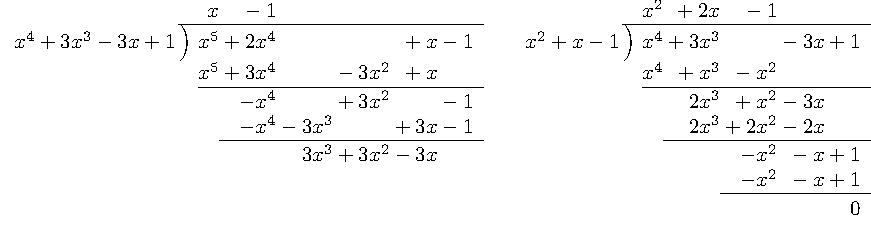
\includegraphics{emath_figures/p228_toi_i.pdf}
\end{figure}


\subsection*{p228:問-(ロ)}
\addcontentsline{toc}{subsection}{\texorpdfstring{p228:問-(ロ)}{p228:問-(ロ)}}

以下により,これらは互いに素である.

\begin{figure}[ht]
  \centering
  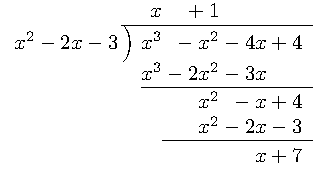
\includegraphics{emath_figures/p228_toi_ro.pdf}
\end{figure}

\newpage

\section*{p239:問1}
\addcontentsline{toc}{section}{\texorpdfstring{p239:問1}{p239:問1}}

\subsection*{p239:問1-(イ)}
\addcontentsline{toc}{subsection}{\texorpdfstring{p239:問1-(イ)}{p239:問1-(イ)}}


\begin{tleftbar}
  計算すると以下のようになる:
  \begin{align*}
    {x_1}^2 + {x_2}^2+\dots+{x_n}^2 & = \left (\sum_{i=1}^{n} x_i \right )^2 - 2\sum_{1\leqq i < j \leqq n} x_j x_k \\
                                    & = (x_1+x_2+\dots+x_n)^2 - 2(x_1 x_2 + x_1 x_3 + \dots + x_{n-1} x_n)
                                    & = s_1^2 - 2s_2.
  \end{align*}
\end{tleftbar}


\subsection*{p239:問1-(ロ)}
\addcontentsline{toc}{subsection}{\texorpdfstring{p239:問1-(ロ)}{p239:問1-(ロ)}}
\begin{tleftbar}
  計算すると以下のようになる:
  \begin{align*}
    {x_1}^3 + {x_2}^3+\dots+{x_n}^3 & = \left (\sum_{i=1}^{n} x_i \right )^3 - 3\left (\sum_{i=1}^{n} x_i \right ) \left(\sum_{1 \leqq i <j \leqq n} x_i x_j \right) + 3\sum_{1\leqq i < j < k \leqq n} x_i x_j x_k \\
                                    & = (x_1+x_2+\dots+x_n)^3 -3 (x_1+x_2+\dots+x_n)(x_1 x_2 +x_1 x_3 + \dots + x_{n-1} x_n)                                                                                        \\
                                    & \quad  +3(x_1 x_2 x_3 + x_1 x_2 x_4 + \dots + x_{n-2} x_{n-1} x_n)                                                                                                            \\
                                    & = s_1^3 -3s_1 s_2 + 3s_3.
  \end{align*}
\end{tleftbar}

\section*{p239:問2}
\addcontentsline{toc}{section}{\texorpdfstring{p239:問2}{p239:問2}}

\subsection*{p239:問2-(イ)}
\addcontentsline{toc}{subsection}{\texorpdfstring{p239:問2-(イ)}{p239:問2-(イ)}}


\kakko{補題}

\[
  (a+b+c)(a^2+b^2 +c^2 -ab - bc -ca) = a^3 + b^3 + c^3 -3abc
\]

\begin{tleftbar}
  まず,
  \[
    (x-y)+(y-z)+(z-x) =0.
  \]
  これをふまえ,補題において$a=x-y$,$b=y-z$,$c=z-x$とおくと,
  \begin{align*}
     & 0 = (x-y)^3 + (y-z)^3 + (z-x)^3 - 3(x-y)(y-z)(z-x)           \\
     & \therefore ~ (x-y)^3 + (y-z)^3 + (z-x)^3 = 3(x-y)(y-z)(z-x).
  \end{align*}
\end{tleftbar}


\subsection*{p239:問2-(ロ)}
\addcontentsline{toc}{subsection}{\texorpdfstring{p239:問2-(ロ)}{p239:問2-(ロ)}}

\kakko{補題}

$a+b+c=0$のとき,
\[
  a^2 + b^2 + c^2 = -2(ab+bc+ca).
\]

\kakko{補題}

$a+b+c=0$のとき,
\[
  a^5 + b^5 + c^5 = -5abc(a^2 + b^2 + c^2).
\]

\begin{tleftbar}
  上記の2つの補題により,
  \begin{align*}
    (x-y)^5+(y-z)^5+(z-x)^5 & = -5(x-y)(y-z)(z-x)\{ (x-y)(y-z)+(y-z)(z-x)+(z-x)(x-y)\} \\
                            & = -5(x-y)(y-z)(z-x)\{(xy+xz+yz)-(x^2+y^2+z^2)\}          \\
                            & = 5(x-y)(y-z)(z-x)\{(x+y+z)^2-3(xy+xz+yz)\}.
  \end{align*}
\end{tleftbar}

\newpage

\section*{p249:問}
\addcontentsline{toc}{section}{\texorpdfstring{p249:問}{p249:問}}


\subsection*{p249:問-(イ)}
\addcontentsline{toc}{subsection}{\texorpdfstring{p249:問-(イ)}{p249:問-(イ)}}
\begin{tleftbar}
  \begin{proof}
    体$K$の単位元について,$0=0+0$であるから,
    \begin{align*}
       & a 0=a(0+0)=a0 + a0        \\
       & \therefore ~ a0 = a0 + a0
    \end{align*}
    $K$は加法について可換群であるから,$a0$の逆元$-a0$が$K$に存在する.これを用いると,
    \begin{align*}
       & a0 + (-a0) = a0 + a0 + (-a0)    \\
       & \therefore ~ 0 = a0 + a0 +(-a0)
    \end{align*}
    ここで,
    \begin{align*}
      a0 + a0 +(-a0) & =a0+ \{a0+(-a0)\} \\
                     & = a0 + 0          \\
                     & = a0
    \end{align*}
    となるから,$0=a0$である.$0=0a$についても同様.
  \end{proof}
\end{tleftbar}

\subsection*{p249:問-(ロ)}
\addcontentsline{toc}{subsection}{\texorpdfstring{p249:問-(ロ)}{p249:問-(ロ)}}
\begin{tleftbar}
  \begin{proof}
    $a \ne 0$とする.このとき,$a$の逆元$a^{-1} \in K$が存在し,$ab=0$の両辺に$a^{-1}$をかけると,
    \begin{align*}
      a^{-1} (ab)   & = a^{-1} 0 \\
      (a^{-1}a)b    & =0         \\
      1b            & =0         \\
      \therefore~ b & =0
    \end{align*}
    である.これと$b \ne 0$を仮定したときの同様の考察により,$ab=0$のとき,$a=0$または$b=0$である.
  \end{proof}
\end{tleftbar}

\newpage

\section*{p255:1}
\addcontentsline{toc}{section}{\texorpdfstring{p255:1}{p255:1}}
\begin{tleftbar}
  \begin{proof}
    $a,b,c \in H$について,$G$の演算により,$a(bc)=(ab)c$が成り立ち,このことから結合法則は成立する.

    また,仮定より$H \ne \varnothing $なので,$x \in H$をひとつとり,$a=x$,$b=x$とすると,
    \[
      ab^{-1} = x x^{-1}=e
    \]
    となり,仮定から$e$は$H$の元である.よって$H$は単位元を持つ.

    次に,$ a=e$,$b=x$とすると,
    \[
      ab^{-1}=ex^{-1}=x^{-1}
    \]
    となり,仮定により$x^{-1}$は$H$の元である.よって$H$の任意の要素は逆元を持つ.

    上の考察により,どの要素も逆元を持つので,$a=x$,$b=y^{-1}$とすると,
    \[
      ab^{-1}=x(y^{-1})^{-1} = xy.
    \]
    これは$H$の元であるから,$H$は$G$の演算について閉じている.

    以上の考察から,
    \begin{itemize}
      \item $H$は$G$の演算について閉じている
      \item $H$の元は$G$の演算について結合法則を満たす
      \item $H$は単位元$e$を持つ
      \item $H$の任意の要素は逆元を持つ
    \end{itemize}
    ということがわかり,$H$は$G$の部分群である.
  \end{proof}
\end{tleftbar}

\begin{column}
  本題にはあまり関係のない余談ですが,群が空集合でないことは群の定義からただちに従います.
\end{column}

\newpage
\begin{thebibliography}{9}
  \bibitem{saito} 齋藤正彦『線型代数入門』,東京大学出版会,1966
\end{thebibliography}

\end{document}